\documentclass[letterpaper,12pt,oneside]{book}
%\usepackage[a4paper,includeall,bindingoffset=0cm,margin=2cm,marginparsep=0cm,marginparwidth=0cm]{geometry}
\usepackage[top=1.3in, left=1.25in, right=1.25in, bottom=1in]{geometry}
\usepackage{bachelorstitlepageUNAM}
\usepackage[toc,page]{appendix}
\usepackage[utf8]{inputenc}
\usepackage{float}
\usepackage{pdfpages}
\usepackage{subcaption}
\usepackage{graphicx}
\usepackage{subcaption}
\usepackage[hyperfootnotes=false]{hyperref}
\usepackage[T1]{fontenc}
\usepackage[utf8]{inputenc}
\usepackage[english,es-nodecimaldot,es-tabla]{babel}
\usepackage{graphicx}
\usepackage{tikz} 
\usepackage{tocloft}
\graphicspath{{./figs/}}
\usepackage{setspace}
\usepackage[super]{nth}
%\usepackage[round]{natbib}
\usepackage{amsmath}
\renewcommand\cftsecpresnum{\S}
\renewcommand\cftsubsecpresnum{\S}   


\begin{document}
%------------------------------

    \begin{titlepage}
        \thispagestyle{empty}
        \begin{minipage}[c][0.17\textheight][c]{0.25\textwidth}
            \begin{center}
                
\includegraphics[width=3.5cm, height=3.5cm]{Escudos/Escudo-UNAM.pdf}
            \end{center}
        \end{minipage}
        \begin{minipage}[c][0.195\textheight][t]{0.75\textwidth}
            \begin{center}
                \vspace{0.3cm}
                \textsc{\large Universidad Nacional Aut\'onoma de M\'exico}\\[0.5cm]
                \vspace{0.3cm}
                \hrule height2.5pt
                \vspace{.2cm}
                \hrule height1pt
                \vspace{.8cm}
                \textsc{Facultad de Ciencias}\\[0.5cm] %
            \end{center}
        \end{minipage}

        \begin{minipage}[c][0.81\textheight][t]{0.25\textwidth}
            \vspace*{5mm}
            \begin{center}
                \hskip2.0mm
                \vrule width1pt height13cm 
                \vspace{5mm}
                \hskip2pt
                \vrule width2.5pt height13cm
                \hskip2mm
                \vrule width1pt height13cm \\
                \vspace{5mm}
                
\includegraphics[height=4.0cm]{Escudos/Escudo-FCIENCIAS.pdf}
            \end{center}
        \end{minipage}
        \begin{minipage}[c][0.81\textheight][t]{0.75\textwidth}
            \begin{center}
                \vspace{1cm}

                {\large\scshape  %}\\[.2in]
\textbf{Optical tweezers implementation for a single-cell study of Diatoms:} \\[0.5em]
{\small Exploration of trapping performance and the photonic properties of frustules}
                \vspace{2cm}            
                
                \textsc{\LARGE T\hspace{1.5cm}E\hspace{1.5cm}S\hspace{1.5cm}I\hspace{1.5cm}S}\\[0.5cm]
                \textsc{\large para obtener el t\'itulo de:}\\[0.5cm]
                \textsc{\large Físico}\\[0.5cm]
                \textsc{\large que presenta:}\\[0.5cm]
                \textsc{\large {Raymundo Vázquez Martínez.}}\\[2cm]          

                \vspace{0.5cm}

                {\large\scshape Tutor:\\[0.3cm] {Remigio Cabrera Trujillo\\ 
%Dr. Sinhué A. R. Haro Corzo}}\\[.2in]

                \vspace{0.5cm}

                \large{Ciudad Universitaria, CD. MX.,}{ }{2025}
            \end{center}
        \end{minipage}
    \end{titlepage}



%---------------------------------
\frontmatter
%\maketitle

%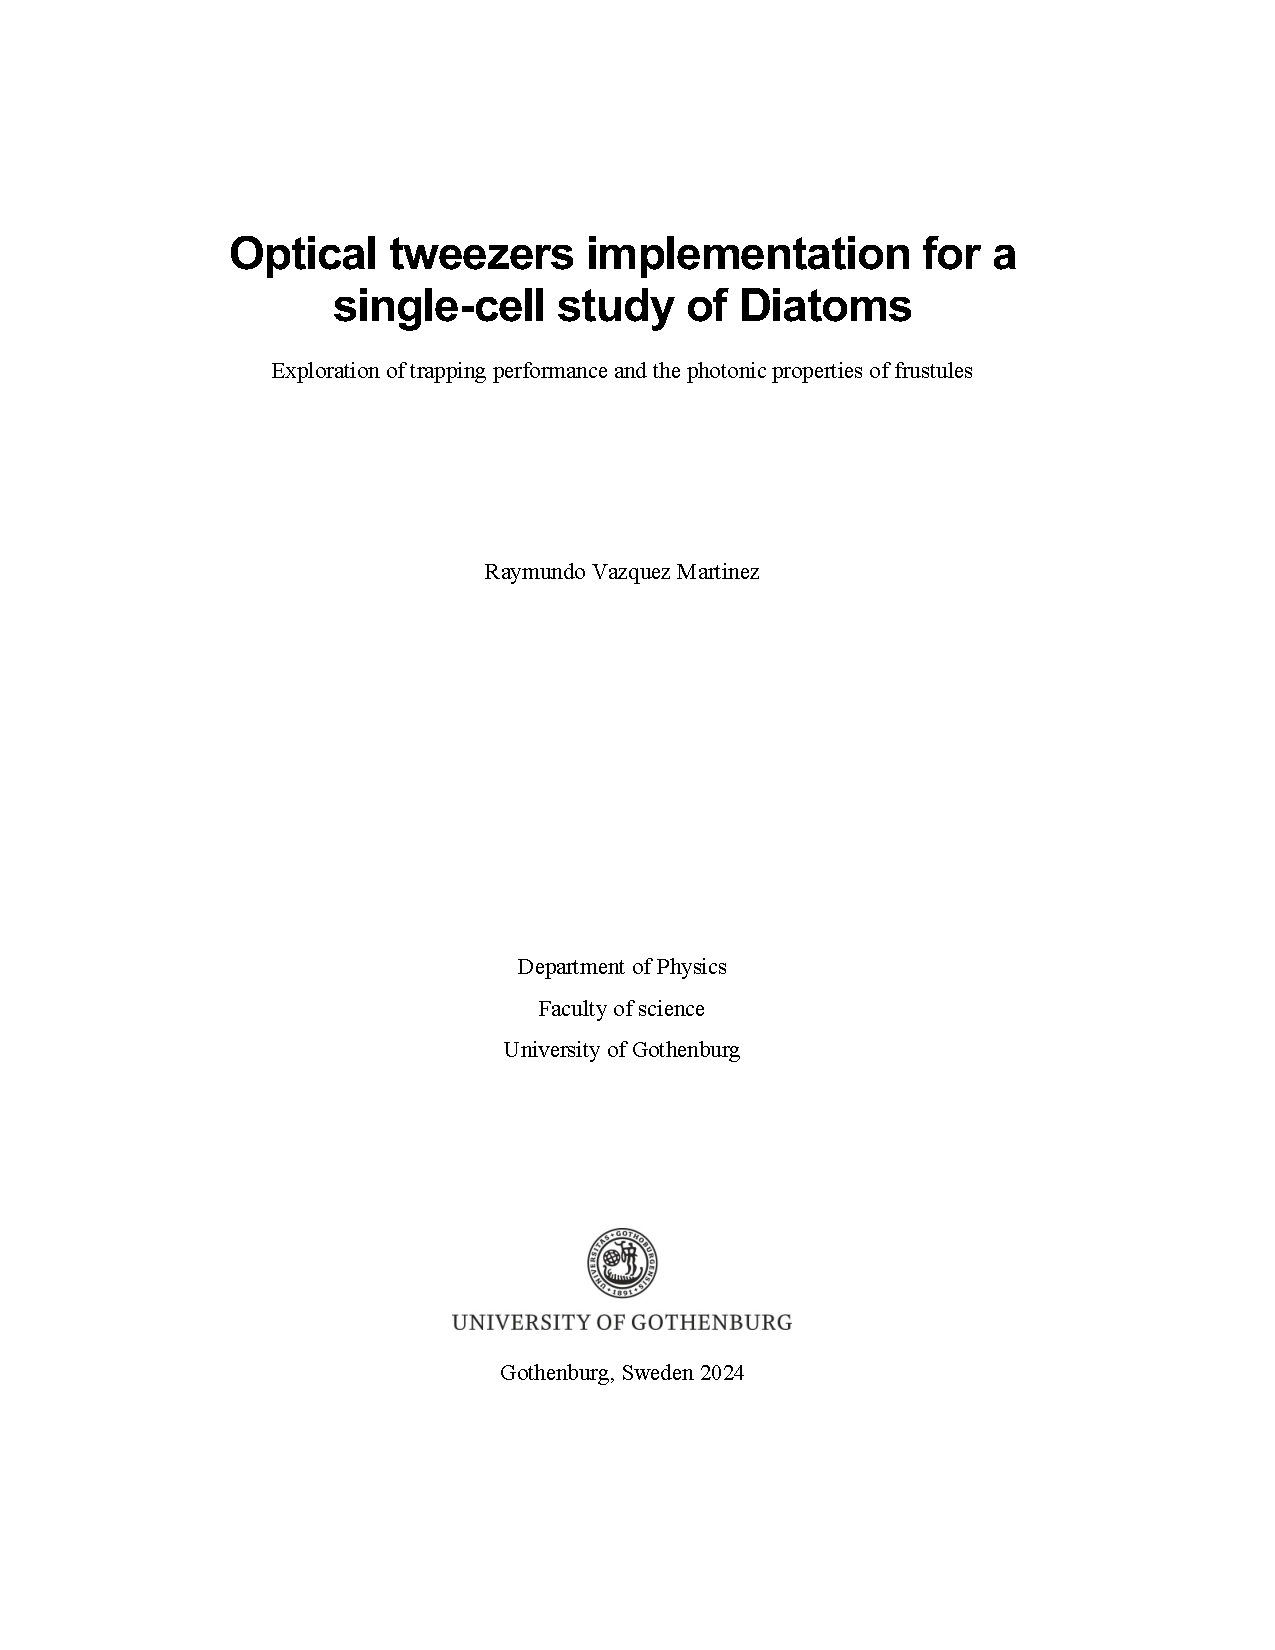
\includepdf[page={-}]{cover.pdf}
\begin{flushright}%
  \emph{Dedicatoria ...}
  \newline A mi madre. Como en las guajiras.
  \thispagestyle{empty}
\end{flushright}
\newpage
\vspace*{\fill}

% Center the text
\begin{center}
    This work was conducted in Professor Dag Hanstorp's lab at the University of Gothenburg, under the auspices of the Linnaeus-Palme Foundation.
\end{center}

% Add more vertical space to balance the page
\vspace*{\fill}
\chapter*{}
\section*{Abstract}
Diatoms are single-celled algae found in almost every area where water is present on Earth. The diatoms have the crucial property of being surrounded by a shell made of silica (frustule). The frustule is encrusted with periodic pores and ribs, endowing these single-cell organisms with optical properties that, for some species, are reminiscent of photonic crystals. Despite the diatoms' interesting photonic properties, the evolutionary reason of the frustules is not determined.\\\noindent
This work presents the implementation of optical tweezers and microfluidic devices for manipulating artificial silica bodies and diatomic algae. The optical manipulation was achieved for diatoms of different species with either spherical or bilateral symmetry and artificial silica particles of different sizes below 25 micrometers. In particular, the \textit{Nitzchia Sp.1}, \textit{Phaeodactylum tricornutum}, \textit{Navicula Sp. 12}, \textit{Marine pennate}, and \textit{Thalassiosira pseudonana} diatom species were optically manipulated. The use of optical tweezers allows for a single-cell study of these algae. As a continuation of the biological experiments of this work, and similarly to the first applications of optical tweezers to biology performed by Ashkin, this work shows the manipulation and "opticution" (dead by light) of yeast cells. Finally, the media's flow velocity to remove the particles from the optical trap was measured for different laser powers. Specifically, measurements were performed with the microfluidic system syringe pump for the \textit{Thalassiosira pseudonana} species and the $6.59 \mu m$ $SiO_2$ particles. This provides a quantifiable measure of the performance of the optical tweezers, which can be associated with the magnitude of the gradient force. Moreover, it provides first insights into the interaction of the frustules with light.\newpage 
\section*{Resumen}
Las diatomeas son algas fotosintéticas unicelulares que se encuentran en casi todas las áreas donde hay agua en la tierra. Las diatomeas tienen la propiedad distintiva de estar rodeadas por una carcaza hecha de sílice (frústula). La frústula está incrustada con poros y rejillas que aparecen de manera periódica en su arquitectura, dotando a estos organismos unicelulares de propiedades ópticas que, para algunas especies, se asemejan a los cristales fotónicos. A pesar de las interesantes propiedades fotónicas de las diatomeas, la razón evolutiva de las frústulas aún no está determinada.

\\ \noindent Este trabajo presenta la implementación de pinzas ópticas y dispositivos microfluídicos para manipular cuerpos de sílice artificiales y algas diatomeas. La manipulación óptica se logró para diatomeas de diferentes especies con simetría esférica o bilateral y partículas de sílice artificiales de diferentes tamaños por debajo de los 25 micrómetros. En particular, se manipularon ópticamente las especies de diatomeas \textit{Nitzchia Sp.1}, \textit{Phaeodactylum tricornutum}, \textit{Navicula Sp. 12}, \textit{Marine pennate}, y \textit{Thalassiosira pseudonana}. El uso de pinzas ópticas permitió el estudio de células individuales para estas algas, que usualmente se estudian en conjunto. Como continuación de los experimentos biológicos de este trabajo, y de manera similar a las primeras aplicaciones de las pinzas ópticas a la biología realizadas por Ashkin, este trabajo muestra la manipulación y la "opticución" (muerte por luz) de células de levadura. Finalmente, se midió la velocidad del medio en los canales microfluidicos para remover las partículas de la trampa óptica para diferentes potencias del láser. La medición se realizó con la bomba de jeringa del sistema microfluídico para la especie \textit{Thalassiosira pseudonana} y las partículas $SiO_2$ de $6.59 \mu m$. Esta medición proporciona una medida cuantificable del rendimiento de las pinzas ópticas, que puede asociarse con la magnitud de la fuerza de gradiente. Además, proporciona primeros indicios sobre la interacción de las frústulas con la luz.
%Se estudia la implementación de pinzas ópticas para la manipulación de cuerpos de sílice y entidades biológicas específicas. Dentro del conjunto de cuerpos de sílice atrapados en este trabajo, encontramos partículas de sílice esféricas artificiales y, más especialmente, algas diatomeas (Diatoms). La manipulación con las pinzas ópticas se obtuvo para diatomeas de diferentes especies con simetría distintiva (simetría esférica o bilateral) y partículas de sílice artificiales de diferentes tamaños. Las diatomeas tienen la propiedad crucial de estar rodeadas por una coraza hecha de sílice (frustule). Estas cáscaras tenien intrrincados poros en su superficie. Dando continuidad a los experimentos biológicos de este trabajo, y de manera similar a las primeras aplicaciones de pinzas ópticas en biología realizadas por Ashkin, se muestra la manipulación y "opticutión" (muerte por luz) de células de levadura. Finalmente, se explora la manipulación de las partículas de sílice artificiales y especies de diatomeas mientras fluyen a través de canales microfluídicos, encontrando diferencias entre la estabilidad de las pinzas ópticas al atrapar las diatomeas céntricas hechas de sílice (Thalassiosira pseudonana) y las partículas esféricas de sílice artificiales.
\chapter{Acknowledgments}
\spacing{1.5}%\doublespacing
First, I wish to express my heartfelt gratitude to all those who have contributed, in some way, to the successful completion of this work. Therefore, I would like to thank:
\begin{itemize}
  \item Professor Dag Hanstorp for welcoming me at the University of Gothenburg, and for providing invaluable support, help, and guidance throughout this work. 
  \item Jonas Enger, and Yogeshwar Nath Mishra for supervising my work in the lab, and the help provided to the completion of this work. 
  \item Javier Tello Marmolejo for the introduction to the lab, and share of his knowledge in the field of optical trapping, besides teaching me good lab practices and enhancing my learning curve. 
  \item Oscar Isaksson for making Mondays more enjoyable, and for being there in my progress and drawbacks in the lab.
  \item Angela Wulff for the invaluable lectures on Diatoms, and for providing the samples for this work.
  \item Martin Selin for providing me with his silica particles, and the discussions we had regarding the performance of the optical tweezers.
 \item Charlotte Blomqvist for providing the microfluidic system of this work, and the introduction to the PDMS lab. 
  \item Dr. Ricardo Méndez Fragoso for the help in installing the laser device, and the company during the research group trips.
  \item Dr. Remigio Cabrera Trujillo for being the connection between the University of Gothenburg and the National Autonomous University of Mexico, which allowed for my stay in Gothenburg in the first place. 
  \item Ludi, Mats, and Richard for all the technical help, and tools provided for this work.
  \item Hinduja, Megha, Rachel,
Keerthana, Veena, and Meera, for the moments we shared in the lab, and the office that made my stay in Gothenburg more remarkable. 
\item Constanza, Yaz, Andrea, and Valeria, for being my close friends from Mexico. Especially Coni, for all the time we spend together in the lab.
\item All the PhD and Master's students from Chalmers, and Gothenburg University I met while wandering through the corridors. 
\item The Linnaeus-Palme Foundation for making all this possible.
\item My family in Mexico for staying close.
\item My friends from UNAM, and Gothenburg.
\item Juana Cristina for being with me along the way, and for all the happiness during the tough moments.
\item My sister for being interested in my deeds, and being one of my biggest motivations.
\item My mom, for all the things beyond words to express. 

\end{itemize}

%\chapter{Notation}


\tableofcontents
%\listoffigures

    
\mainmatter

\chapter{Introduction} 
The idea that light can exert forces on an object is old. Johannes Kepler, in the \nth{17} century, had already proposed that sunlight determines the orientation of comet tails \cite{kepler}. Back then, only in astronomy, where light intensities are immense and distances are long, did we see an important effect of the radiation pressure \cite{ashkin1997optical}. The development of electromagnetic theory brought a mathematical framework to investigate the effect of radiation pressure on objects \cite{maxwell1865viii}, and this led to the first successful experimental investigations by Nichols, Hull, and Lebedev on the detection of radiation pressure \cite{nichols1901preliminary,lebedev1883experimental}.  The topic was mainly forgotten due to the extreme minuteness of the effects of radiation pressure in terrestrial affairs \cite{ashkinhistory}.
However, with the advent of the laser, we could use high intensities and high-intensity gradients of continuous wave coherent light beams to take advantage of the radiation pressure for applications at smaller scales \cite{ashkin1997optical,townes2002laser}. \\ 
\indent Arthur Ashkin and Joseph Dziedzic, through a series of experiments starting in 1969, reported that a tightly focused laser beam could manipulate and hold small particles (optical tweezing) \cite{ashkin1970acceleration,ashkin1970atomicdeflection,ashkin1986observation}.
  Over the years to come, optical manipulation would be established as a powerful and versatile tool in research fields where small particles play a significant role. In the field of atomic physics, Steven Chu, Claude Cohen-Tannoudji and William D. Phillips were awarded the Physics Nobel Prize in 1997 “for development of methods to cool and trap atoms with laser light” \cite{NobelPrizeChu}. Optical tweezers enabled the manipulation and trapping of manufactured nanostructures such as quantum dots, carbon nanotubes, and two-dimensional crystals, offering new advances for the assembly of individual and multiple nanoparticles with force measurement on the femtonewton scale \cite{marago2013optical}.
%\cite{weitenberg2011quantum,mazzanti2023trapped},
Since the early 1990's optical tweezers have become widely used to assist biology research \cite{jones2015optical}, ranging from manipulation and photodamage studies of bacteria, viruses, and single cells to DNA elasticity and molecular motors studies \cite{ashkinmanipulationvirus,sowa2005directmotor,smith1996overstretchingdna}. Furthermore, “for the optical tweezers and their application to biological systems”
Arthur Ashkin was awarded the Physics Nobel Prize in 2018 \cite{NobelPrizeAsh}.\\ \indent
Another powerful tool for researching particle systems at the micrometre scale are microfluidic devices. A microfluidic device contains small channels with dimensions on the micrometre scale that are used to control and manipulate small volumes of fluids. These channels are generally made of transparent materials such as glass, silicon or polydimethylsiloxane (PDMS) \cite{nielsen2019microfluidics}, and offer several advantages over preceding methods for the study of small fluidic systems, including  high sensitivity, low sample consumption, and the extensibility of the physical and chemical properties which they can be designed with %designing for different chemical and physical properties 
 \cite{chin2012commercialization}. These advantages placed microfluidic devices as useful tools for a wide range of applications in many fields of science and engineering. In ecology, microfluidic devices provide a portable and accurate method for detecting and analyzing pollutants and contaminants in environmental samples \cite{marle2005microfluidicenviromental}. In biology, the applications include cellular studies: cell migration, proliferation, and single cell analysis in different media; or DNA molecule sequencing \cite{paegel2003microfluidicDNA}. In addition, the combination of optical tweezers and microfluidic channels has enabled further analysis of cell mechanics, interactions, and responses to stimuli, by manipulating individual cells and particles in the channels \cite{wang2011enhancedmicroandopti}. Mihrimah Ozkan \textit{et al.} reviewed the usage of optical manipulation of particles and biological cells in microfluidic devices \cite{ozkan2003opticalandmicrofluidicsreview}. 
%Microfluidic channels are small channels with dimensions on the micrometer scale that are used to control and manipulate small volumes of fluids. These channels are typically made of materials such as glass, silicon, or polymers and are often used in microfluidic devices, which are used for a variety of applications in fields such as chemistry, biology, and engineering.
\\\indent Diatoms are single-celled photosynthetic algae \cite{round1990diatoms}, occurring in
almost every area or habitat on Earth where water is present, ranging from freshwater
lakes and oceans \cite{diatomworld} to moist soils and even Antarctic ice cores \cite{iceladregional}. They are characterized by the frustule, a silica shell confining the inner cell,  synthesized from monosilicic acid during the algal growth 
 \cite{aguirre2018diatomDNAViolet}. The frustule surface is covered by regular patterns of micro- and nano-perforations (pores), which allow substance exchanges and filtering between the organism and the environment \cite{de2021underwater}. The evolutionary causes for the frustules are
not yet understood. Some authors suggest that they originated to protect the diatom DNA from UV radiation \cite{aguirre2018diatomDNAViolet}, while others suggest that mechanical protection is the main purpose \cite{hamm2003architecture}.\\\indent
Diatoms possess a good capacity for light harvesting and exploitation, proven by their contribution of around 20-25$\%$ to the global production of oxygen \cite{carbonexport}. Recent studies show that the 10–100 nm patterns of holes, slits, and ribs on the frustules are
reminiscent of the geometries of photonic bandgap structures \cite{fuhrmann2004diatoms}. In 2019, the application of light-matter interaction properties of the diatom frustules was studied by T.M.W.J Bandara \textit{et al.} showing enhance in solar cells efficiency \cite{solardiatom}. Other experimental and computational studies have shown that incorporating diatoms on the surface of light-absorbing materials enhance their efficiency \cite{chen2015numerical}. These studies involve using layers of diatoms that are placed on a sample surface. The layers are often prepared by collecting diatoms from natural environments, cleaning them, and depositing them onto a suitable substrate. In contrast, a complete single-cell characterization of the light-frustule interaction with coherent light sources remains to be investigated. These studies could shed light on the optical and biological properties of the Diatoms. 
Due to the previously mentioned applications, evaluating the frustules' optical properties is essential since they could supply a greener and low-cost alternative to artificial nanostructures with these capabilities.  \\\indent 
In this work, I proposed to investigate the behavior of different species of diatoms when exposed to different wavelengths and surroundings using optical tweezers for controlled manipulation and quantifiable force detection. With these experiments, I aim to identify wavelength-specific variations in light tolerance and photonic properties across different species of diatoms. The long-term goal is to provide an exhaustive study of diatom species with optical tweezers,  including measuring external forces, changing media and light sources' effects on its reproduction processes,  and characterizing the photonic properties of the frustules for different wavelengths. This study will add to the previous works done with multi-cell arranges, with a confined single-cell study. %Characterize the properties of light-matter interactions between different symmetries and species of diatoms, morever  compare with man-made structures.   
%In particular, in this project, I studied the behaviour of diatoms frustules for different species using optical tweezers. The first experiments show the capability of optical tweezers to contactless manipulate $SiO_2$ industrial particles of different sizes on the micrometre scale. Transitioning to the biological part, I showed yeast cells' manipulation and opticution (death by light), and trapping of different diatom species. Assisted with microfluidic devices, I compared the behaviour of spheric diatoms and man-made Silica particles. %I could write that the first studies were made by ashkin in manipulating silica partiles, and the studies of microfluidic channels to study diatoms for the first time. Historical part.  
\chapter{Theoretical Background.}
This chapter presents the theoretical concepts necessary to understand the tools, methods and subjects of study employed in this work.
\section{Diatoms}
%Diatoms are single-celled photosynthetic algae comprising a diverse group of organisms characterized by their unique cell walls of silica ($SiO_2$). These cell walls are constructed during algal growth, and provide them with a distinctive glass-like appearance and are at the foundation of their taxonomy. 
%There exist over 100,000 diatom species, categorized based on the configuration of their glass enclosures. Traditionally we can dived them into two broad categories based on the symmetry of the frustule; the centrict and the pennate diatoms.

Diatoms are single-celled algae comprising a diverse group of organisms characterized by their unique cell walls of silica ($SiO_2$). These cell walls, called frustules, are formed during the algal growth and provide them with their distinctive glass-like appearance \cite{aguirre2018diatomDNAViolet}. The frustules also play a fundamental role in diatom taxonomy and classification. There are over 100,000 species of diatoms identified from almost every body of water ranging from freshwater lakes and oceans
to moist soils and even Antarctic ice cores \cite{iceladregional,aguirre2018diatomDNAViolet}. The categorization comes from the configuration of their silica enclosures. Traditionally, diatoms can be broadly classified based on their frustule symmetry into two main categories: centric and pennate diatoms \cite{diatomworld}. Centric diatoms exhibit radial symmetry, with their frustules forming circular shapes. Examples of centric diatoms include \textit{Cyclotella}, \textit{Stephanodiscus}, and \textit{Thalassiosira} (see figure \ref{centric diatoms}). 
On the other hand, pennate diatoms display bilateral symmetry, with elongated frustules that resemble boats or surf boards. %They consist of two valves, an epivalve (larger) and a hypovalve (smaller). 
\textit{Navicula}, \textit{Pinnularia}, and \textit{Fragilaria} are common examples of pennate diatoms (see figure \ref{pennate diatoms}).
%Centric diatoms.
\begin{figure}[H]
     \centering
     \begin{subfigure}[b]{0.3\textwidth}
         \centering
         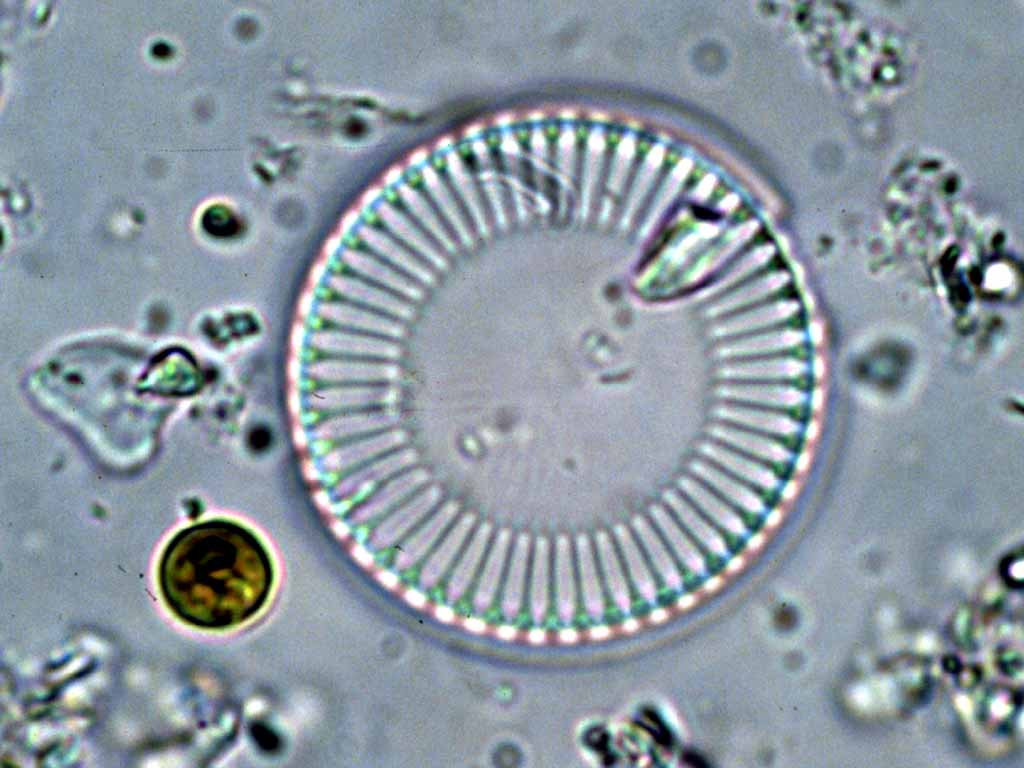
\includegraphics[width=\textwidth, height=4.5cm]{Imagesalgeacentric/Cyclotellameneghiniana.jpeg}
         \caption{  }
         \label{fig:y equals x}
     \end{subfigure}
     \hfill
     \begin{subfigure}[b]{0.3\textwidth}
         \centering
         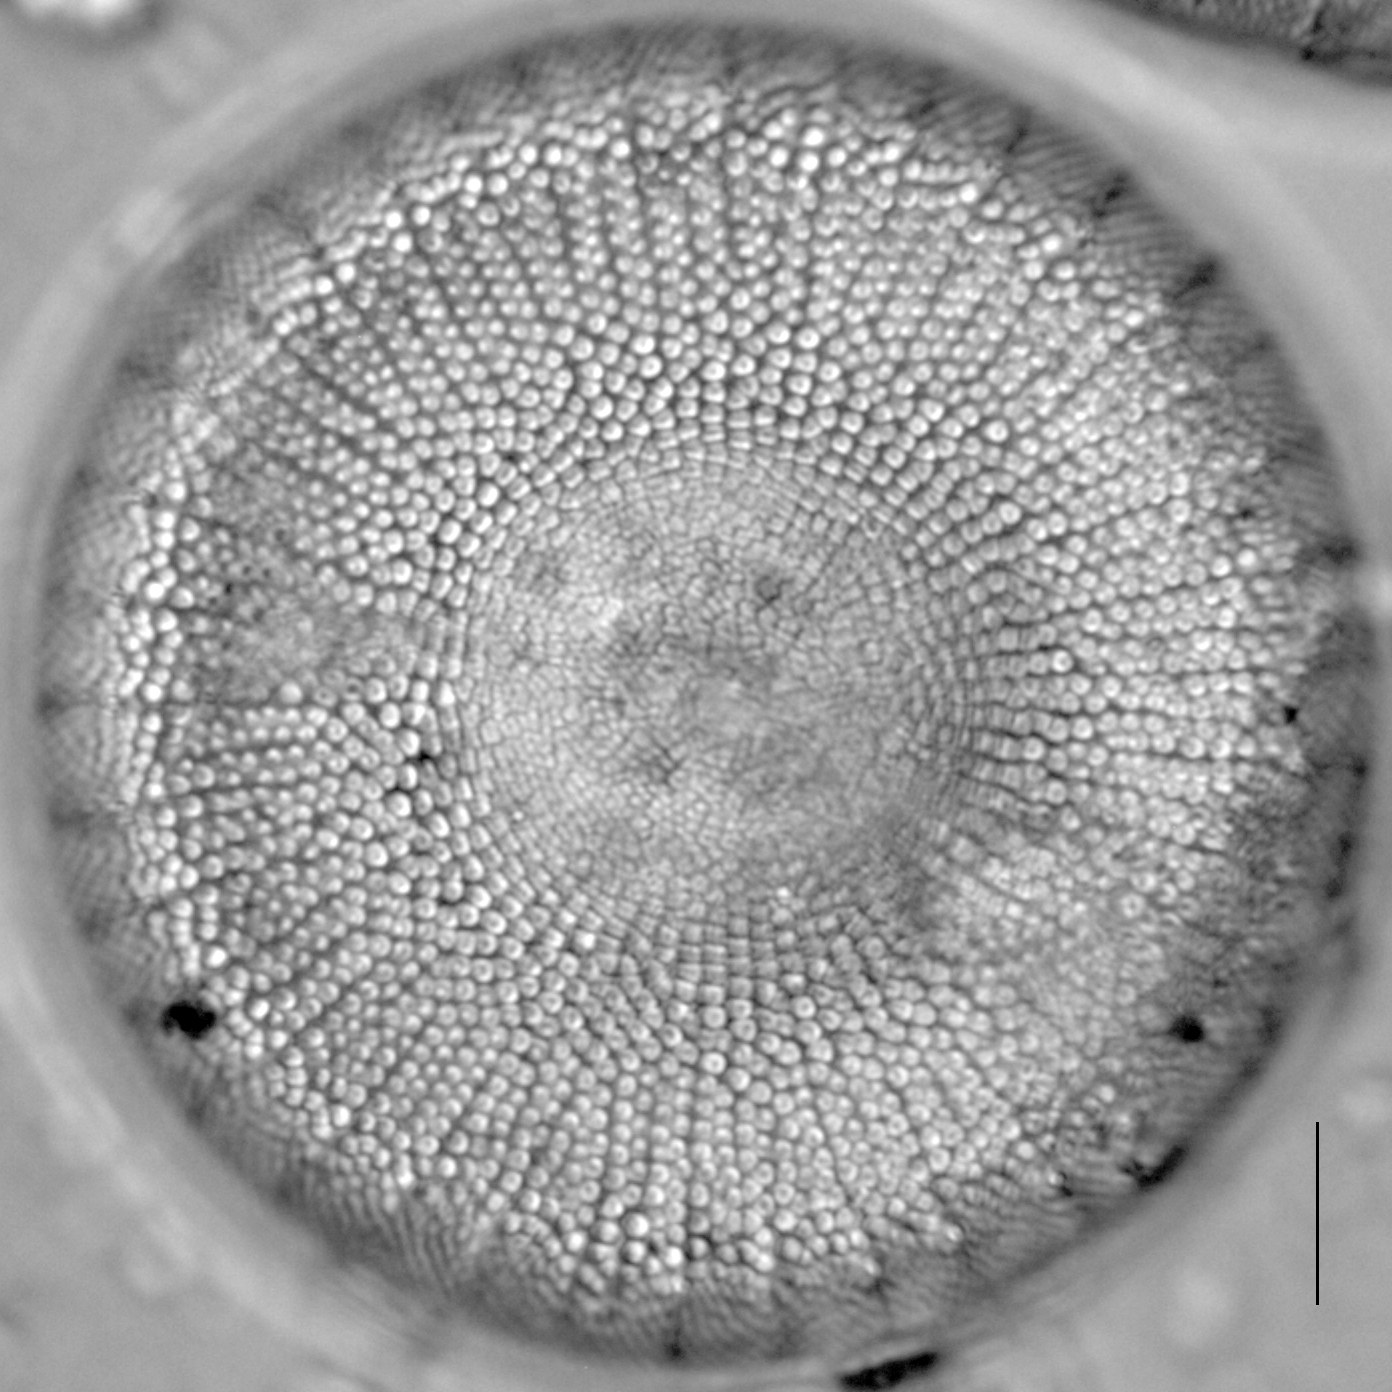
\includegraphics[width=\textwidth, height=4.5cm]{Imagesalgeacentric/Stephanodiscus_L-4-58_6_1.jpeg}
         \caption{}
         \label{fig:three sin x}
     \end{subfigure}
     \hfill
     \begin{subfigure}[b]{0.3\textwidth}
         \centering
         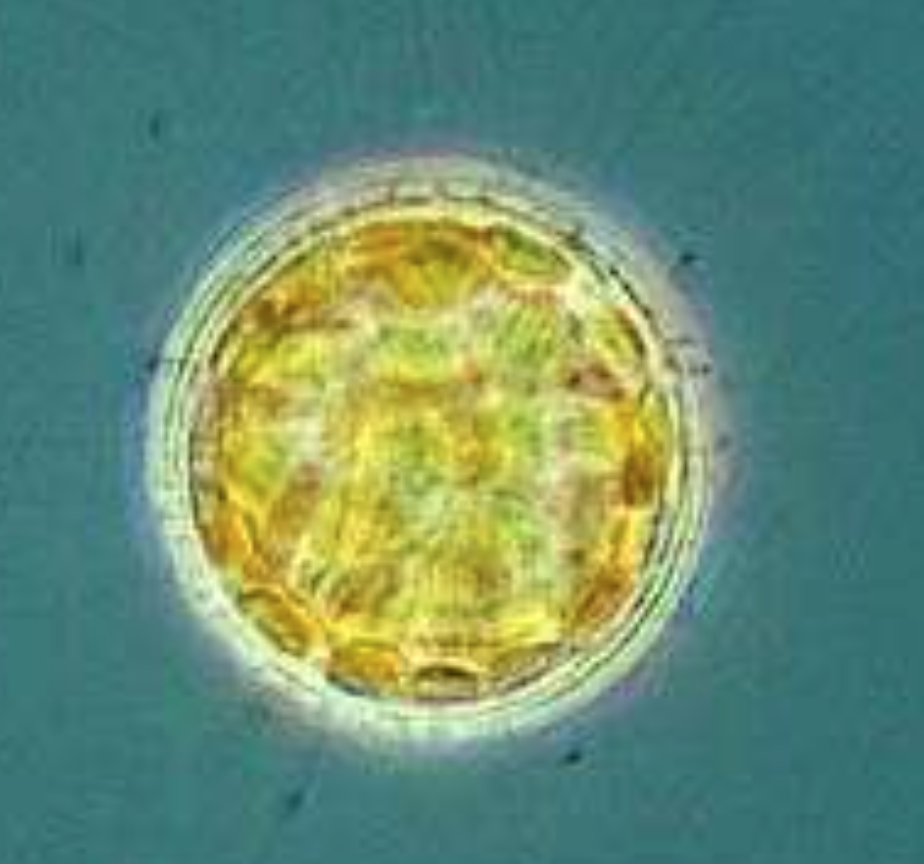
\includegraphics[width=\textwidth, height=4.5cm]{Imagesalgeacentric/Screen Shot 2023-06-18 at 8.33.22 PM.png}
         \caption{}
         \label{fig:five over x}
     \end{subfigure}
        \caption{Examples of centric diatoms. 
(a) \textit{Cyclotella meneghiniana}, image taken from \cite{cyclotella}. (b) \textit{Stephanodiscus reimeri}, image taken from \cite{DiatomsofNorthAmerica} (c) \textit{Thalassiosira eccentrica}, image taken from \cite{Thalassiosiraimage}.}
        \label{centric diatoms}
\end{figure}
%Pennate diatoms figure for examples. 
\begin{figure}[H]
     \centering
     \begin{subfigure}[b]{0.3\textwidth}
         \centering
         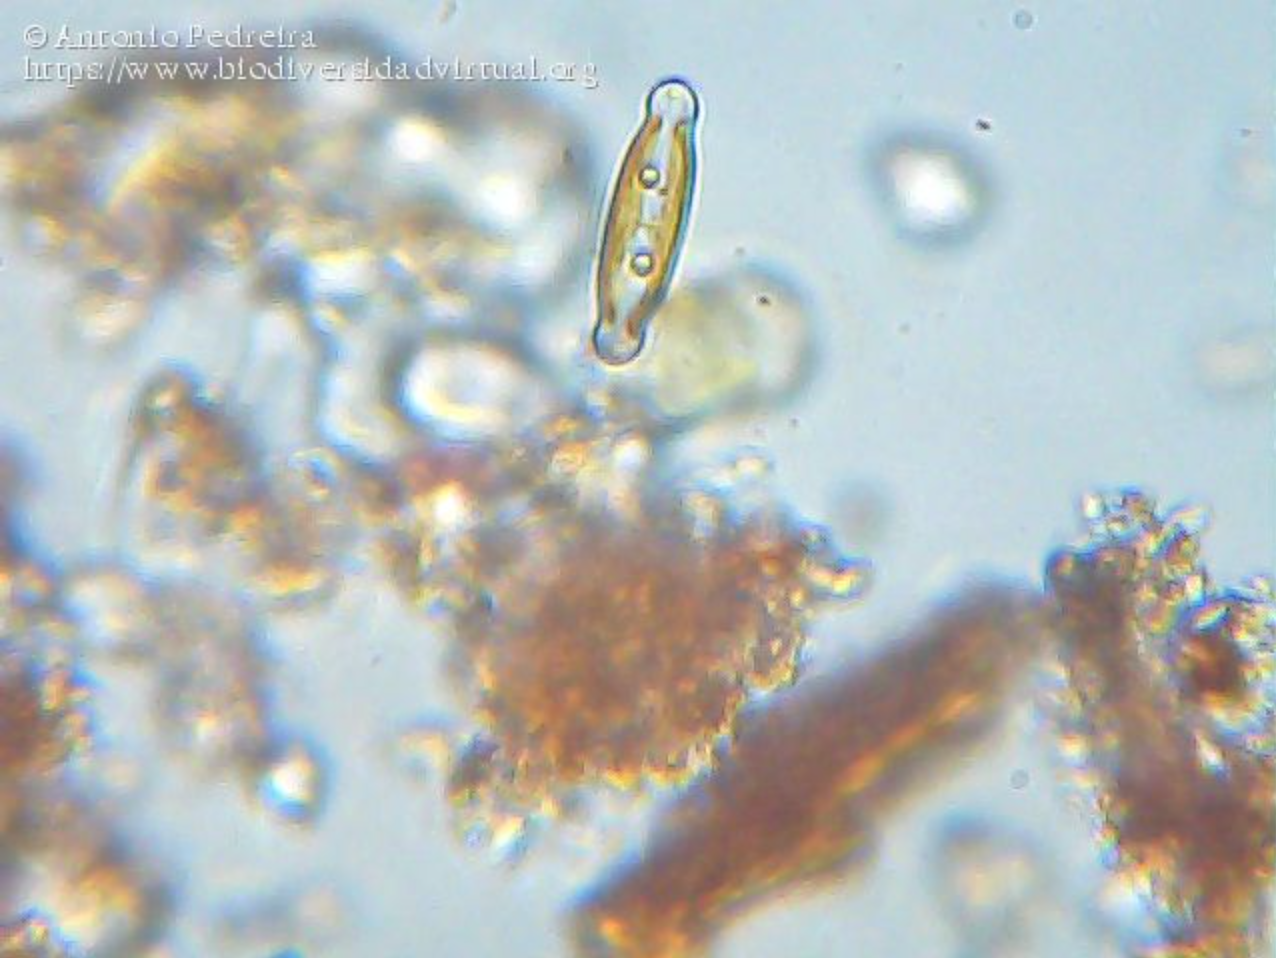
\includegraphics[width=\textwidth, height=4.5cm]{Pennate/Screen Shot 2023-06-18 at 10.14.52 PM.png}
         \caption{  }
         \label{fig:y equals x}
     \end{subfigure}
     \hfill
     \begin{subfigure}[b]{0.3\textwidth}
         \centering
         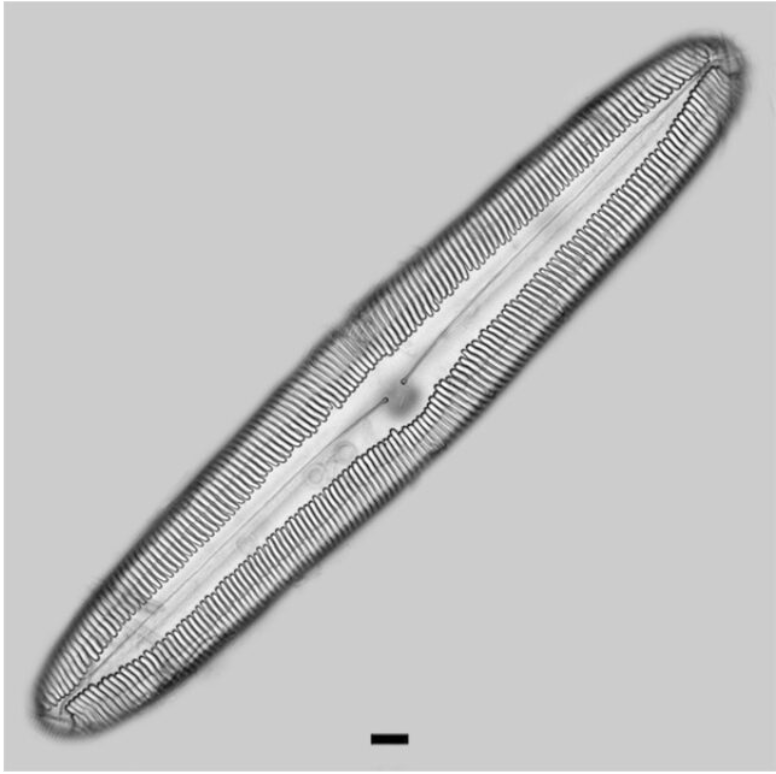
\includegraphics[width=\textwidth, height=4.5cm]{Pennate/Screen Shot 2023-06-18 at 10.25.11 PM.png}
         \caption{}
         \label{fig:three sin x}
     \end{subfigure}
     \hfill
     \begin{subfigure}[b]{0.3\textwidth}
         \centering
         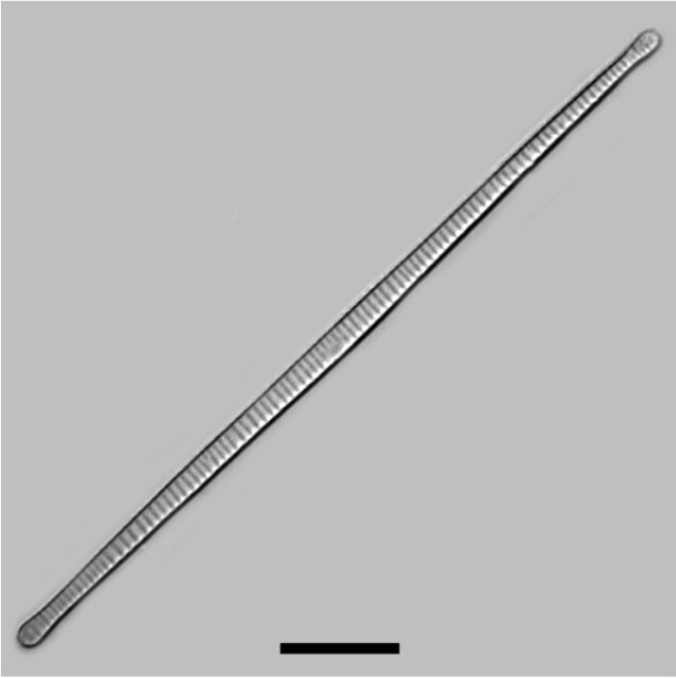
\includegraphics[width=\textwidth, height=4.5cm]{Pennate/grotestcapennate.png}
         \caption{}
         \label{fig:five over x}
     \end{subfigure}
        \caption{Examples of Pennate diatoms. 
(a) \textit{Navicula pupula}, image taken from \cite{Pedreira_2012} with permission of its author. (b) \textit{Pinnularia dariana}, image taken from \cite{DiatomsofNorthAmericadariana}. (c) \textit{Fragilaria synegrotesca}, image taken from \cite{DiatomsofNorthAmericafragilaria}.}
        \label{pennate diatoms}
\end{figure} \noindent
Over the past 100 million years, these silica structures have been amassing, resulting in the widespread accumulation of microstructured silicon oxide known as diatomaceous earth \cite{aguirre2018diatomDNAViolet}. The abundance and productivity of Diatoms make them an essential part of the aquatic food web. 
\\\noindent 
One striking aspect of the frustules is their intricate architecture with holes, slits and ribs on their surface (see figure \ref{poresfrustrules}). The frustule provides mechanical protection and filtering of substances to the cell, and in many instances, the orifices are spaced at such a distance as to prevent DNA UV damage and modify coherent laser light \cite{aguirre2018diatomDNAViolet,de2007lensless}. I showcased in the introduction that the optical properties of the frustules started many studies and could be the evolutionary cause for them.

\begin{figure}[H] 
  \begin{subfigure}[b]{0.5\linewidth}
    \centering
    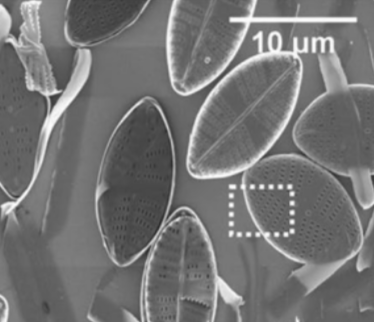
\includegraphics[width=0.75\linewidth]{Frustrulespictures/Screen Shot 2023-07-02 at 8.24.59 PM.png} 
    \subcaption[]{}
    \label{fig7:a} 
    \vspace{4ex}
  \end{subfigure}%% 
  \begin{subfigure}[b]{0.5\linewidth}
    \centering
    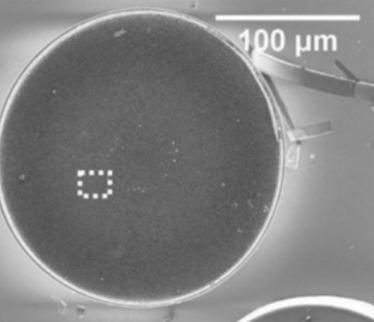
\includegraphics[width=0.75\linewidth]{Frustrulespictures/Screen Shot 2023-07-02 at 8.25.32 PM.png} 
    \subcaption[]{}
    \label{fig7:b} 
    \vspace{4ex}
  \end{subfigure} 
  \begin{subfigure}[b]{0.5\linewidth}
    \centering
    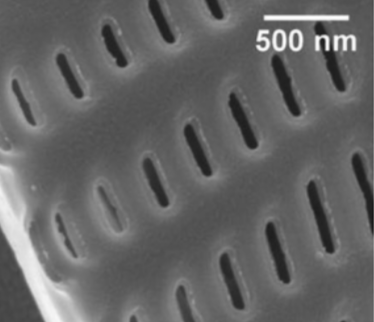
\includegraphics[width=0.75\linewidth]{Frustrulespictures/Screen Shot 2023-07-02 at 8.25.17 PM.png} 
    \subcaption[]{}
    \label{fig7:c} 
  \end{subfigure}%%
  \begin{subfigure}[b]{0.5\linewidth}
    \centering
    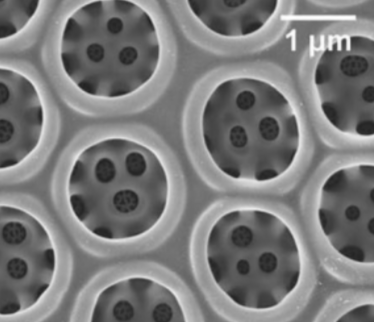
\includegraphics[width=0.75\linewidth]{Frustrulespictures/Screen Shot 2023-07-02 at 8.25.43 PM.png} 
    \subcaption[]{}
    \label{fig7:d} 
  \end{subfigure} 
  \caption{Scanning electron microscope (SEM) images of (a,c) - \emph{Navicula perminuta}, (b,d) \emph{Coscinodiscus wailesii}. Dashed rectangles in (a–b) correspond to the
magnified areas in (c–d) exhibiting the holes, slits, and ribs of the frustule's architecture. Images taken from \cite{aguirre2018diatomDNAViolet}.}
  \label{poresfrustrules} 
\end{figure}

\\In these studies, a microscope device is useful to image the diatom sample. In particular, this study of the optical properties of diatoms will use an inverted microscope to image the samples for reasons that will become evident later.


\newline\newline 
%The frustrule provides
%One striking characteristic of diatoms lies in their interaction with solar light, as evidenced by their photosynthesis process, which contributes approximately $20\%$ of the Earth's global oxygen production. 
%One striking aspect of Diatoms is their interaction with solar light.  This is proven by the fact that through photosynthesis diatoms produce about $20\%$ of the global oxygen supply. 
%As these cell enclosures is that their surfaces are neither smooth nor continuos. 
%These microscopic organisms are photosynthetic, meaning they are capable of converting sunlight into chemical energy through the process of photosynthesis. They play a crucial role in the Earth's ecosystems as primary producers, responsible for a significant portion of the world's oxygen production. In fact, it is estimated that diatoms contribute to about 20-25% of the global oxygen supply.

%Diatoms are an essential part of the food web as they form the base of many aquatic food chains. 
%They are consumed by various organisms, including zooplankton, small invertebrates, and even some fish species. Their abundance and productivity make them an important food source for higher trophic levels.
\section{Inverted Microscope}
Given the sample(specimen) placed at the stage in an inverted microscope (see figure \ref{FluorescenceM}), the imaging process starts at the lamphouse. Traditionally, the lamphouse contains a tungsten lamp, which is the primary light source. Immediately next to the lamphouse, there is a filter tray. Depending on the specific application, it will place filters to select different wavelengths or bandwidths to bathe the sample. 
\begin{figure}[H]
    \centering
    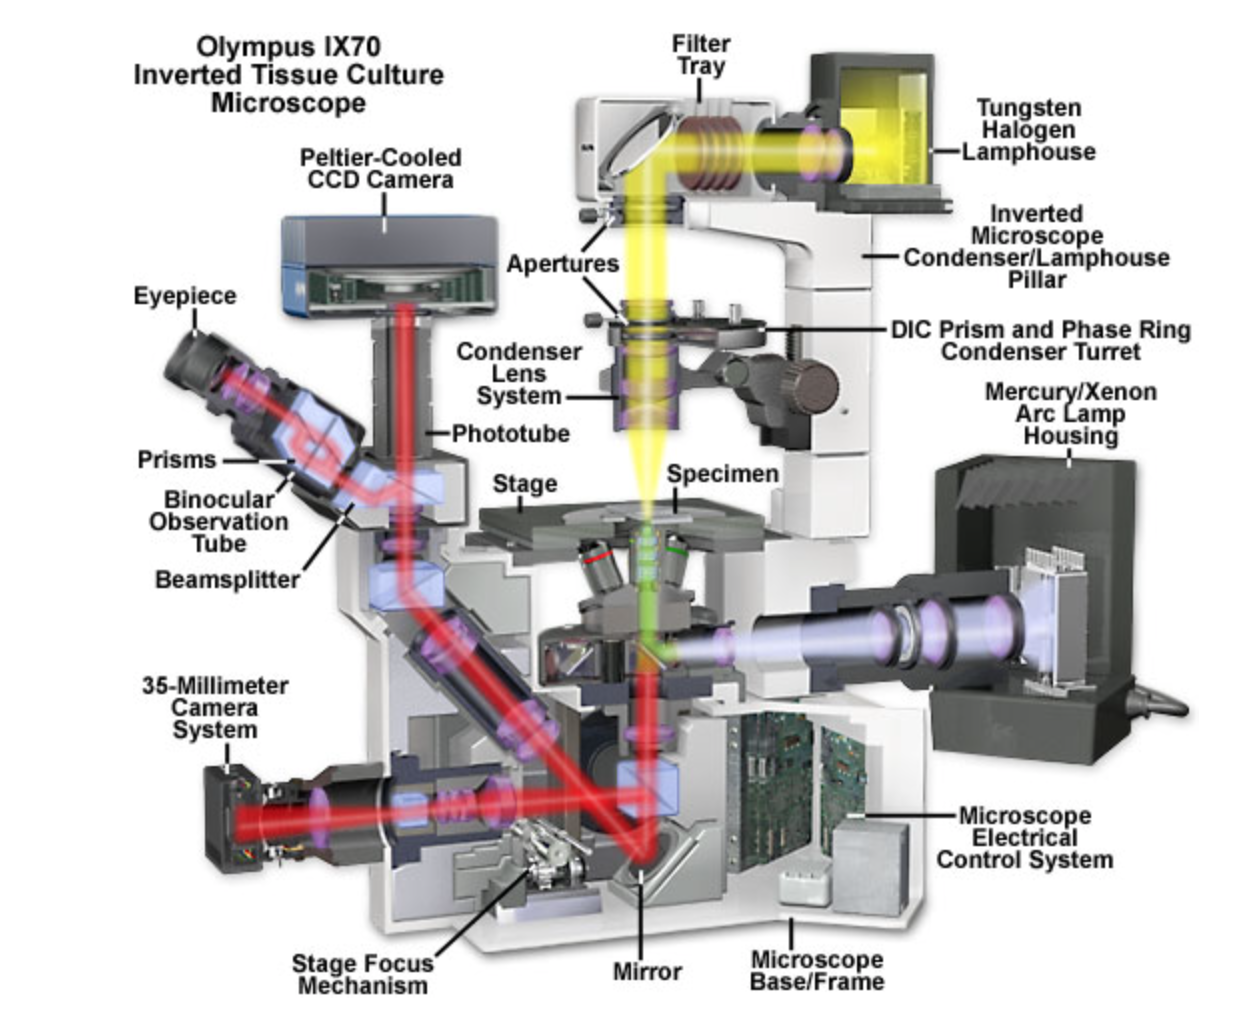
\includegraphics[scale=0.55]{Microscopeinvertedtrain.png}
    \caption{Components of an inverted microscope (Olympus IX70 microscope). Unlike a standard microscope, the inverted microscope has an illumination system and its condenser lenses above the stage. Moving the microscope objective changes the plane of focus captured by the camera. Image taken from \cite{Fester_Davidson_Abramowitz}. \label{FluorescenceM}}
    \label{Microscope inverted}
\end{figure}
\noindent The imaging process continues with the incoming light beam being shaped and cut out by an integrated aperture system positioned above the sample stand. This system selects a portion of the light that will pass through the condenser lens system. The condenser lens system can be adjusted and tuned to converge, collimate or diverge the light bathing the sample. Underneath the condenser lens system, we reach the stage, often movable in the xy plane, where we place the specimen sample. \\The most important part of the microscope comes into play at this point: the objective. The objective is a lens system that images the sample and is the closest component to the sample. It is found underneath the stage, traditionally placed in a rotatory stage, along with other microscope objectives. This rotatory stage changes the microscope objective imaging the sample. The microscope objective is selected depending on the requirements of the application. There are many aspects to consider when selecting the right one, such as magnification, numerical aperture ($NA$), working distance, and, in the case of an immersion microscope, the immersive media. The magnification refers to the scaled-up image size of the original sample, whereas the numerical aperture refers to the maximum acceptance angle for an optical system. It is defined as $NA = n \sin{\theta}$, where $\theta$ is the half-angle of the maximum cone of light that can enter or exit the optical system, and $n$ is the refractive index of the immersive media \cite{svelto2010principles}. The working distance of a microscope objective refers to the distance between the front lens of the objective and the surface of the specimen when the specimen is in focus. On the other hand, the immersive media is the substance placed on the top lens of the microscope objective to fill the gap between the microscope slide containing the sample and the objective (see figure \ref{MOWater}). 
\begin{figure}[H]
    \centering
    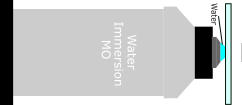
\includegraphics[angle=90]{Imagenes teoria/nikon-objective.png}
    \caption{Water immersion microscope objective (MO). The immersion media augments the amount of deviated light from the specimen captured by the microscope.}
    \label{MOWater}
\end{figure}
The light coming from the condenser lens will be scattered by the sample and collected by the microscope objective, producing an image. This imaging process is exemplified in figure \ref{imagingprocess}
\begin{figure}[H]
    \centering
    \subfloat[\centering ]{{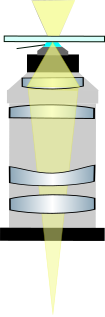
\includegraphics[scale=0.6]{rectray298722-0.png} }} \qquad
    \subfloat[\centering]{{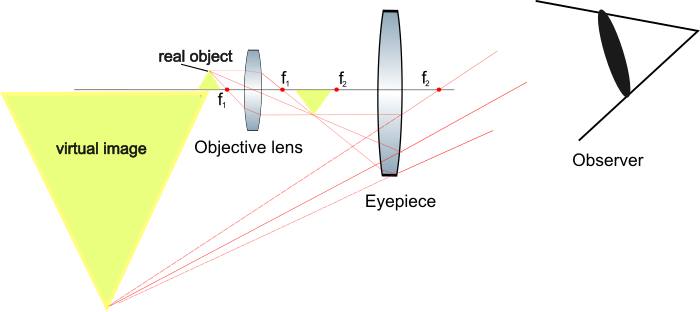
\includegraphics[scale=0.5]{g1205623227122.png} }}%
    \caption{Imaging process with the MO. (a) Refracted light by the sample passing through the lens system, composing the microscope objective. (b) The simplest model of a microscope is composed of two positive lenses: the objective and the eyepiece (focal length $f_1$ and $f_2$, respectively). The objective lens will produce a real image to the left of the eyepiece, and the latter then produces a virtual image to be captured by the observer. }
    \label{imagingprocess}%
\end{figure}
In figure \ref{imagingprocess}, we can see the refracted illumination from the sample captured by the microscope. As the size of the object we want to observe decreases, its diffraction pattern becomes larger. This occurs because smaller features cause light to diffract at wider angles, spreading the pattern over a broader area. The diffraction pattern, which encodes the structural details of the object, is then captured by the microscope's objective lens. The lens reconstructs the diffraction pattern into an image of the object through a process of interference or, in the framework of Fourier optics, by effecting an inverse Fourier transformation. \\
The ability of the microscope objective to capture as much diffracted light as possible determines its resolving power. This is quantified by the numerical aperture (NA) of the lens. A higher NA allows the objective to collect more diffracted light, enabling it to resolve finer details in the object. Ultimately, the resolution of the microscope—the level of detail we can distinguish—is limited by the wavelength of light and the NA of the objective, as described by the Abbe formula \cite{lin1986lost}.
\begin{equation}
    D=\frac{\lambda}{2 NA} \; .
\end{equation}
Where $D$ stands for resolving power (resolution), $\lambda$ is the incoming light wavelength, and $NA$ is the numerical aperture of the microscope objective. 
\\\\ %agregar it continues its path towards the final stages of the microscopes 
Underneath the microscope objectives, there is often a cage designed to place filters, beam splitters, or dichroic mirrors to filter light based on either the wavelength or polarization. The final image will be produced by the light reaching the mirror shown in figure \ref{Microscope inverted}. Then it can be seen at the different exits of the microscope with the eyepiece or the camera that can be placed at these outlets of the microscope.


%In an inverted microscope the light source bathing the sample and condenser lens are on the top, above the stage with the sample (see figure \ref{Microscope inverted}).
%\begin{figure}[H]
  %  \centering
    %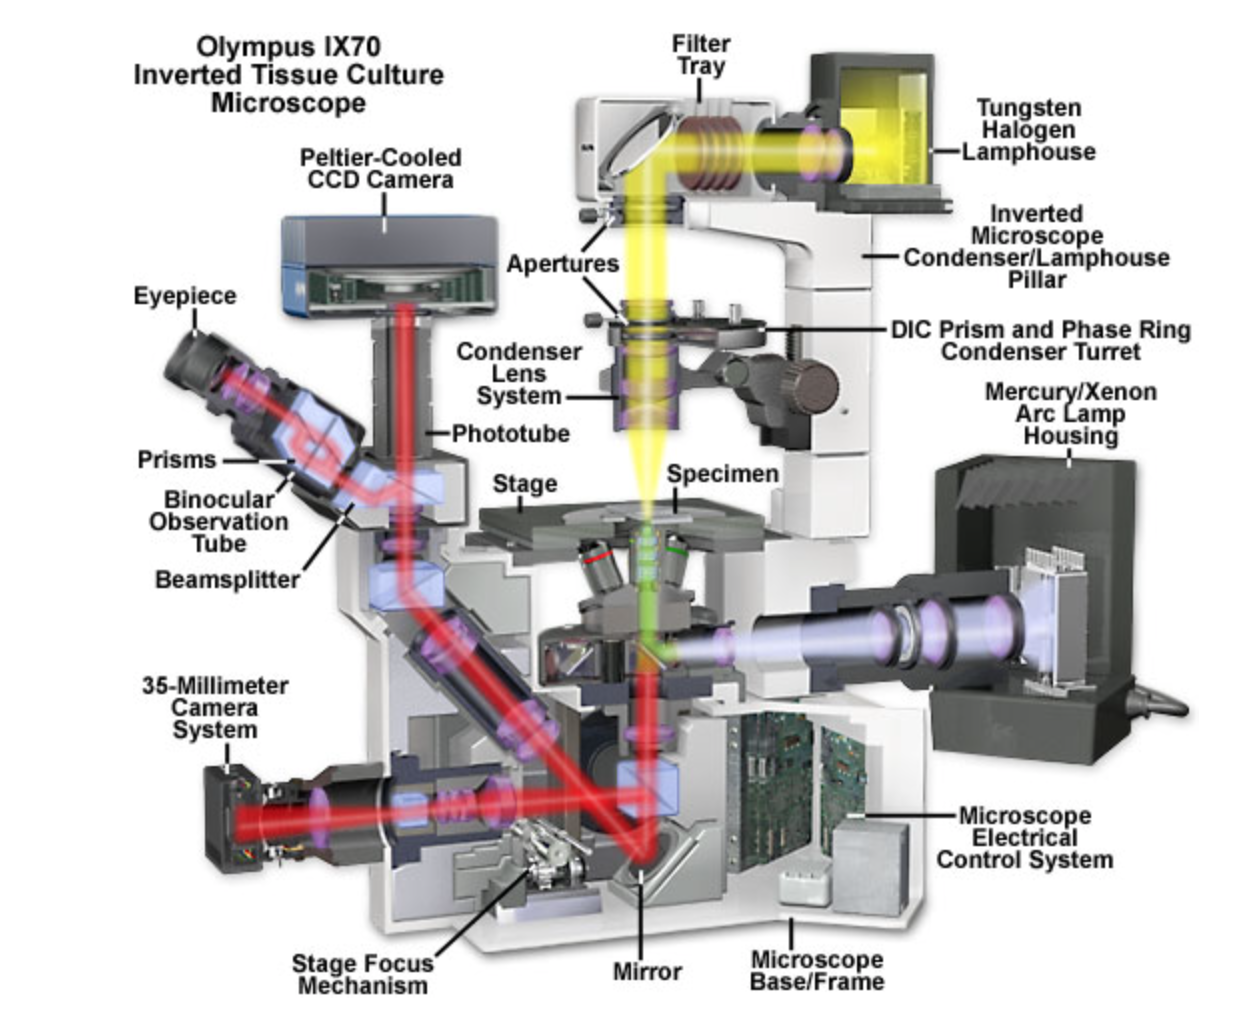
\includegraphics[scale=0.5]{Microscopeinvertedtrain.png}
    %\caption{Components of an inverted microscope. Contrary to a standard microscope, the inverted microscope possesses its illumination system above the stage and their movable microscope objectives. Moving the microscope objective changes the plane of focus captured by the Camera. Image taken from \cite{FluorescenceM}}
    %\label{Microscope inverted}
%\end{figure}
\noindent
%The microscope objective is the closest element of the microscope to the sample, and during the imaging process, it gives feedback to the cameras. In an optical tweezer, the microscope objective images the sample and produces the trap. 

\section{Optical tweezers.}
Optical tweezers are devices that can contactless manipulate, hold and push small
objects of size ranging from the atomic to the micrometric scales \cite{jones2015optical}. It consists of a tightly focused laser beam  (for more on laser functioning and properties, see Appendix A).  Commonly, optical tweezers  are achieved by overfilling a high-numerical
objective lens. The very first theoretical treatment by Ashkin of the force exerted
by a laser beam onto a small dielectric particle was based on the fact that a photon
carries momentum and considered the particle a perfect mirror \cite{jones2015optical}. In this elementary model, a photon reflected perpendicularly to the mirror produces a recoil force onto the last due to the momentum exchange. According to this treatment, when a particle is subjected to a laser beam, a force appears, pushing the particle in the propagation direction of the radiation (scattering force). %This force would push the particle towards the propagation direction of the radiation.
%By conservation of the total momentum of light and mirror, this implies that the mirror experiences an equal and opposite recoil force in the propagation direction of the light.
Additionally, during the experiments, Ashkin observed the existence of an additional transversal component of the
force (gradient force) produced by the radiation onto the paricle \cite{ashkinhistory}. This force would push the particle towards the region of maximum intensity of the laser beam.\\ Indeed,  the interaction between light and a dielectric particle produces a momentum
exchange between them, and the magnitudes and direction of these forces can be computed depending on the size of the particles relative to the wavelength of the laser
beam. Depending on this relationship, we devise three regimes to compute these forces \cite{jones2015optical}: The Lorenz-Mie, the Rayleigh, and the Ray optics regime (for a more detailed review of these regimes, see Appendix B).
%Then Microscope, then Trapping. Then, probably laser light and Gaussian beam. 
%Diatoms are single photosynthetic algal cells populating the oceans and waters
%around the globe. They generate a considerable fraction (20–30%) of all oxygen from photosynthesis,
%and 45% of total primary production of organic material in the sea.


%\subsection{Lorenz-Mie regime.}
%The generalized Lorenz-Mie theory, provides a complete way to calculate these forces \cite{jones2015optical}. However, the situation becomes complex for non-spherical or non-homogenous particles. For most optical trapping experiments, the calculations with this regime become complicated. 

%\subsection{Rayleigh Regime}
%When the particle subjected to the laser beam is much smaller than the wavelength $\lambda$, it is treated as a dipole in an electric field. The trapped particle will feel a conservative force confining it in the high intensity region of the focused laser beam (Gradient force). A non-conservative force (scattering force) will arise due to the transfer of momentum from the field to the particle. This force points in the laser propagation direction and results from the trapped particle's scattering and absorption of photon processes.
%\subsection{Ray optics regime.}
\begin{figure}[H]
    \centering
    \subfloat[\centering ]{{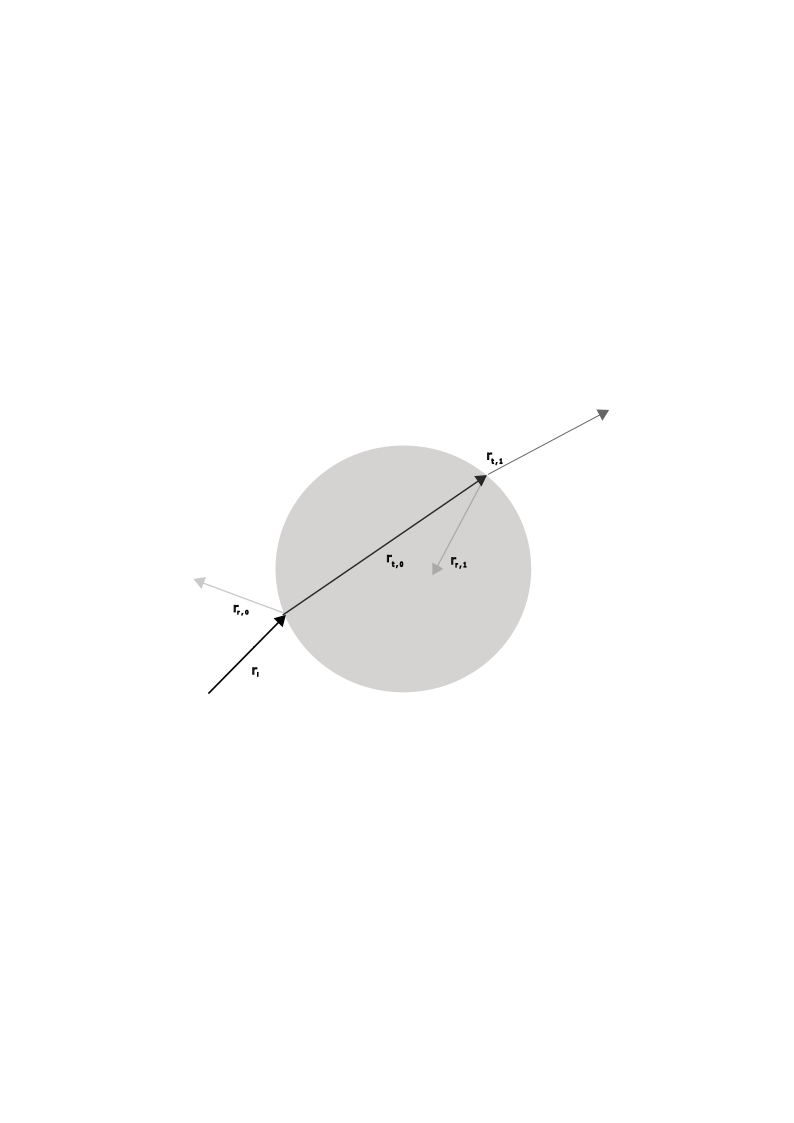
\includegraphics[trim ={2.1cm 9.2cm 2cm 5cm}, scale=0.5]{beadrayoptics.png} }}%
    %\qquad
    \subfloat[\centering]{{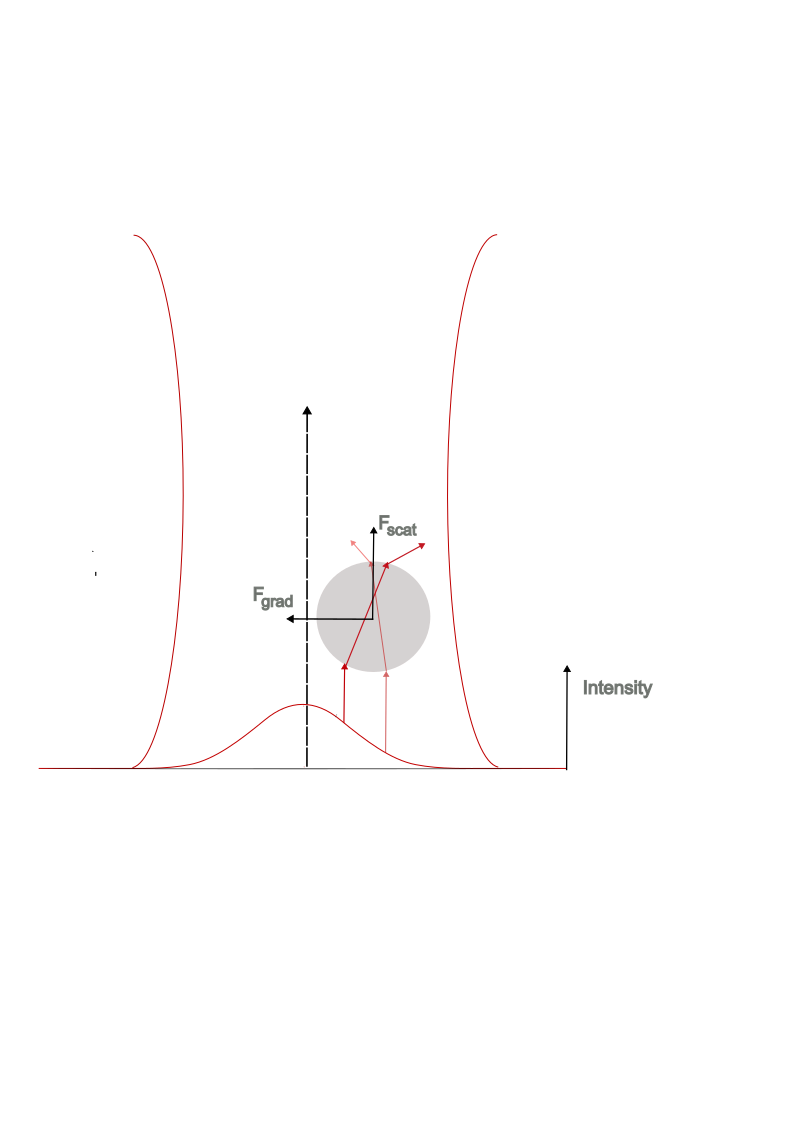
\includegraphics[trim={0cm 7.5cm 2cm 5cm },scale=0.4]{Imagenes teoria/Optical tweezer diagrams/finallyopticaltweezer.png} }}%
    \caption{Ray optics description of the interaction between light and matter in optical tweezers. (a) An incoming ray $r_i$ hits the surface of a spherical bead. From this scattering interaction, we will have a transmitted and a reflected component ($r_{r,0}$ and $r_{t,0}$) of the ray light. The transmitted ray $r_{t,0}$ will undergo another scattering process, producing a new pair of ray beams ($r_{t,1}$ and $r_{r,1}$); the scattering process inside the sphere will continue until all light has escaped from the sphere. Virtually all light has escaped from the sphere within less than 10 scattering events \cite{jones2015optical}. \newline (b) A spherical transparent bead subjected to a Gaussian laser beam. The light intensity distribution forms a Gaussian shape. The bead is off the symmetry axis of the laser beam. Therefore, the force produced by the ray at the left will be stronger than the one by the right ray due to a larger number of photons (higher laser intensity) for the first. The figure shows the forces acting on the bead due to the laser beam $F_{grad}$ and $F_{scat}$. 
 }%
    \label{opticaltweezerfunctioning}%
\end{figure}
\noindent When the particle subjected to the laser beam is much bigger than the wavelength $\lambda$, a ray optics treatment can give a good description of the arising forces. The gradient force and scattering forces mentioned can be described with refraction and reflection laws for light rays traveling through media with different refraction indices (see figure \ref{opticaltweezerfunctioning}).

\noindent In figure \ref{opticaltweezerfunctioning} (b), a simple model is shown. The transmitted rays from the scattering process between the laser beam and the bead will define a plane in space \footnote{The incident, reflected, and refracted light beams are coplanar.}. The force (due to the momentum exchange between the bead and the laser beam) on the sphere lies in this plane and can be decomposed into the scattering ($F_{scat}$) and the gradient force ($F_{grad}$). As seen in the figure, more photons are near the center of the beam, producing a net force pushing the bead towards it (gradient force). Additionally, the scattering force will push the particle in the direction of the beam.\\ \noindent
In practice, calculating the optical force exerted by a focused laser beam requires decomposing the electromagnetic field of the beam into a collection of individual light rays. The \textit{Optical Tweezers in Geometrical Optics} (OTGO) software facilitates this process by enabling the computation of optical forces acting on a dielectric sphere, based on the specific parameters of the experimental setup \cite{callegari2015computational}. 
For a spherical silica particle with a diameter of \(6.59 \, \mu\text{m}\) subjected to a \(532 \, \text{nm}\) laser beam operating at \(120 \, \text{mW}\), the OTGO software provides a visualization of the optical forces acting on the sphere (see figure \ref{OpticalforcessetupKaren}).
\begin{figure}[h]
    \centering
    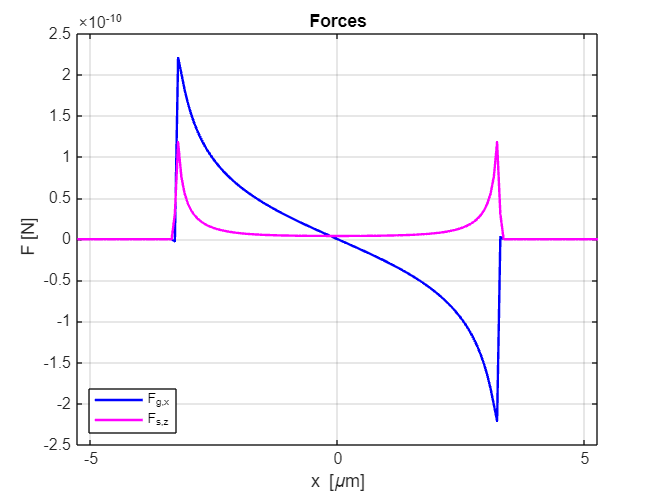
\includegraphics[scale=0.5]{Screenshot 2025-03-05 004832.png}
    \caption{Optical forces $F_g$ and $F_s$ (Gradient force and scattering force respectively) on a $6.59 \mu m$ spherical $SiO_2$ particle produced by a focused laser beam with power set at $120 mW$. The optical forces are computed as a function of the position along the transversal axis x of the trapped particle's center of mass using the OTGO software. The focus of the laser beam in the software is considered to be obtained by overfilling a microscope objective with numerical aperture 1.0 and 60X magnification, as in the experimental set up of this work.}
    \label{OpticalforcessetupKaren}
\end{figure} 
This plot shows the theoretical computation of the optical forces using ray optics for an optical tweezers set up with the mentioned experimental parameters. From the plot it is possible to observe the minute yet significant magnitude of the optical forces occasioned by the laser beam on the silica body. For comparison, the weight of a $SiO_2$ spherical particle with a diameter of $6.29 \, \mu\text{m}$, similar to those employed in this work, is $3.87 \times 10^{-12} \, \text{N}$. This makes the theoretical optical forces two orders of magnitude larger than the weight.
Moreover, we can observe the symmetry of the gradient and scattering forces around the equilibrium position of the trapped particle. As it is expected, the gradient force is a restoring force along the transversal axis x that tends to return the particle to its equilibrium position within the optical trap whereas the scattering force is pushing the particle upwards along the optical axis of the system. This can be seen from the odd and even symmetries of the graphics for the gradient and scattering forces, respectively. 



\newline \noindent In contrast, when the particle is much smaller than the wavelength of the laser, the Rayleigh regime uses electromagnetic theory to describe the forces experienced by the particle in the optical tweezers. 
In this regime, the system of the particle being subjected to the laser beam is approximated as a dipole in an oscillating electric field. When computing the forces of the last system, we find three components of the force: The gradient, the scattering, and the spin-curl force \cite{svelto2010principles}. The gradient force in this model arises from the potential energy of a dipole in the electric field. In terms of the gradient of intensity is \cite{svelto2010principles}
\begin{equation}
    F_{grad}=\frac{1}{2}\frac{\alpha'_d}{c\epsilon_0}\nabla I_i(\mathbf{r_d}),
    \label{gradientforcerayleig}
\end{equation}
Where $\alpha'_d$ is the dispersive part of the polarizability $\alpha=\alpha'_d + i \alpha"$, c is the speed of light and $\nabla I_i\mathbf{(r_d)}$ is the gradient of intensity at the position of the center of mass of the dipole. 
From equation \eqref{gradientforcerayleig}, we can see that particles exhibiting positive polarizability, meaning their refractive index exceeds that of the surrounding medium, tend to be drawn toward high-intensity electric field regions. Conversely, particles with negative polarizability, signifying a refractive index lower than of the surrounding medium, experience repulsion from these high-intensity regions. Additionally, the scattering force appears from the transfer of momentum from the field to the particle as a result of the scattering and absorption processes, and it points in the direction of the Poynting vector $\mathbf{S_i}$ (the direction of the field propagation). Finally, the spin-curl force emerges from polarization gradients in the electromagnetic field. This force is relatively small compared to the previously mentioned, and if the field is homogeneously polarized, it does not appear \cite{jones2015optical}. Usually, it does not play a major role in optical trapping experiments.
\\ In the intermediate regime (the particle dimensions are comparable to the wavelength), rigorous solutions of Maxwell’s equations are required for the system. The Generalized Lorenz-Mie theory fully describes the forces involved in optical tweezers, with a complete wave-optical modelling of the particle–light interaction for particles of any shape and size. It describes such forces using electromagnetic scattering theory \cite{jones2015optical}. In particular, the generalized Lorenz-Mie theory provides the analytical solution for the case of a homogeneous spherical particle. However, the equations become more complex for non-homogeneous and non-spherical particles, and a computational approach could be necessary to find the solution. 


\noindent As we have seen, the relation between the laser beam wavelength and the particle size determines the approach to compute the forces in the optical tweezers. It is important to notice that the wavelength of the laser beam used for the optical tweezers can be selected depending on the application and changed if needed. On the other hand, the particles to be studied are often of a fixed size provided by their mere nature. This is usually the case with biological entities such as viruses and cells or physical particles such as atoms. In particular, the particles trapped in this work range in the micrometer scale, and a sample was prepared to conduct the trapping experiments. A sample is typically made of particles suspended in a liquid restrained with two glass covers. %Similar to what is shown in figure \ref{samplewater}
%\begin{figure}[H]
 %   \centering
%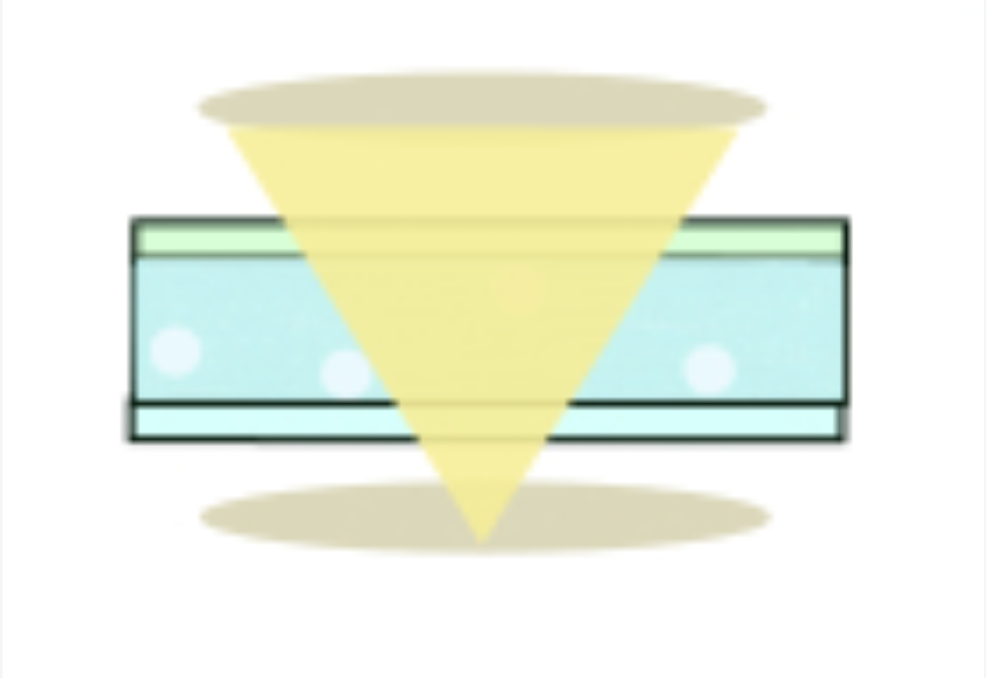
\includegraphics[scale=0.6]{Screen Shot 2023-08-24 at 12.24.32 AM.png}
    %\caption{A typical sample consisting of two glasses containing a liquid with particles floating around. The top lens(grey) is the condenser lens collecting the sample to bath the sample with. Underneath the sample there is the objective lens imaging the sample and producing the optical tweezer by focusing laser light.}
    %\label{samplewater}
%\end{figure}
If, for the application, it is desired to have changes in the suspension media or to control it, a microfluidic device can be used.  %aquí se puede agregar pie de pagina poniendo que tambiåen da una forma de medir fuerzas de manera experimental.

\section{Microfluidics}
A microfluidic device or microfluidic chip is a system designed to handle and manipulate small quantities of fluids on the micrometer scale or below. It is composed of a network of microchannels that can be interconnected to one another (see figure \ref{microfluidic_device}). In these microchannels,
the traveling liquid can be precisely controlled, allowing a stable environment in
experiments where factors such as temperature, pressure, and chemical concentrations should be strictly regulated. Moreover, the microfluidic chip provides for a continuous flow of fluid and refill in case of evaporation or even the exchange of one fluid with another.
 \begin{figure}[H]
     \centering
     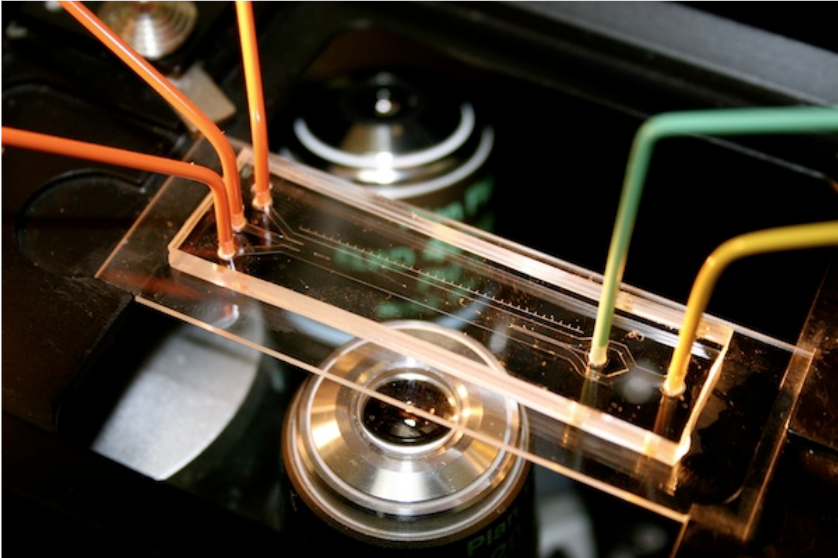
\includegraphics[scale=0.35]{microfluidicinaction.png}
     \caption{A microfluidic device placed on the stage of an inverted microscope. This set-up allows visual tracking of the phenomena happening in the microchannels since the microscope objective images the insides of the microchannels. Image taken from \cite{Wanucha_2012} with permission from the authors.}
     \label{microfluidic_device} .
 \end{figure}
  In figure \ref{microfluidic_device}, we can observe delivery pipelines installed in the microfluidic chip. These pipelines feed the microchannels with the fluid under study using different techniques, such as pressure-driven flow and electrokinetics. Additionally, these techniques provide acceleration of the fluid and controlled manipulation.\\
 The microfluidic device can be made of different materials, including silicon, glass, PDMS, and metals, providing diverse physical properties to the chip
 \cite{Liu2008}.
 The choice of material depends on different factors, including the intended application. This aspect of microfluidic devices allows extensive functionalities and applications, and it is complemented by the variety of designs for the channel network (see figure \ref{simple design} for a simple design of a microfluidic chip) and its low sample consumption.
 \begin{figure}[H]
     \centering
     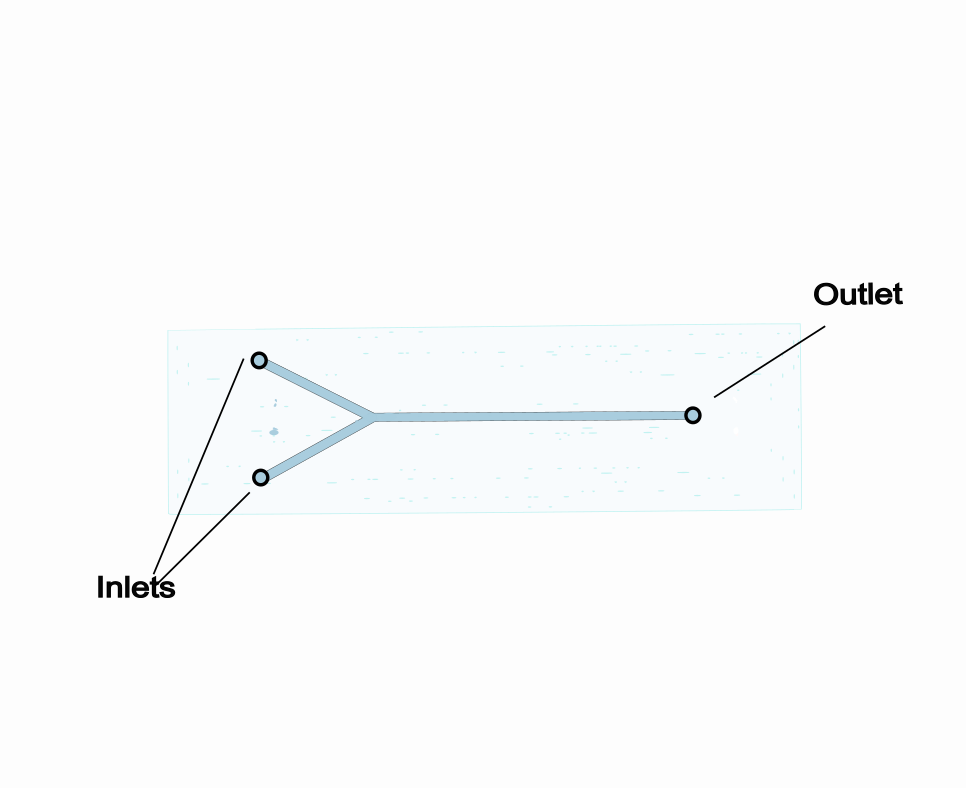
\includegraphics[trim = {0 1.5cm 0 0.7cm}, scale=0.4]{Diatomsexperimentalmethods/Microfluidics designs/Screen Shot 2024-01-17 at 5.34.18 PM.png}
     \caption{A Y-type microfluidic device. With two inlets and one outlet, this design is helpful for mixing micro fluids and microreactor applications \cite{niculescu2022review}. }
     \label{simple design}
 \end{figure}
 %, and provides extensive functionalities to the device. 
 
The attributes of microfluidic devices make them a powerful tool for research in areas where small volumes of liquids and micrometer particles play a significant role. In particular, microfluidic devices find applications across a broad spectrum of fields, including biology (e.g., DNA analysis and cell sorting \cite{wang2011enhancedmicroandopti,paegel2003microfluidicDNA}), chemistry (e.g., synthesis and analysis of chemicals \cite{niculescu2022review}), and physics (e.g., fluid dynamics studies.).\\ In fluid dynamics, understanding the forces acting on particles within these devices is crucial. Specifically, the force exerted on a spherical particle in a microfluidic channel due to a viscous fluid can be computed using Stokes' law, which is valid for low Reynolds number flows, such as the liquid flows that are typical in microfluidics. For a spherical particle of radius \( r \) moving with a velocity \( \mathbf{v} \) in a fluid of dynamic viscosity \( \mu \), the drag force \( \mathbf{F}_d \) is
\begin{equation}
    \mathbf{F}_d = 6 \pi \mu r \mathbf{v}.
\end{equation}

 
\chapter{Experimental methods}
This chapter describes the experimental set-up and the methods used to perform the experiments of this work. 
\section{Microscope and image acquisition.}
A Nikon TE300 Eclipse, a multiport inverted microscope, was used in this study due to its availability in the laboratory. This microscope also features a compartment beneath the rotary objective tray, allowing the insertion of a filter or dichroic mirror to modify the incoming light from the objective. A 60x water immersion microscope objective manufactured by Nikon with numerical aperture $NA=1.00$ and working distance $WD=2$ mm; and a 100x oil immersion Nikon Microscope objective with numerical aperture $NA=1.40$ and working distance $WD$ of 0.13 mm facilitated the imaging of the samples placed in the microscope's stage. Additionally to the eyepiece, the TE300 eclipse microscope possesses a side port and a front port to attach camera systems to the microscope. In each port, an Axis m1103 camera was placed to transmit the image of the sample to a computer. The data transmission between the camera and the computer is facilitated by utilizing a secure LAN connection linking the two devices. An NF533-17 notch filter was placed in front of the cameras' apertures, preventing the high-intensity radiation from the laser device from reaching the cameras' sensor. Additionally, another NF533-17 filter was installed in the microscope eyepiece compartment for filters. The TE300 microscope possesses a knob to move the microscope objective in the vertical direction. 
A stage controller joystick enabled the adjustment of the position in the xy plane of the stage, facilitating the examination of different areas of the sample.
\newpage
\section{Optical tweezers.}
Figure \ref{setuptweezers} shows a schematic for the optical tweezers set-up.  
\begin{figure}[H]
    \centering
    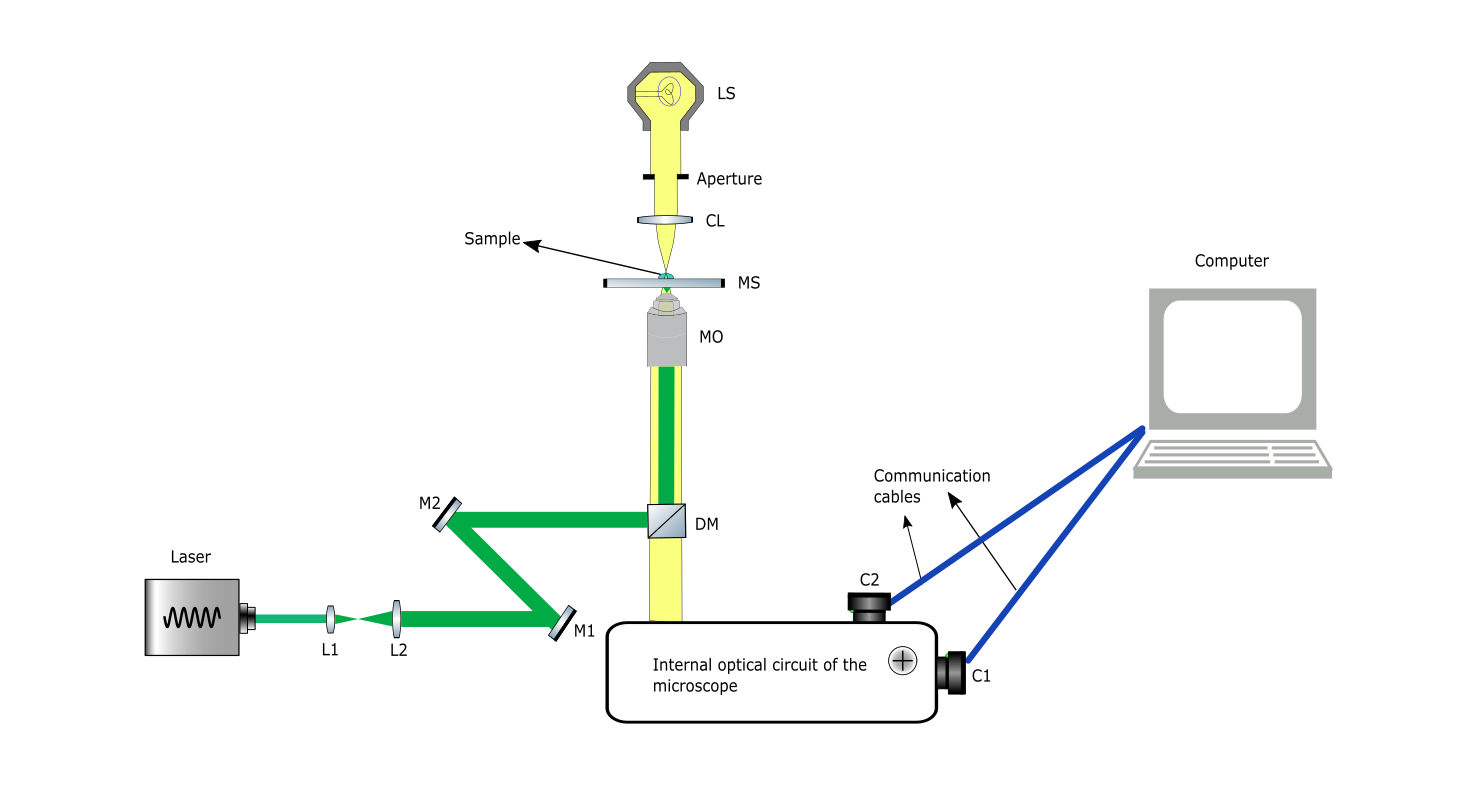
\includegraphics[scale=0.40]{Newplots_microfluidics_results/setup3.png}
    \caption{Standard set-up for optical tweezers. A laser device facilitates the radiation to produce the optical trap. $L_1$ and $L_2$ are two positive lenses with focal lengths $f_1$ and $f_2$, respectively. These lenses are placed at a distance $f_1 +f_2$ between each other, expanding the laser beam to overfill the back aperture of the microscope objective (MO). $ M_1$ and $M_2$ are mirrors for aligning the laser beam. By steering these mirrors, the focus position of the transmitted beam coming out from the microscope objective will change, making possible to move the trapping position of the optical tweezers. The laser light is reflected towards the back aperture of the microscope objective lens (MO) by a dichroic mirror (DM). The microscope objective focuses the incoming laser beam onto the sample, which is placed on a microscope slide in the sample stage. Regarding the imaging process, the illumination source (LS) from the lamphouse is adjusted by an aperture before reaching the condenser lens (CL) to ensure the sample is uniformly illuminated. The microscope objective then captures the light refracted by the sample and transmits it into the microscope's internal optical system. The microscope is equipped with a knob that allows the user to switch the output port of the light, directing it to either Camera 1 (C1) or Camera 2 (C2), depending on the selected output channel. These cameras are connected through a communication channel to the computer, where we can record and visualize the trapping experiments.}
    \label{setuptweezers}
\end{figure}
The set-up used to perform the experiments in this work employed a 532 nm CW linearly polarized laser (Laser Quantum gem 532). The intensity was controlled from a computer with the Laser Quantum RemoteApp Laser Control software provided by the manufacturer. The output diameter of the laser beam (0.9 mm) was expanded with a system of two positive lenses, as shown in figure \ref{setuptweezers}. The lens system ($L_1$ and $L_2$) was changed throughout the experiments to adjust the overfilling of the microscope objective back aperture, bearing different trapping performances for the optical tweezers. In particular, the lens systems employed had the following focal lengths configuration ($f_1$, $f_2$): (20 mm, 40 mm), (20 mm, 100 mm), and (20 mm, 200 mm). These lens configurations form a 2 times, a 5 times, and a 10 times magnification beam expander, respectively. The optical tweezers were also implemented with a setup that did not include a beam expander (i.e., no lens system to expand the laser output beam). Broadband mirrors (corresponding to $M1$, and $M2$ in figure \ref{setuptweezers}) were used to align the laser beam. The alignment of the laser beam producing the optical tweezers is important for the trapping performance. A good alignment consists of an incoming laser beam parallel to the optical axis of the microscope objective. 
Symmetrical back-scattered radiation patterns are produced in this case, when the focused laser beam exciting the MO reaches the surface of the microscope slide containing the sample (see figure \ref{symmetricpattern}). 
%Backscattered pattern two figures.
\begin{figure}[H]
    \centering
    \subfloat[\centering]{{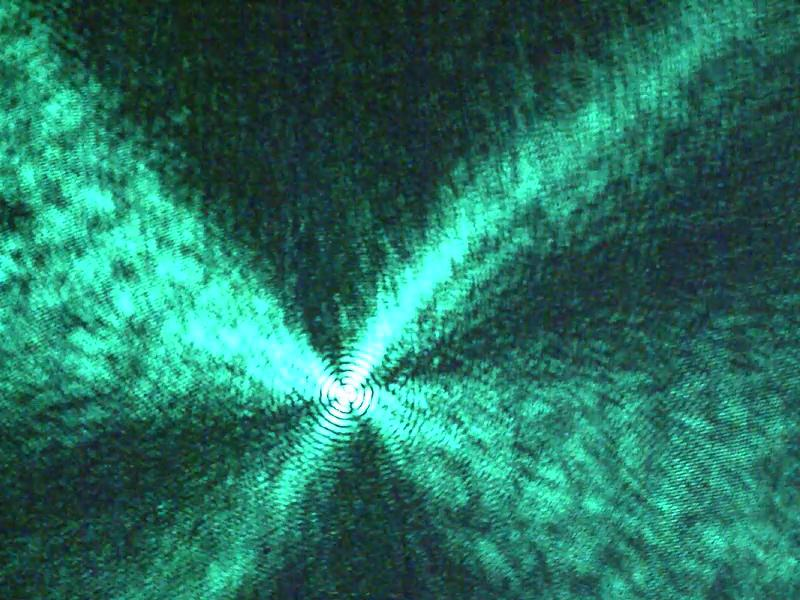
\includegraphics[scale=0.12]{Diatomsexperimentalmethods/Backscateringpattern/backscattered.jpeg} }}%
    \qquad
    \subfloat[\centering]{{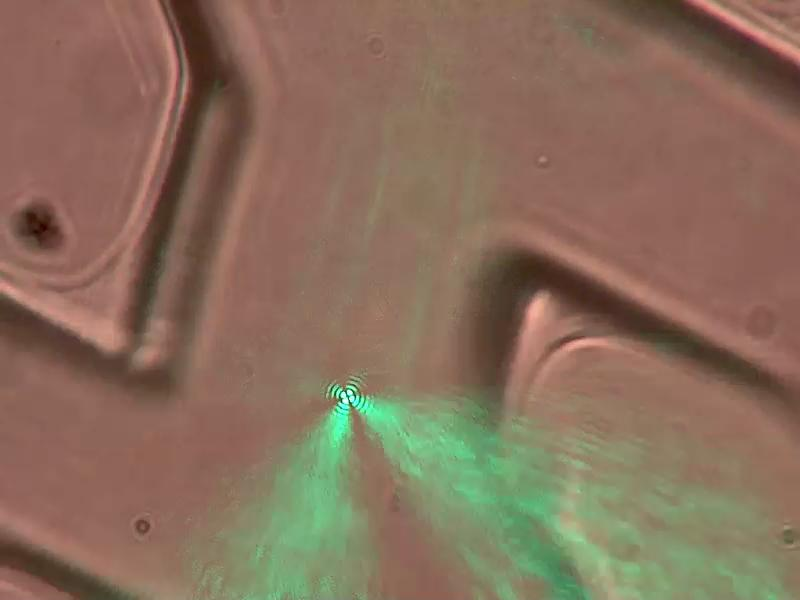
\includegraphics[scale=0.12]{Diatomsexperimentalmethods/Backscateringpattern/inmicrofluidics.jpeg} }}%
    \caption{Back-scattered light patterns captured with the Axis M1103 camera. The water immersion microscope objective was used to focus the laser light in both figures.  (a) Back-scattered radiation pattern produced from a microscope slide with no sample on it.  (b) Back-scattered radiation pattern observed through the microfluidic device used in this work. The centre of this pattern points at the trapping location of the optical tweezers. The back-scattered radiation pattern is a function of the distance between the cover slide interface and the focal point(where the laser beam converges after the MO). The symmetry of the pattern should remain when changing the focus-interface distance.   }%
    \label{symmetricpattern}%
\end{figure}
Steering the mirrors $M_1$ and $M_2$ moves the back-scattered radiation pattern to different locations on the camera and causes its shape to change. Consequently, the symmetry is not necessarily maintained, as the angle of incidence of the incoming laser beam is affected by the steering mirrors. Furthermore, adjusting the position of the microscope objective along its optical axis using the microscope's knob changes the focus-glass interface distance. These capabilities allow for the visualization of the back-scattered pattern of the laser beam as it reaches the glass interface from various angles, facilitating the alignment of the laser beam when symmetry was observed in the pattern.\\
In regard to the 3D manipulation of the particles subjected to the previously aligned laser beam, along with a rotary nosepiece that can move vertically, the Nikon TE300 microscope features a horizontally movable sample stage. These features allowed for the 3D manipulation of the particles using the setup. \\
In particular, this work used a polarizing beam splitter (CCM1-PBS25-532) instead of a dichroic mirror to redirect the incoming laser light toward the back aperture of the microscope objective in the setup.  
As showcased in the theoretical background chapter, the objective lens (MO) is the most critical component of the optical tweezers and the microscope. The two microscope objectives mentioned before were employed to produce the optical tweezers and visualize the sample during the experiments. %: The first one was a 60x water immersion microscope objective manufactured by Nikon with numerical aperture $NA=1.00$ and working distance $WD=2$mm, and the second one was a 100x oil immersion Nikon Microscope objective with numerical aperture $NA=1.40$ and working distance $WD$ of 0.13 mm. These microscope objectives were mounted onto an inverted Nikon Eclipse TE300 microscope. 
In the Nikon TE300 microscope, the condenser lens focuses the light that comes from the lamphouse onto the sample. This ensures that the sample is evenly and adequately illuminated for observation. The condenser lens and lamphouse are positioned above the sample stage, similar to the design of the Olympus IX70 microscope.

\\ \noindent The beam splitter used to redirect the laser light towards the back aperture of the MO also transmitted the refracted light by the sample towards the inner optical circuit of the microscope, producing the image of the trapped particle in the sample. The pair of AXIS M1103 cameras and the incorporated eyepiece of the microscope were used to visualize the trapping of the particles with the optical tweezers. 
%It is important to point out that filters were placed in front of the cameras and the eyepiece to avoid direct collection of the laser beam light. 

\section{Sample preparation and microfluidics.}
Different silica bodies were employed in this work. Artificial spherical $SiO_2$ particles were used to test the trapping capability of the optical tweezers constructed throughout this work. In particular, silica particles of diameter $24.82\mu m$, $19.98 \mu m$, $6.59 \mu m$, and $4.27 \mu m$ were employed. These $SiO_2$ bodies were previously contained in aqueous suspensions with a concentration of $2.5\% w/v$, where the weight-per-volume percentage ($\% w/v$) represents the mass of the solute divided by the solution's volume, expressed as a percentage.
In addition, different species of diatoms were studied in this work (see figure \ref{DiatomExperiments}).
 \begin{figure} [H]
\centering
\begin{tabular}{cccc}
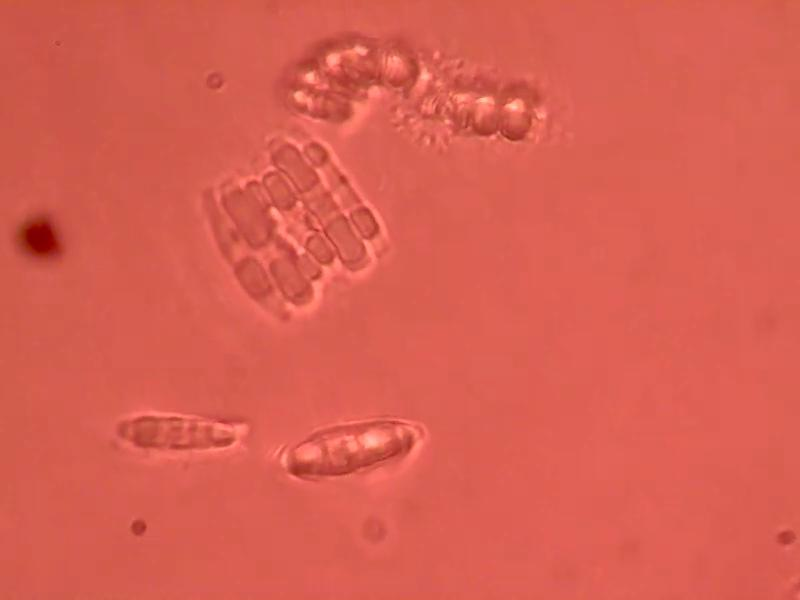
\includegraphics[width=0.3\textwidth]{Diatomsexperimentalmethods/Nitzchia sp1.jpeg} &
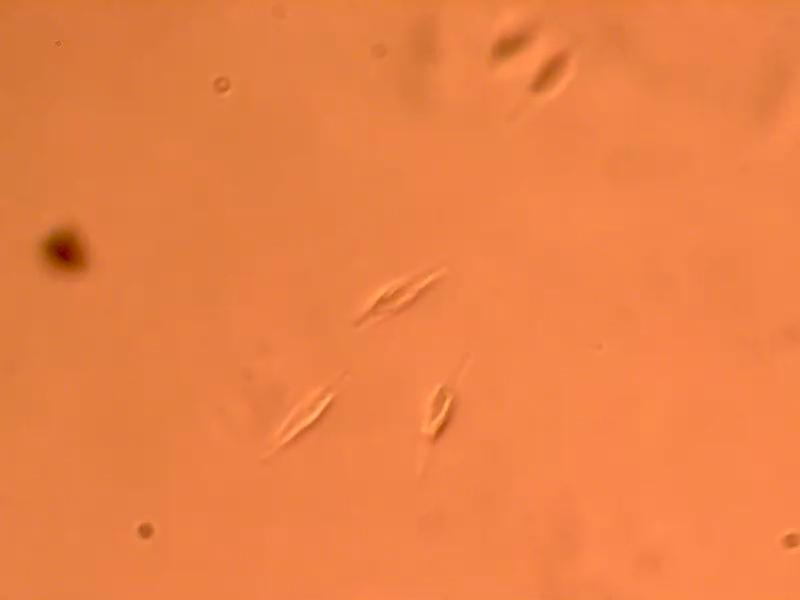
\includegraphics[width=0.3\textwidth]{Diatomsexperimentalmethods/Phaeodactylum t.jpgss.jpg} &
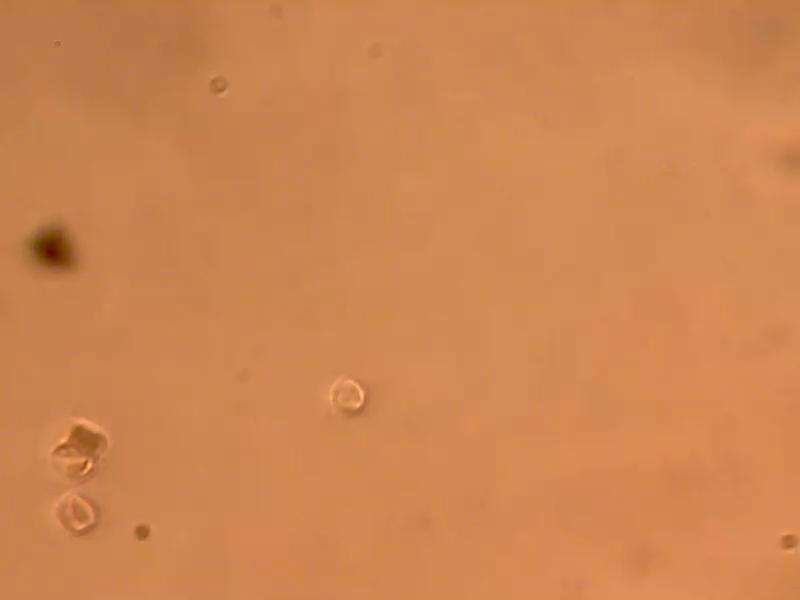
\includegraphics[width=0.3\textwidth]{Diatomsexperimentalmethods/thala2.jpeg} \\
\text{(a) }  & \text{(b)} & \text{(c)}  \\[6pt]
\end{tabular}
\begin{tabular}{cccc}
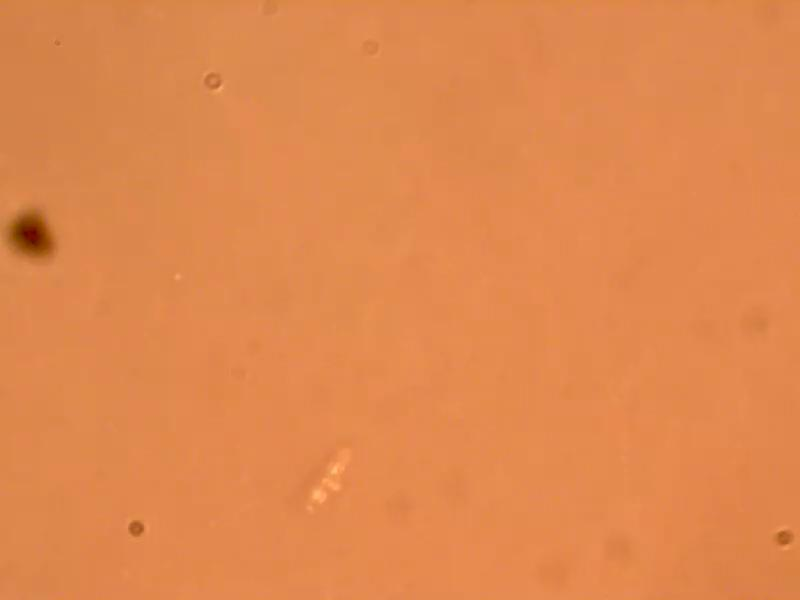
\includegraphics[width=0.3\textwidth]{Diatomsexperimentalmethods/gea4al.jpeg} &
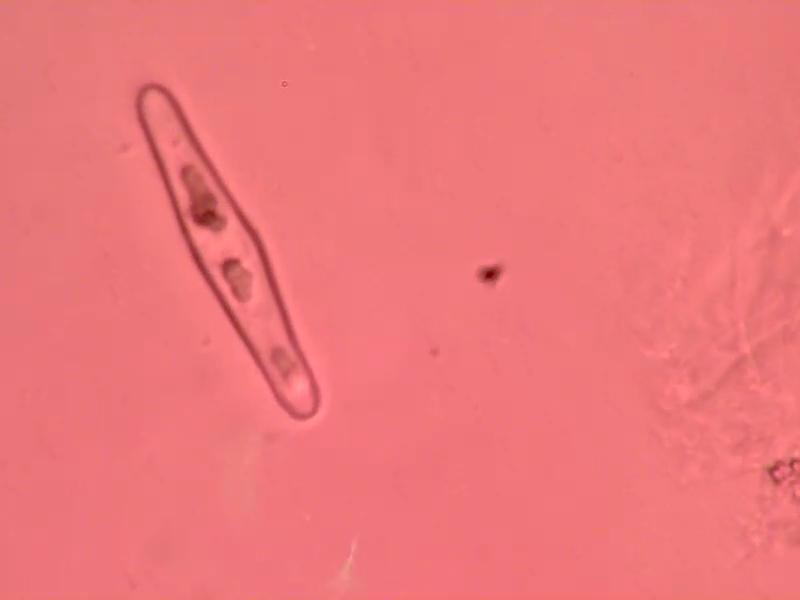
\includegraphics[width=0.3\textwidth]{Diatomsexperimentalmethods/ray.jpeg} \\
\text{(d)}  & \text{(e)}  \\[6pt]
\end{tabular}
\caption{Diatomic algae species studied in this work imaged with the water immersion microscope objective. \text{(a)} Multitude of \textit{Nitzschia sp}.  
\text{(b)} Sample of \textit{Phaeodactylum tricornutum} Diatom species.
\text{(c)} Sample of \textit{Thalassiosira pseudonana} Diatom species.
\text{(d)} \textit{Navicula Sp. 12} Diatom.
\text{(e)} \textit{Marine pennate} Diatom.}
\label{DiatomExperiments}
\end{figure}
A $2\%$ $w/v$ aqueous solution of yeast cells was prepared in addition to the samples of silica particles. 
Regarding sample preparation, for the experiments in which the trapping capability of the optical tweezers was tested, the sample solution (silica particles or yeast cells) was placed on top of a typical microscope slide and covered by a microscope coverslip. To create space between these two glasses, a fence of vacuum grease was used to contain the sample solution pool (see figure \ref{VG}).\\
\begin{figure}[H]
    \centering
    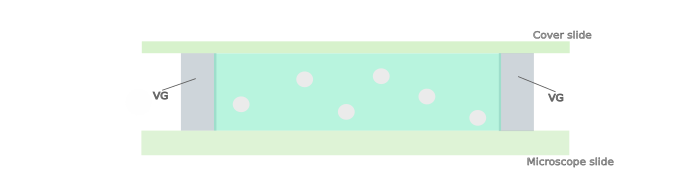
\includegraphics[trim ={1cm 0 0cm 0cm}, scale=.6]{Imagenes teoria/cuci.png}
    \caption{Sample preparation. A vacuum grease (VG) fence contains the aqueous suspensions with the particles to be trapped within the cover and the microscope slides. The sample is placed in the microscope stage, to visualize the particles and test the optical tweezers' trapping capability.}% you need long time for this experiments.
    \label{VG}
\end{figure}
The microfluidic devices employed in this work were made of Polydimethylsiloxane and manufactured at the University of Gothenburg's PDMS lab. The design of the microfluidic chip consisted of three independent channels where the liquid could flow. Each channel featured an inlet and oulet at its ends. Each inlet channel was $100$ $\mu m$ high and $300$ $\mu m $ wide, resulting in a cross-sectional area of $3.0 \times 10^{-8} m^2$ for its transversal profile. This area acts as the conversion factor for transforming flow rates into linear velocities.
%The microfluidic devices used in this study were fabricated from polydimethylsiloxane (PDMS) and manufactured in the PDMS lab at the University of Gothenburg. The microfluidic chip design featured three independent channels for liquid flow. Each channel was equipped with an inlet and an outlet at its ends. The dimensions of each inlet channel were 100 µm in height and 250 µm in width, resulting in a cross-sectional area o
 
The microfluidic devices were placed in the microscope stage, and a CMA 4004 Syringe pump was used to feed the channels with the sample solutions (Diatoms, artificial silica particles, or yeast cells) from a 5ml syringe, and control the flow velocity (see figure \ref{microfluidicsystem} for a diagram of the microfluidic system).
\begin{figure}[H]
    \centering
    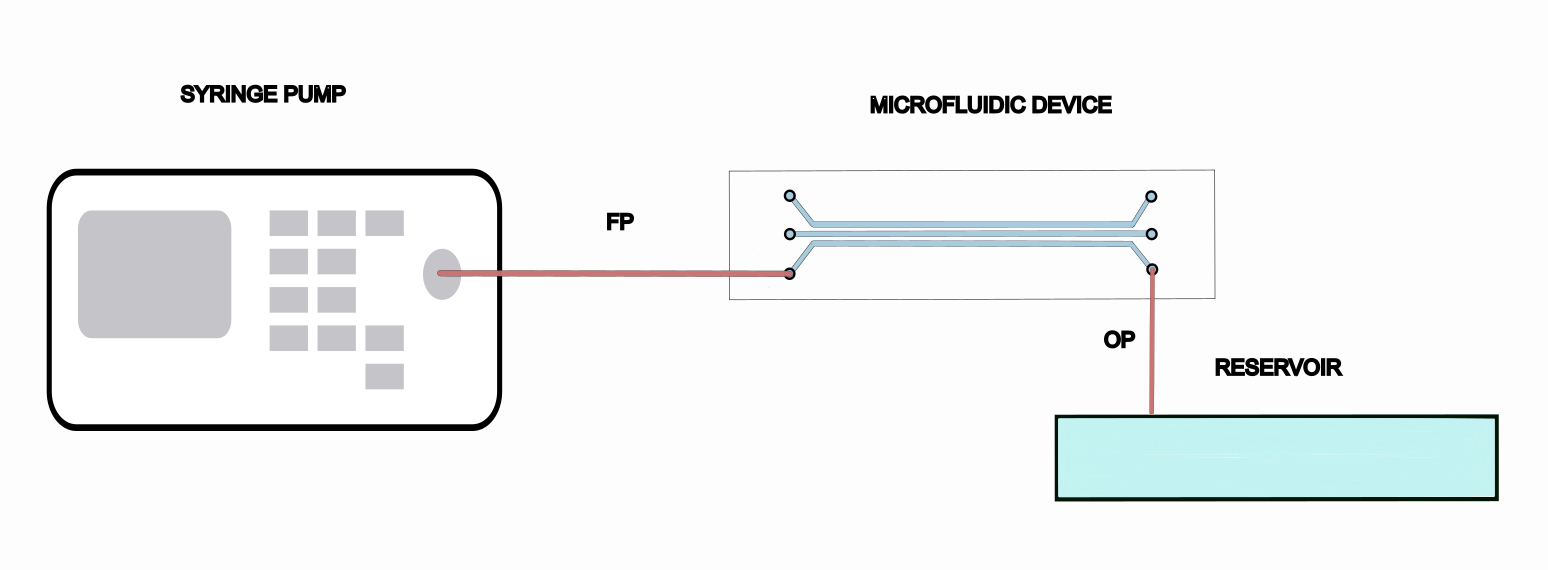
\includegraphics[scale=0.55]{Diatomsexperimentalmethods/Samplepreparation/Screen Shot 2024-01-18 at 12.50.20 PM.png}
    \caption{Schematic of the microfluidic system. The syringe pump controls the flow velocity of the solution entering the channel through the feeding pipe (FP) embedded in the channel inlet. Once the fluid reaches the outlet of the channel, an outlet pipe (OP) directs the effluent solution to a reservoir.}
    \label{microfluidicsystem}
\end{figure}
%The microfluidic device had three independent channels where the liquid could flow.  %In regard to the sample preparation  %On the other hand, different species of Diatoms were studied in this work. In particular, Marine pennet, Nitzchia Sp, Phaeodactylum tricornutum,  Thalassiosira pseudonana, and Navicula Sp were used (see figure).


%In regards to the sample preparation, for the experiments where the trapping performance of the optical tweezers was tested, the sample preparation consisted of a typical Coverslip on top of a microscope coverslide, these two separated by a sample pool contained by a fence of vacuum grease. On the other hand, when using the microfluidic channels, a 
%A microscope Nikon TE300 microscope was used to image and place the sample. Two microscope objectives (Nikon Plan Apo 100x 1.40NA oil immersion and Nikon Fluor water immersion 60x 1.00NA)  were used to converge the laser beam (532 nm gem) in the focal point.
\newline %About microfluidic chips and Diatoms, then aligning, figures of the set-up, and back-scattered radiation pattern.

%\begin{figure}[H]
 %   \centering
  %  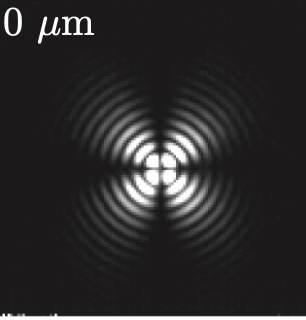
\includegraphics[scale=0.75]{Screen Shot 2022-09-19 at 8.24.26 PM.png}
   % \caption{Back-scattered light pattern from a focused beam. The back-scattered radiation pattern is a function of the distance between the cover slide interface and the focal point. Often, one can observe rings instead [10].
%The symmetry of the pattern should remain when changing the focus-interface distance. Figure taken from [10].}
    %\label{fig:my_label}
%\end{figure}
%\noindent
%During the alignment of the set-up, the following pattern was observed.
%\begin{figure}[H]
 %   \centering
  %  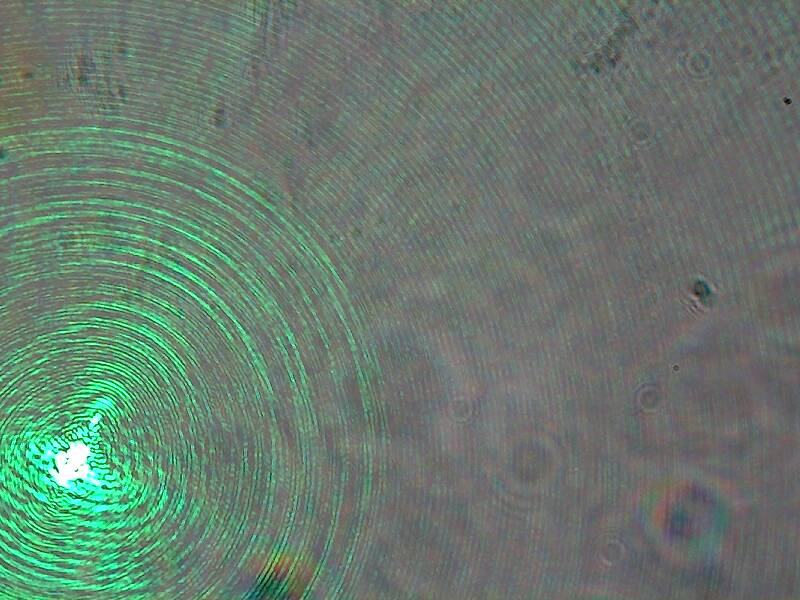
\includegraphics[scale=0.17]{center.jpeg}
   % \caption{Back-scattered radiation pattern. The interference pattern due to the dichroic mirror was observed.}
    %\label{fig:my_label}
%\end{figure}
%\noindent
%The following pattern remained symmetric when moving the focal point in the objective axis. By moving the mirrors $M_1$ and $M_2$ the pattern was moved to the center of the image produced by the camera. However, the particle was not trapped. After realigning, changing the filling of the microscope
%objective, and, trying with different sized particles the problem sources were narrowed down to the camera. Then, a second camera was installed. The same image
%was shown. Therefore, the only source of error was the alignment of the camera's field of view.
%\newline
%To overcome this problem, the alignment was made based on the reflected light of the microscope lamp. \newline 
%\noindent
%With this change, the symmetric pattern disappeared from the camera's field of view. However, 4μm silica particles were
%trapped with both microscope objectives when moving the translational stage slowly. Yet, a high power output of the laser beam was needed. 
%\newline For 4$\mu$m silica particles the trapping was achieved with power from 864.0mw. \\
%Using a powermeter, it was found that the laser power decreased to $10\%$ of the output when reaching the back aperture of the microscope objective.

%\newline
%\noindent
%A compendium of recordings of the trapped particles will be stored in the following drive.
\chapter{Results}
%First option: This chapter presents and discusses the results obtained when performing the experiments with the optical tweezers, and methods presented in Chapter 3. The long-term goal of this project is to produce a comprehensive and exhaustive single-cell study for diatom species assisted with optical tweezers that include the measure of external forces, the effects of changing media, and light sources on their reproduction processes or the integrity of the cell, and the characterization of their photonics properties.

This chapter presents and discusses the results obtained from the experiments conducted with the optical tweezers and the methods presented in Chapter 3. The long-term goal of this project is to produce a comprehensive and exhaustive single-cell study for diatom species assisted with optical tweezers. %borrado despues de iteracion con KV S Lauras master This study will encompass the measurement of external forces, the effects of changing media, and exposure to light sources on the reproduction processes and cell integrity of the diatoms, in addition to the characterization of the optical properties of the frustules.
%This, will allow for the photonical properties uncovering of shit of optical tweezers. %Step furthening
\\ In this regard, each section of this chapter showcases results that mark significant progress toward achieving this long-term goal. In particular, there is a section regarding the trapping of the artificial $SiO_2$ particles with different sizes, and one section is for the trapping and manipulation of different Diatom species, along with the specific microscope objectives and beam expanding systems used for each experiment. Additionally, there is a section for the trapping of the yeast cells and one for the usage of optical tweezers to trap particles in a microfluidic system flow at different velocities. 
\\The whole chapter is written as an evolution towards the mentioned goal. The first logical step was to produce robust 3D optical tweezers. For this matter, the artificial silica particles were employed due to their symmetry and their well-known compatibility for experiments with optical tweezers.

%With this aim in mind, each section of this chapter showcases results that mark significant progress towards achieving this overarching goal.


%With this overarching goal in mind, each section of this chapter highlights results that signify significant advancements towards fulfilling this objective.
%regarding the trapping of the $SiO_2$ particles based on their nature (Diatoms or artificially engineered particles), size or species, and the specific tools used to construct the optical tweezers (beam expanding system, and microscope objective).  Additionally, there is a section for the trapping of the yeast cells and one for the usage of optical tweezers to trap particles flowing through the microfluidic channels at different velocities. 




\section{Manipulation of silica particles}
%The manipulation of the artificial $SiO_2$ was achieved with different beam expander configurations and the water immersion microscope objective. The laser power needed to trap these particles ranged between 12 to 100 $mW$ for all the beam expander setups tried in this work. 
The very first optical tweezers constructed employed a 10x beam expander system and were tested with the 4.27 $\mu m$ $SiO_2$ (see figure \ref{figur427}), and the 19.98 $\mu m$ silica particles.

%4.27 sio2 particles
\begin{figure}[H] 
  \begin{subfigure}[b]{0.5\linewidth}
    \centering
    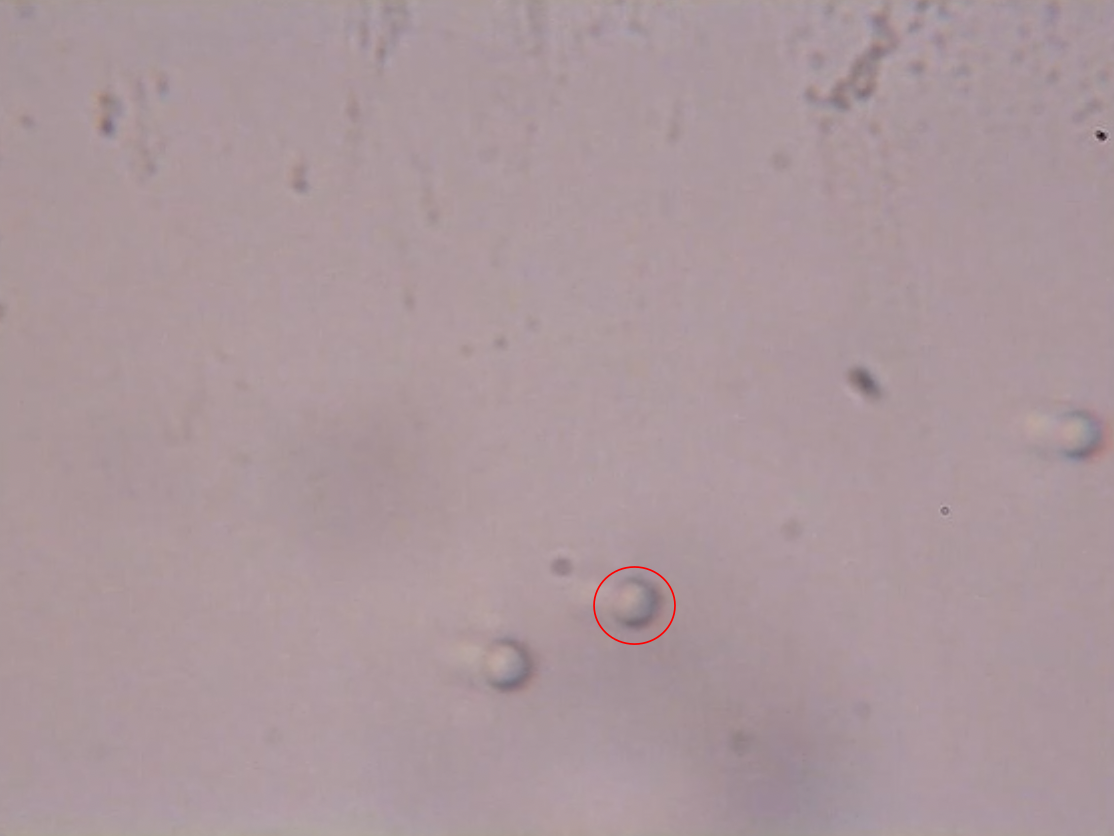
\includegraphics[scale=0.22]{427particles/image732.png} 
    \caption{}
    
    \label{} 
    \vspace{4ex}
  \end{subfigure}%% 
  \begin{subfigure}[b]{0.5\linewidth}
    \centering
    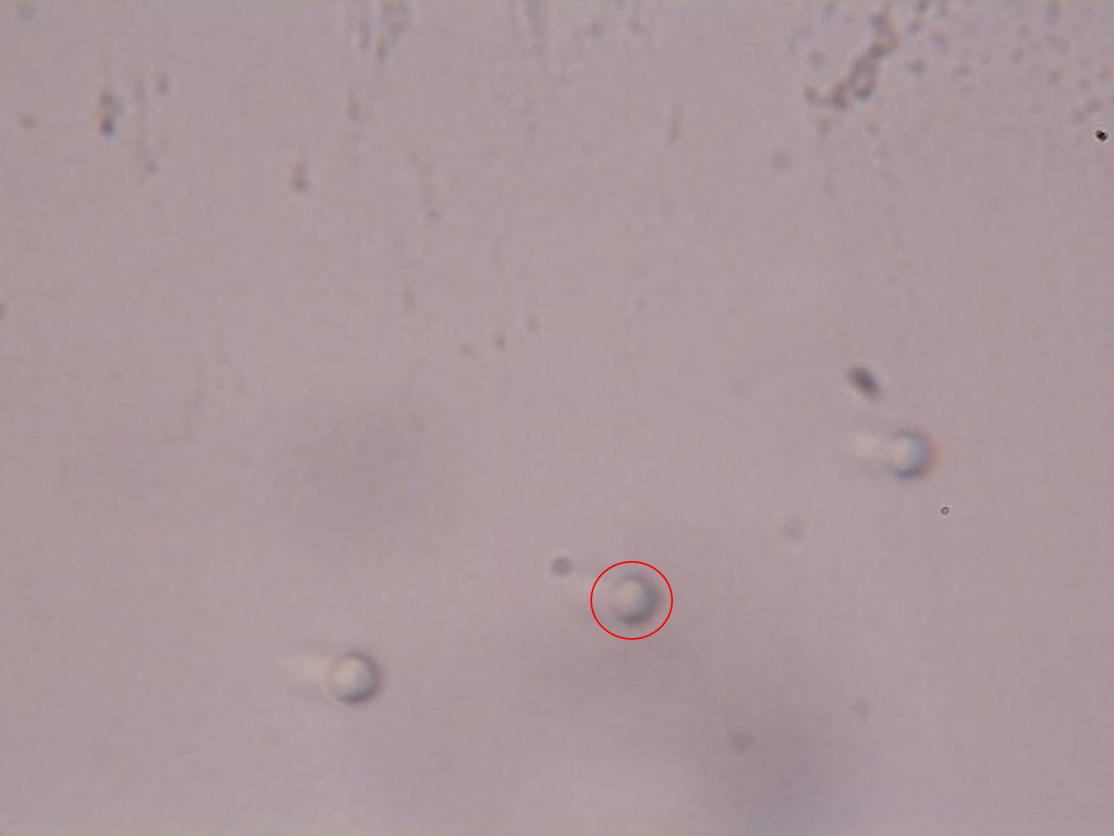
\includegraphics[scale=0.22]{427particles/2.png} 
    \caption{}
    \label{fig7:b} 
    \vspace{4ex}
  \end{subfigure} 
  \begin{subfigure}[b]{0.5\linewidth}
    \centering
    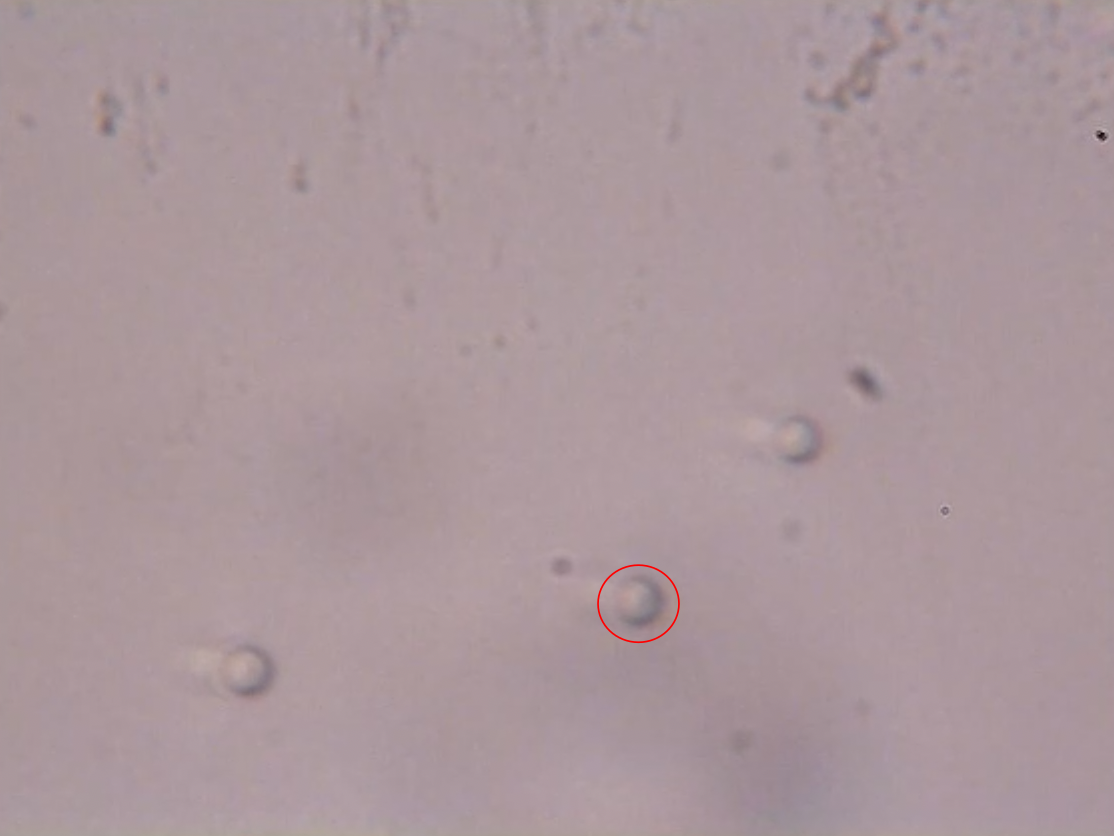
\includegraphics[scale=0.22]{427particles/i.png} 
    \caption{}
    \label{fig7:c} 
  \end{subfigure}%%
  \begin{subfigure}[b]{0.5\linewidth}
    \centering
    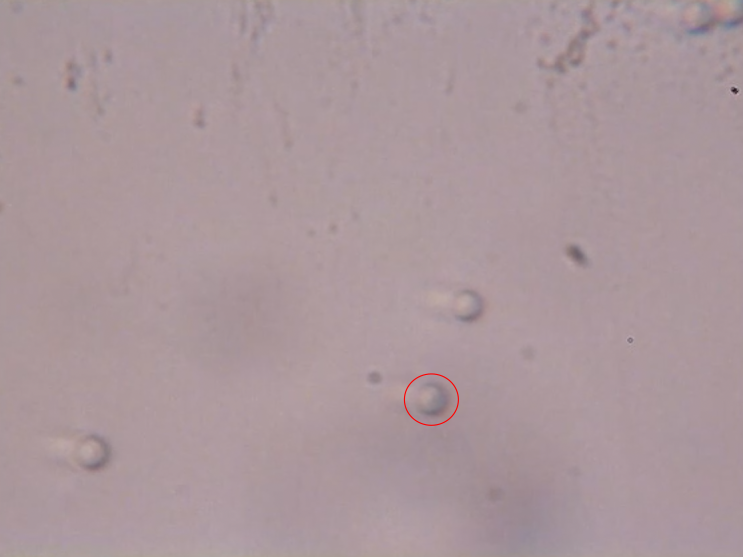
\includegraphics[scale=0.22]{427particles/4.png}
    \caption{}
    \label{fig7:d} 
  \end{subfigure} 
  \caption{Trapping of 4.27$\mu m$ $SiO_2$ particles. Incoming laser power set at 53 $mW$ reaching the back aperture of the water immersion microscope objective with a 10x beam expander. (a-d) The trapped particle (red circle) remains stationary, while the surrounding ones are moved with the stage controller joystick.}
  \label{figur427} 
\end{figure}
However, these optical tweezers did not provide a robust 3D manipulation for the particles above.
%termina aquí las particulas 4.27
The need to improve the performance of optical tweezers to achieve a 3D trap drove the modification of beam expander systems throughout this work. Moreover, it led to refining the alignment of the setup for each configuration. This alignment enhancement allowed for the stable 3D manipulation of the silica particles with the optical tweezers for the 2x, 5x, and 10x beam expander systems. The following images (figure \ref{fig2d}, and figure \ref{fig3d}) illustrate the 2D and 3D manipulation of the 24.82 $\mu m$, and the 6.59 $\mu m$ respectively.
%figuras de la orbita.

\begin{figure}[H]
     \centering
     \begin{subfigure}[b]{0.3\textwidth}
         \centering
         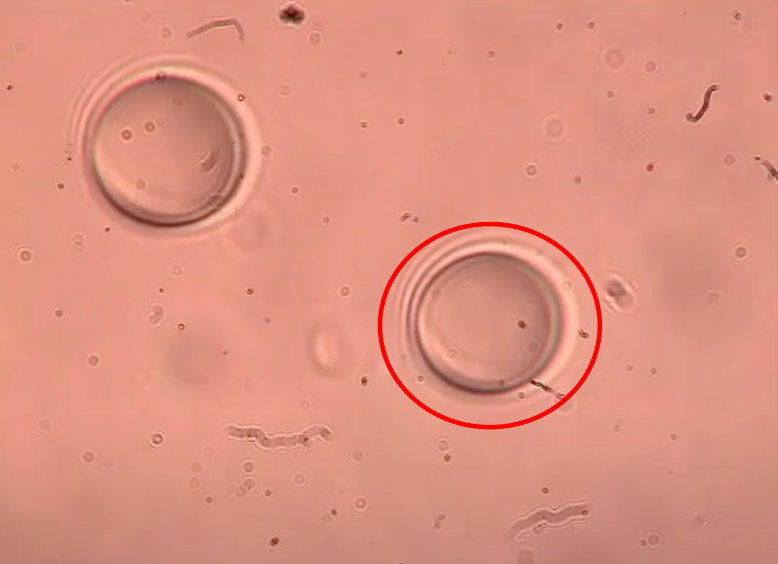
\includegraphics[width=\textwidth]{orbitando2.png}
         \caption{}
         \label{fig:y equals x}
     \end{subfigure}
     \hfill
     \begin{subfigure}[b]{0.3\textwidth}
         \centering
         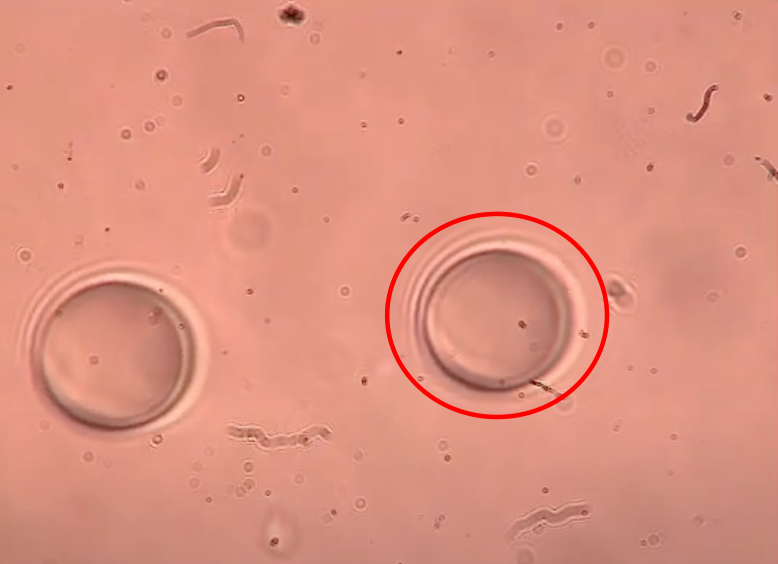
\includegraphics[width=\textwidth]{orbitando3.png}
         \caption{}
         \label{fig:three sin x}
     \end{subfigure}
     \hfill
     \begin{subfigure}[b]{0.3\textwidth}
         \centering
         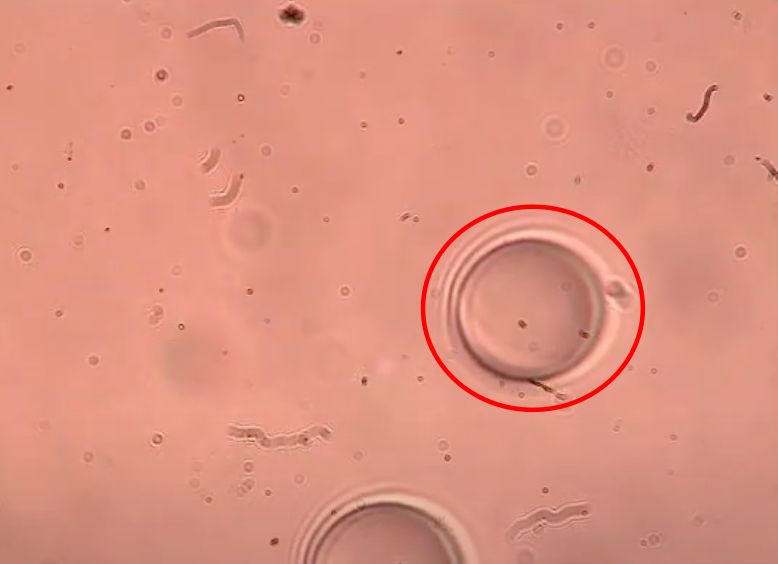
\includegraphics[width=\textwidth]{orbitando4.png}
         \caption{}
         \label{fig:five over x}
     \end{subfigure}
        \hfill
        \\\noindent \centering \begin{subfigure}[b]{0.3\textwidth}
         \centering
         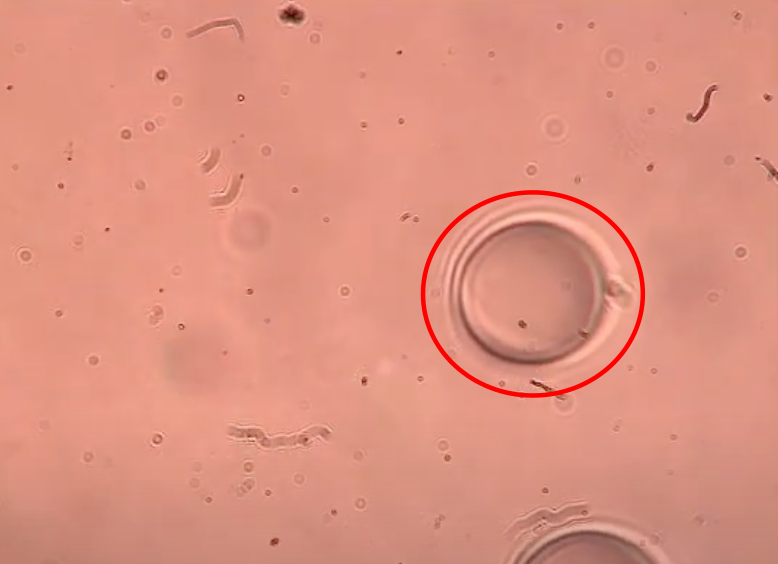
\includegraphics[width=\textwidth]{orbitando5.png}
         \caption{}
         \label{fig:five over x}
     \end{subfigure}
     \hfill
     \begin{subfigure}[b]{0.3\textwidth}
         \centering
         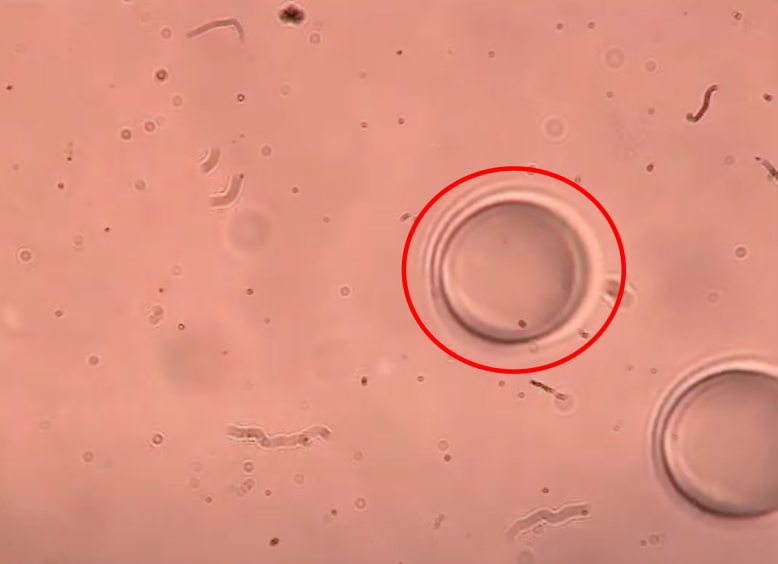
\includegraphics[width=\textwidth]{orbitando6.png}
         \caption{}
         \label{fig:five over x}
     \end{subfigure}
     \hfill
     \begin{subfigure}[b]{0.3\textwidth}
         \centering
         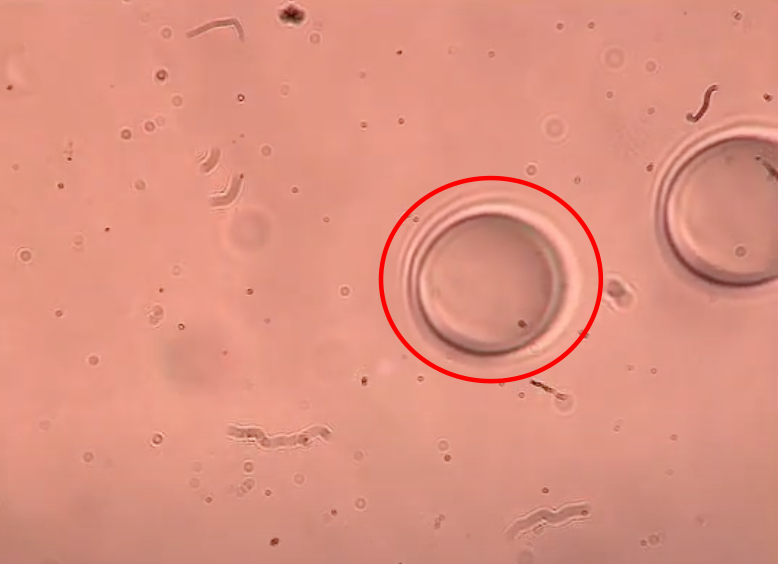
\includegraphics[width=\textwidth]{orbitando7.png}
         \caption{}
         \label{fig:five over x}
     \end{subfigure}
     \caption{Trapping of $24.82 \mu m$ $SiO_{2}$ particles. (a-f) One $SiO_2$ particle describing a circular orbit around a trapped particle (red circle). The trap was produced with the water immersion MO, and a 5x beam expander (laser power set at 96 $mW$). The stable manipulation in the z-axis was not achieved for the particles of this size.}
  \label{fig2d} 
\end{figure} %termina aquí la orbita.
%aquí empieza el 3D, jonnas video.
\begin{figure}[H]
     \centering
     \begin{subfigure}[b]{0.3\textwidth}
         \centering
         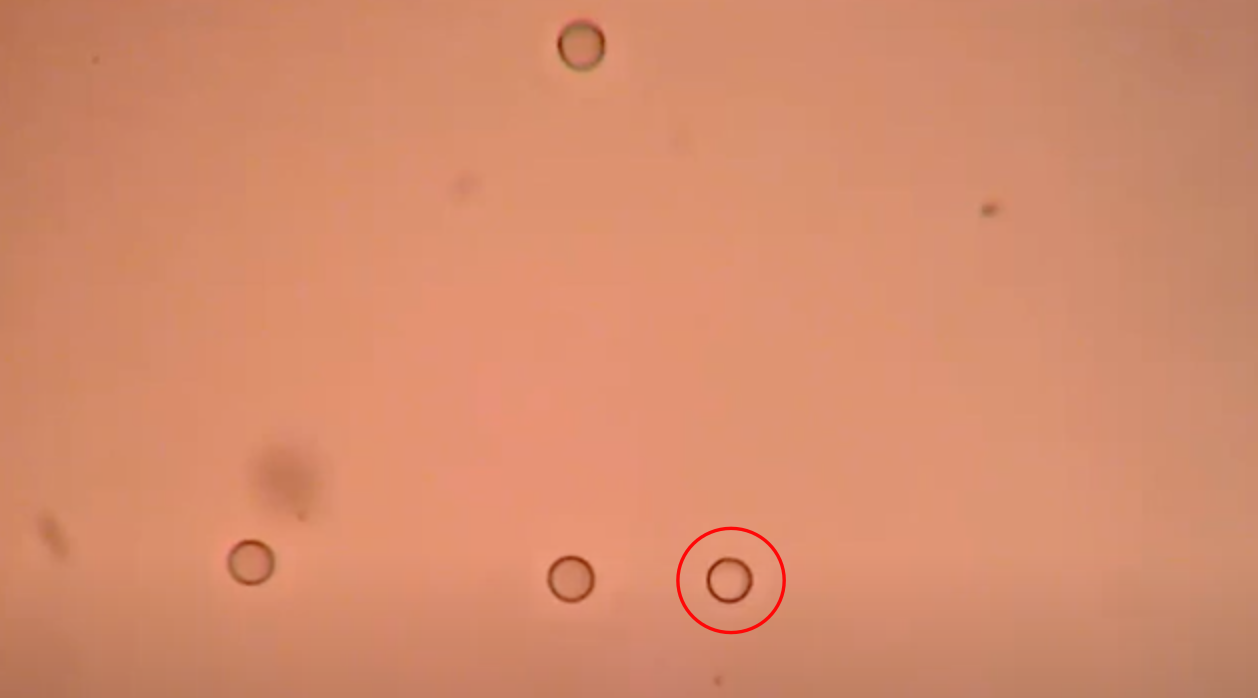
\includegraphics[width=\textwidth]{Results/jonas1redcirclenow.png}
         \caption{}
         \label{fig:y equals x}
     \end{subfigure}
     \hfill
     \begin{subfigure}[b]{0.3\textwidth}
         \centering
         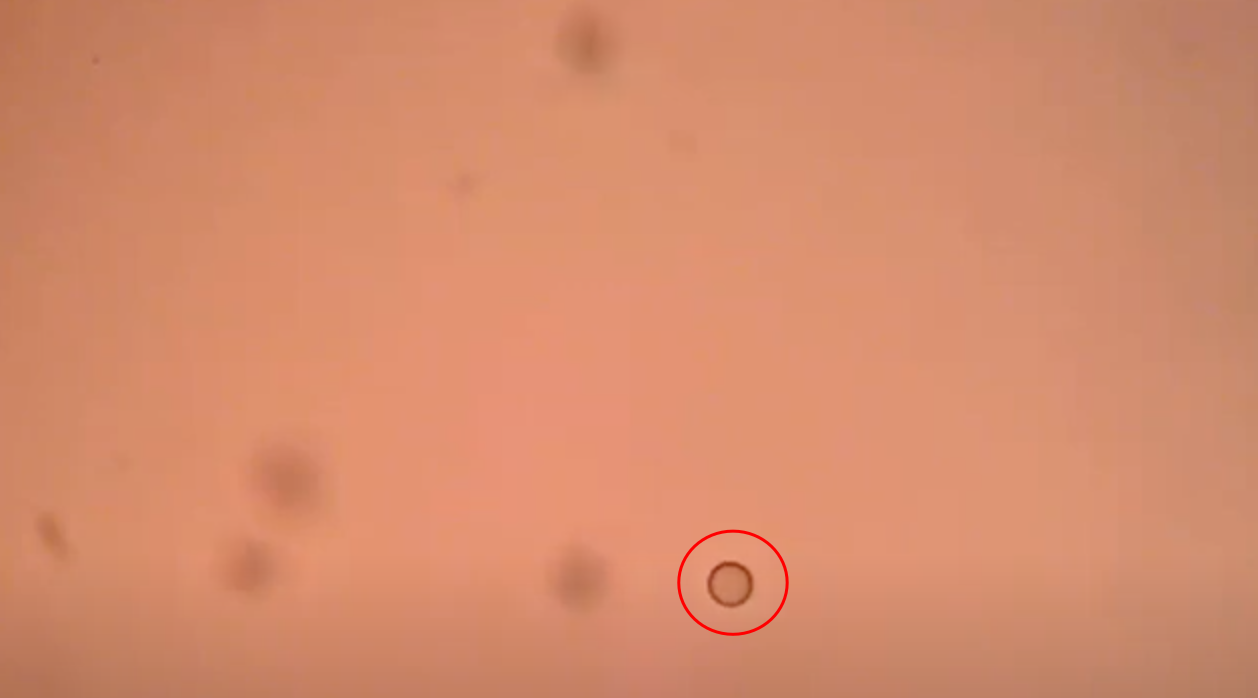
\includegraphics[width=\textwidth]{Results/jonas22222222.png}
         \caption{}
         \label{fig:three sin x}
     \end{subfigure}
     \hfill
     \begin{subfigure}[b]{0.3\textwidth}
         \centering
         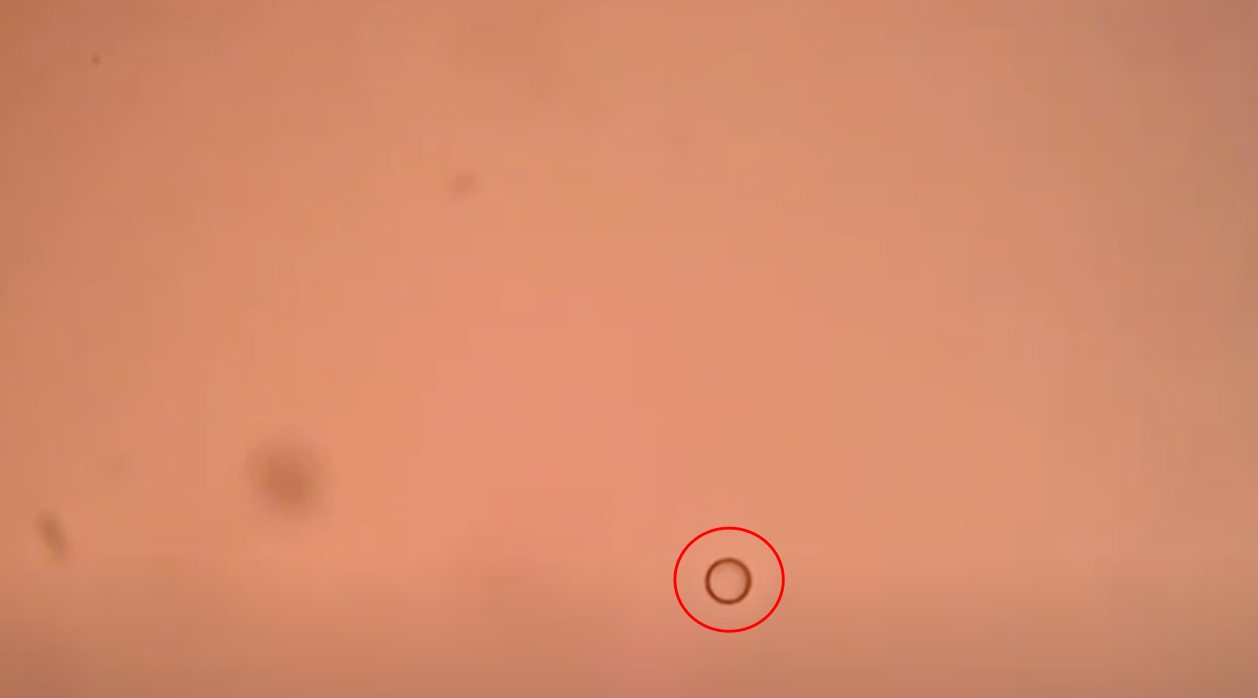
\includegraphics[width=\textwidth]{Results/jonas3circle.png}
         \caption{}
         \label{fig:five over x}
     \end{subfigure}
        \hfill
        \\\noindent \centering \begin{subfigure}[b]{0.3\textwidth}
         \centering
         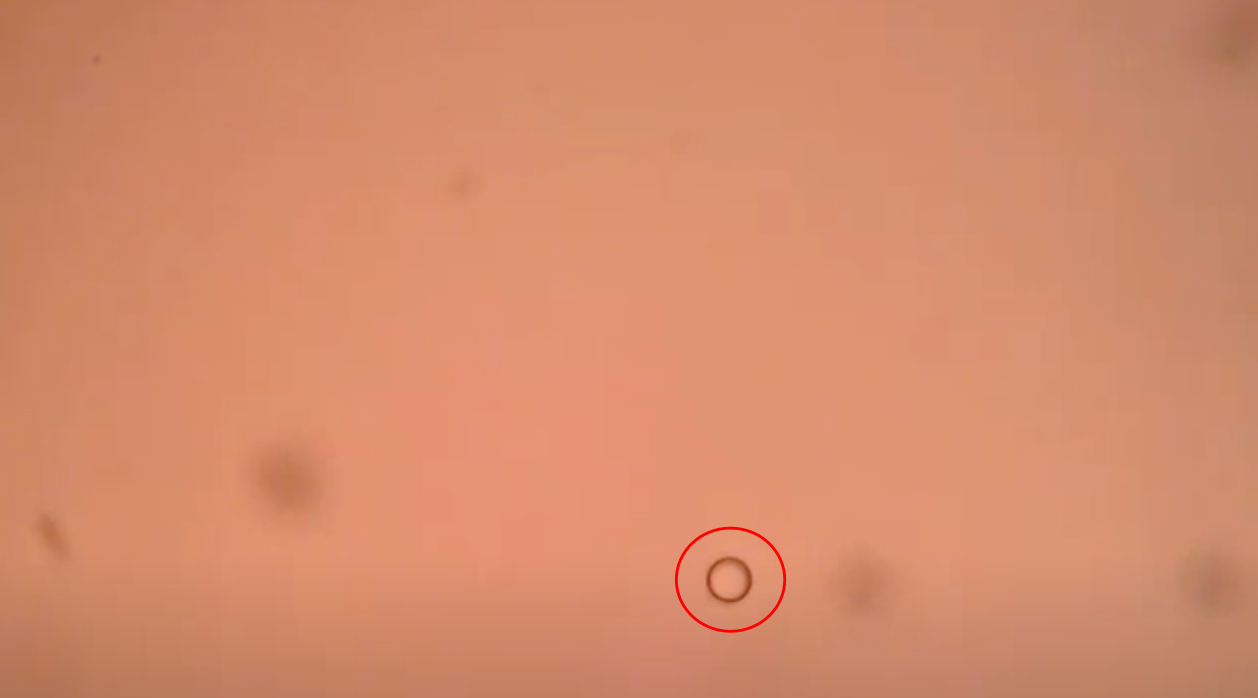
\includegraphics[width=\textwidth]{Results/jonas4.png}
         \caption{}
         \label{fig:five over x}
     \end{subfigure}
     \hfill
     \begin{subfigure}[b]{0.3\textwidth}
         \centering
         \includegraphics[width=\textwidth]{Results/jonas555.png}
         \caption{}
         \label{fig:five over x}
     \end{subfigure}
     \hfill
     \begin{subfigure}[b]{0.3\textwidth}
         \centering
         \includegraphics[width=\textwidth]{Results/circle66.png}
         \caption{}
         \label{fig:five over x}
     \end{subfigure}
     \caption{3D manipulation of $6.59 \mu m$ $SiO_2$ particles, with laser power set at 42 $mW$, and a 2x beam expander. The water immersion MO focuses the laser beam. In the image, the trapped particle is flagged with a red circle. It is moved in space while the surrounding particles remain stationary. (a) The particles are initially at the bottom of the microscope slide, with one particle already trapped using the optical tweezers. (b) The trapped particle rises due to the optical tweezers' trapping position being raised by the microscope knob. (c) The surrounding particles become less visible due to the increased distance between them and the trapped particle. (d) The surrounding particles are shifted to the right using the stage controller joystick, while the trapped particle remains in the same position. (e-f) The trapped particle is subsequently brought back to the bottom of the microscope slide using the optical tweezers. }
    \label{fig3d}
     %a)The particles are at the bottom of the microscope slide. One particle is already trapped with the optical tweezers.
\end{figure}
%termina 3D videos jonas.
%figuras de la orbita.

%\begin{figure}[H]
 %    \centering
  %   \begin{subfigure}[b]{0.3\textwidth}
   %      \centering
    %     \includegraphics[width=\textwidth]{orbitando2.png}
     %    \caption{}
      %   \label{fig:y equals x}
     %\end{subfigure}
     %\hfill
     %\begin{subfigure}[b]{0.3\textwidth}
      %   \centering
       %  \includegraphics[width=\textwidth]{orbitando3.png}
        % \caption{}
         %\label{fig:three sin x}
     %\end{subfigure}
     %\hfill
     %\begin{subfigure}[b]{0.3\textwidth}
      %   \centering
       %  \includegraphics[width=\textwidth]{orbitando4.png}
        % \caption{}
         %\label{fig:five over x}
     %\end{subfigure}
      %  \hfill
       % \\\noindent \centering \begin{subfigure}[b]{0.3\textwidth}
        % \centering
         %\includegraphics[width=\textwidth]{orbitando5.png}
         %\caption{}
         %\label{fig:five over x}
     %\end{subfigure}
     %\hfill
     %\begin{subfigure}[b]{0.3\textwidth}
      %   \centering
       %  \includegraphics[width=\textwidth]{orbitando6.png}
        % \caption{}
         %\label{fig:five over x}
     %\end{subfigure}
     %\hfill
     %\begin{subfigure}[b]{0.3\textwidth}
      %%5   \centering
         %\includegraphics[width=\textwidth]{orbitando7.png}
         %\caption{}
         %\label{fig:five over x}
     %\end{subfigure}
     %\caption{Trapping of $24.82 \mu m$ $SiO_{2}$ particles. One $SiO_2$ particle describing a circular orbit around a trapped particle (red circle). The trap was produced with the water immersion MO, and a 5x beam expander (laser power set at 96 $mW$).}
  %\label{fig7} 
%\end{figure} %termina aquí la orbita.




%The following drive contains videos for 20 $\mu m$ silica particles. These are from the second set-up with a 10x beam expander.
%\href{https://drive.google.com/drive/folders/1nEneHcXoPqPhg3C0O6HdAwIEOh7boi-6?usp=sharing}{Link 1}
%Yeast cells section
Ultimately, the manipulation of artificial $SiO_2$ particles was successfully accomplished using various beam expander configurations in conjunction with a water immersion microscope objective. The required laser power for manipulating these particles ranged from 12 to 100 $\mathrm{mW}$ across all beam expander setups tested in this study. Three-dimensional (3D) manipulation was achieved exclusively for silica particles with diameters of $6.59~\mu\mathrm{m}$ and $4.27~\mu\mathrm{m}$. In contrast, larger particles with diameters of $24.82~\mu\mathrm{m}$ and $19.98~\mu\mathrm{m}$ were only manipulated in two dimensions (2D).
\noindent After working with these beam expander configurations, the 10x system was chosen to continue the experiments with the biological entities (yeast cells and diatoms), as the magnified laser beam fully overfilled the back aperture of the microscope objectives. This configuration was preferred as the overfilling improves the trapping efficiency by allowing the outermost rays of the widened laser beam to converge at larger angles compared to those produced in the convergence of a narrower laser beam. The next step in this work was to show the capability of the optical tweezers to manipulate biological cells and examine the potential adverse effects of exposing laser light to these entities. Yeast cells were used in this regard due to their easy accessibility.
\section{Trapping and opticution of yeast cells}
After the alignment enhancement, the optical tweezers with the water immersion microscope objective were used to trap and manipulate yeast cells. To test the 3D manipulation of these bodies, they were arranged in distinctive patterns (see figure \ref{figuresyeastcells}). 
\begin{figure}[H] 
  \begin{subfigure}[b]{0.5\linewidth}
    \centering
    \includegraphics[width=0.75\linewidth,height=6.9cm]{particles2.png} 
    \caption{}    
    \label{fig7:a} 
    \vspace{4ex}
  \end{subfigure}%% 
  \begin{subfigure}[b]{0.5\linewidth}
    \centering
    \includegraphics[width=0.75\linewidth,height=6.9cm]{particles7.png} 
    \caption{}
    \label{fig7:b} 
    \vspace{4ex}
  \end{subfigure} 
  \begin{subfigure}[b]{0.5\linewidth}
    \centering
    \includegraphics[width=0.75\linewidth]{particlesnow.png} 
    \caption{}
    \label{fig7:c} 
  \end{subfigure}%%
  \begin{subfigure}[b]{0.5\linewidth}
    \centering
    \includegraphics[width=0.75\linewidth]{Particles3.png} 
    \caption{}
    \label{fig7:d} 
  \end{subfigure} 
  \caption{Trapping of yeast cells with the water immersion MO, laser power set at 14 $mW$ with 10x beam expander. (a-d) The optical tweezers arranged the trapped yeast cells on the coverslide's surface, creating distinctive patterns and figures.}
  \label{figuresyeastcells}
\end{figure}
\noindent The photodamage of the yeast cells due to the optical tweezers (opticution) was observed when increasing considerably the laser power. The following figure shows the opticution of a trapped yeast cell at 695 $mW$. The cell exploded after roughly one second of being subjected to the laser beam. Below this laser power, specifically at $645 mW$,
and $595 mW$, the explosion of the yeast cell was also observed but took a longer time being subjected to the laser beam. 
%%%
%%Opticution
%%%
%%%
\begin{figure}[H]
     \centering
     \begin{subfigure}[b]{0.49\textwidth}
         \centering
         \includegraphics[width=0.80\textwidth]{Imagenes teoria/opticution0_edited.jpeg}
         \caption{Trapped yeast cell with 14 $mW$}
         \label{fig:y equals x}
     \end{subfigure}
     \hfill
     \begin{subfigure}[b]{0.49\textwidth}
         \centering
         \includegraphics[width=0.80\textwidth]{Imagenes teoria/opticution1_edited.jpeg}
         \caption{Opticuted yeast cell with 695 $mW$}
         \label{fig:three sin x}
     \end{subfigure}
     
     \caption{Opticution (dead by light) of a yeast cell with a 10x beam expander, and the water immersion microscope objective.}
     \label{opticution}
     \hfill
\end{figure}
\noindent
\section{Trapping of Diatoms} %%%A %%
With the previous results, the trapping experiments for diatoms, the main focus of this work, began. Given the nature of the frustules, which are made of silica similar to the previously trapped particles, their optical manipulation was expected beforehand. %optical tweezers previously, so their manipulation with these devices was expected beforehand. %single cell study ponerlo al final. %de trapping diatoms

Indeed, the diatom species' manipulation was achieved with both the water and oil immersion microscope objectives. The only exceptions were the \textit{Marine pennate} and the \textit{Navicula Sp.12} species, which were only manipulated with the water immersion microscope objective. The following images show the trapping and manipulation with the optical tweezers of the species of diatoms based on their symmetry. 

\subsection{Manipulation and trapping of pennate Diatoms}
For these experiments, the optical tweezers employed the 10x beam expander, only the \textit{Marine pennate} species was manipulated with a 2x configuration since it was part of a previous batch of algae samples and was off during the experiments with the other species. The first manipulated algae with both microscope objectives was the \textit{Nitzchia Sp.1} (see figures \ref{WIMOFIRST1} and \ref{OIMOFIRST2}) %The species trapped with the 10x configuration had different symmetries (pennate and centric algae) and were trapped with different laser powers under the 100 $mW$ bound.
%First water algae.
\begin{figure}[H] 
  \begin{subfigure}[b]{0.5\linewidth}
    \centering
    \includegraphics[scale=0.3]{ResultadosAlgea1/11.png} 
    \caption{}
    \label{fig7:a} 
    \vspace{4ex}
  \end{subfigure}%% 
  \begin{subfigure}[b]{0.5\linewidth}
    \centering
    \includegraphics[scale=0.3]{ResultadosAlgea1/levantando.png} 
    \caption{}
    \label{fig7:b} 
    \vspace{4ex}
  \end{subfigure} 
  \begin{subfigure}[b]{0.5\linewidth}
    \centering
    \includegraphics[scale=0.3]{ResultadosAlgea1/3.png} 
    \caption{}
    \label{fig7:c} 
  \end{subfigure}%%
  \begin{subfigure}[b]{0.5\linewidth}
    \centering
    \includegraphics[scale=0.3]{ResultadosAlgea1/1.png} 
    \caption{}
    \label{fig7:d} 
  \end{subfigure} 
  \caption{Manipulation of \textit{Nitzschia Sp.1} (pennate) with the water immersion MO, and a 10x beam expander. The laser power was set at 25 $mW$. (a-d) Frames from the recorded video when subjecting the diatom to the laser beam: (a) First, the particle lies on the microscope slide surface with the laser off. (b-c) When the laser is turned on, the diatom starts transitioning toward its trapped position within the optical tweezers (subfigure (d)) due to the gradient force. The figures are ordered chronologically, and the diatom subjected to the laser beam is marked with a black circle.}
  \label{WIMOFIRST1} 
\end{figure}
%%%%
%First algae oil 
%%%
%%%
\begin{figure}[H] 
  \begin{subfigure}[b]{0.5\linewidth}
    \centering
    \includegraphics[scale=0.3]{Results/Oilnitzchia/firstoil1.png} 
    \caption{}
    \label{fig7:a} 
    \vspace{4ex}
  \end{subfigure}%% 
  \begin{subfigure}[b]{0.5\linewidth}
    \centering
    \includegraphics[scale=0.3]{Results/Oilnitzchia/oil2first.png} 
    \caption{}
    \label{fig7:b} 
    \vspace{4ex}
  \end{subfigure} 
  \begin{subfigure}[b]{0.5\linewidth}
    \centering
    \includegraphics[scale=0.3]{Results/Oilnitzchia/oilfirst3.png} 
    \caption{}
    \label{fig7:c} 
  \end{subfigure}%%
  \begin{subfigure}[b]{0.5\linewidth}
    \centering
    \includegraphics[scale=0.3]{Results/Oilnitzchia/forthoilnitzchia.png} 
    \caption{}
    \label{fig7:d} 
  \end{subfigure} 
  \caption{Manipulation of \textit{Nitzschia Sp.1} (pennate) with the oil immersion MO, and a 10x beam expander. The laser power was set at 47 $mW$. (a-d) Frames from the recorded video when subjecting the diatom to the laser beam: (a) First, the particle lies on the microscope slide surface with the laser off. (b-c) The diatom starts rotating when the laser is turned on to align with the z-axis (subfigure (d)) due to the gradient force.  The figures are ordered chronologically, and the diatom subjected to the laser beam is marked with a black oval.}
  \label{OIMOFIRST2} 
\end{figure}
%%
%%
%%second algea image.
%%
%%
\noindent The second algae with bilateral symmetry trapped with the microscope objectives was the \textit{Phaeodactylum tricornutum} (see figures \ref{WISECOND1} and \ref{OISECOND2}).
\begin{figure}[H] 
  \begin{subfigure}[b]{0.5\linewidth}
    \centering
    \includegraphics[scale=0.20]{Results/Resultadosalgea2/firstwatter secondalgea.png} 
    \caption{}
    \label{fig7:a} 
    \vspace{4ex}
  \end{subfigure}%% 
  \begin{subfigure}[b]{0.5\linewidth}
    \centering
    \includegraphics[scale=0.20]{Results/Resultadosalgea2/secondalgea2water.png} 
    \caption{}
    \label{fig7:b} 
    \vspace{4ex}
  \end{subfigure} 
  \begin{subfigure}[b]{0.5\linewidth}
    \centering
    \includegraphics[scale=0.2]{Results/Resultadosalgea2/secondalgeawater3.png} 
    \caption{}
    \label{fig7:c} 
  \end{subfigure}%%
  \begin{subfigure}[b]{0.5\linewidth}
    \centering
    \includegraphics[scale=0.2]{Results/Resultadosalgea2/secondalgeawater4.png} 
    \caption{}
    \label{fig7:d} 
  \end{subfigure} 
  \caption{Trapping of \textit{Phaeodactylum tricornutum} (pennate) with the water immersion MO, and a 10x beam expander. The laser power was set at 19 $mW$. (a-d) Frames from the recorded video when subjecting the diatom to the laser beam: (a) First, the particle lies on the microscope slide surface with the laser off. (b-c) When the laser is turned on, the diatom starts transitioning toward its trapped position within the optical tweezers (subfigure (d)) due to the gradient force. The figures are ordered chronologically, and the trapped diatom is marked with a black oval.
}
  \label{WISECOND1} 
\end{figure}
%%
%%
%%Oil second algae
%%
%%
\begin{figure}[H]
     \centering
     \begin{subfigure}[b]{0.49\textwidth}
         \centering
         \includegraphics[width=0.6\textwidth]{Results/Resultadosalgea2/oil1.png}
         \caption{}
         \label{fig:y equals x}
     \end{subfigure}
     \hfill
     \begin{subfigure}[b]{0.49\textwidth}
         \centering
         \includegraphics[width=0.60\textwidth]{Results/Resultadosalgea2/oilt2.png}
         \caption{}
         \label{fig:three sin x}
     \end{subfigure}
     \caption{Trapping of \textit{Phaeodactylum tricornutum} (pennate) with the oil immersion MO, and a 10x beam expander. The laser power was set at 27 $mW$. (a) The diatom lies on the surface of the microscope slide when the laser is off. (b) The laser is turned on, and the diatom reaches its trapped position within the optical tweezers due to the gradient force. In the figures, the trapped diatom is
marked with a black oval.}
\label{OISECOND2}
     \hfill
    %%
\end{figure}
%%Forth algae historically, third 
%%%
%%%
\noindent The following images show the trapping of the \textit{Navicula Sp.12} and the \textit{Marine pennate} species with the water immersion microscope objective (see figure \ref{WITHIRD1},\ref{WIFORTH1}).
\begin{figure}[H]
     \centering
     \begin{subfigure}[b]{0.3\textwidth}
         \centering
         \includegraphics[width=\textwidth]{Results/Resultsforthalgae/falgae1_#image2327.png}
         \caption{}
         \label{fig:y equals x}
     \end{subfigure}
     \hfill
     \begin{subfigure}[b]{0.3\textwidth}
         \centering
         \includegraphics[width=\textwidth]{Results/Resultsforthalgae/falgae2.png}
         \caption{}
         \label{fig:three sin x}
     \end{subfigure}
     \hfill
     \begin{subfigure}[b]{0.3\textwidth}
         \centering
         \includegraphics[width=\textwidth]{Results/Resultsforthalgae/falgae3.png}
         \caption{}
         \label{fig:five over x}
     \end{subfigure}
       
     \caption{Trapping of \textit{Navicula Sp.12} with the water immersion MO (pennate), and a 10x beam expander. The laser power was set at 31 $mW$. (a-c) Chronologically ordered frames from the recorded video of the trapping of the \textit{Navicula Sp.12} diatom. (a) The diatom starts lying on the surface of the microscope slide when the laser is off. (b-c) When the laser is turned on, the diatom transitions toward its trapped position within the optical tweezers due to the gradient force. In the figures, the trapped diatom is marked with a black circle.}
\label{WITHIRD1}
     
\end{figure}
%%%
%%%FIfth algae
\begin{figure}[H]
     \centering
     \begin{subfigure}[b]{0.3\textwidth}
         \centering
         \includegraphics[width=\textwidth]{Results/Fifth/pennate1water.png}
         \caption{}
         \label{fig:y equals x}
     \end{subfigure}
     \hfill
     \begin{subfigure}[b]{0.3\textwidth}
         \centering
         \includegraphics[width=\textwidth]{Results/Fifth/pennatewater2.png}
         \caption{}
         \label{fig:three sin x}
     \end{subfigure}
     \hfill
     \begin{subfigure}[b]{0.3\textwidth}
         \centering
         \includegraphics[width=\textwidth]{Results/Fifth/pennate3water.png}
         \caption{}
         \label{fig:five over x}
     \end{subfigure}
       
     \caption{Trapping of \textit{Marine pennate} (pennate) with the oil immersion MO, and a 2x beam expander. The laser power was set at 232 $mW$. (a-c) Chronologically ordered frames from the recorded video of the trapping of the mentioned pennate diatom. (a) The diatom starts lying on the surface of the microscope slide when the laser is off. (b-c) When the laser is turned on, the diatom transitions toward its trapped position within the optical tweezers due to the gradient force. In the figures, the trapped diatom is marked with a red oval.}
\label{WIFORTH1}
     
\end{figure}
\noindent The shape of the particles plays an important role in the trapping performance of the optical tweezers. Pennate diatoms, characterized by their bilateral symmetry, tend to rotate aligning their symmetry axis to match the symmetry axis of the focused laser beam.  This behavior was observed during the experiments as can be seen in the figures. On the other hand, the trapping of the centric diatom \textit{Thalassiosira pseudonana} was also achieved with both microscope objectives.
\subsection{Trapping of the centric Diatom \textit{Thalassiosira pseudonana}}
The following images show the trapping of the \textit{Thalassiosira pseudonana} with the water and the oil immersion microscope objectives. In the figures, the trapped particle is held by the optical tweezers, while the surrounding ones change their position following the action of the microscope stage. 
%%%
%%%
%%%Pseudonana water
%%%
%%%
\begin{figure}[H] 
  \begin{subfigure}[b]{0.5\linewidth}
    \centering
    \includegraphics[scale=0.28]{Results/Pseudonana water/wpseudona1.png} 
    \caption{}
    \label{fig7:a} 
    \vspace{4ex}
  \end{subfigure}%% 
  \begin{subfigure}[b]{0.5\linewidth}
    \centering
    \includegraphics[scale=0.28]{Results/Pseudonana water/wpseudonana2.png} 
    \caption{}
    \label{fig7:b} 
    \vspace{4ex}
  \end{subfigure} 
  \begin{subfigure}[b]{0.5\linewidth}
    \centering
    \includegraphics[scale=0.28]{Results/Pseudonana water/wpseudonana3.png} 
    \caption{}
    \label{fig7:c} 
  \end{subfigure}%%
  \begin{subfigure}[b]{0.5\linewidth}
    \centering
    \includegraphics[scale=0.28]{Results/Pseudonana water/wpseudonana4.png} 
    \caption{}
    \label{fig7:d} 
  \end{subfigure} 
  \caption{Trapping of \textit{Thalassiosira pseudonana}(centric) with the water immersion MO, and a 10x beam expander. The laser power was set at 11 $mW$. (a-d) Frames from
the recorded video when subjecting the diatom to the laser beam: The trapped particle remains still due to the action of the gradient force, while the surrounding particles changed their relative position. In the figures, the trapped diatom is
marked with a black circle.}
  \label{} 
\end{figure}
%%
%%
%%Oil Pseudonana
%%
%%
\begin{figure}[H] 
  \begin{subfigure}[b]{0.5\linewidth}
    \centering
    \includegraphics[scale=0.3]{Results/ResultsOilpseudonana/op1.png} 
    \caption{}
    \label{fig7:a} 
    \vspace{4ex}
  \end{subfigure}%% 
  \begin{subfigure}[b]{0.5\linewidth}
    \centering
    \includegraphics[scale=0.3]{Results/ResultsOilpseudonana/op2.png} 
    \caption{}
    \label{fig7:b} 
    \vspace{4ex}
  \end{subfigure} 
  \begin{subfigure}[b]{0.5\linewidth}
    \centering
    \includegraphics[scale=0.3]{Results/ResultsOilpseudonana/op3.png} 
    \caption{}
    \label{fig7:c} 
  \end{subfigure}%%
  \begin{subfigure}[b]{0.5\linewidth}
    \centering
    \includegraphics[scale=0.3]{Results/ResultsOilpseudonana/op4.png} 
    \caption{}
    \label{fig7:d} 
  \end{subfigure} 
  \caption{Trapping of \textit{Thalassiosira pseudonana} (centric) with the oil immersion MO, and a 10x beam expander. The laser power was set at 91 $mW$. (a-d) Frames from
the recorded video when subjecting the diatom to the laser beam: The trapped diatom remains still due to the action of the gradient force, while the surrounding ones changed their relative position. In the figures, the trapped diatom is
marked with a black circle. }
  \label{} 
\end{figure}

%It is important to notice that depending on the symmetry of the Diatom, the trapping is perceived differently in the figures. The centric Diatom textit{Thalassiosira Pseudonana 132} was held by the optical tweezers while the surrounding particles were moved (to show the trapping). On the other hand, when the penate Diatoms were trapped, their symmetrical axis rotated to match the optical axis of the trap.
\noindent This section demonstrated the manipulation of diatoms with different symmetries using optical tweezers. This aspect is important in the advancement toward the achievement of the long-term goal of this project since it sets the stage for further exploration in single-cell research for Diatoms. In the same context, the subsequent logical step was to incorporate microfluidic devices into this study.
% usage of optical tweezers opens the way to produce further single-celled studies due to their ability to control the 3D position of the trapped particle. 
\section{Trapping in microfluidic channel}
%Agregar force quantitative, and thje similar size of the particles and the only diference is the pores. 
The trapping of Diatoms flowing in the microfluidic channels was achieved for different flow velocities and species. Specifically, the \textit{Thalassiosira pseudonana}, and the \textit{Phaeodactylum tricornutum} were trapped in a stable manner while flowing in the microfluidic channels. Furthermore, the 6.59$\mu m$ synthetic $SiO_2$ particles were stably trapped in the microfluidic channels. A size comparison between these spherical $SiO_2$ particles and the centric \textit{Thalassiosira pseudonana} species was performed using camera images, in which they were found to be roughly the same size. Since the diatom frustule is made of the same material as the artificial particle, the only difference comes from the pores encrusted on the first, which is also accredited for their distinctive optical properties. So, a first approximation towards the characterization of the photonic properties of diatoms was to compare the performance of the optical tweezers for this species against the $SiO_2$ particles. 

\noindent
To quantify this performance, the threshold flow velocities for the two particles were measured at different laser powers. The threshold flow velocity refers to the velocity required to release the trapped particle from the optical tweezers at a given laser power. In this study, for each laser power, the threshold flow velocity was measured ten times to determine the average value, which we will refer to as the average threshold flow velocity (ATFV). The operating laser powers used for these measurements were \text{141, 130, 120, 110, 90, 80, 70, 60, 50, and 40\,mW} for \textit{Thalassiosira pseudonana}, and \text{120, 110, 100, 90, and 80\,mW} for the artificial silica particle.
The results of these measurements are shown in the following figure (see figure \ref{graficasmicrofluidics})
\begin{figure}[H]
     \centering
     \begin{subfigure}[b]{0.49\textwidth}
         \centering
         \includegraphics[width=0.95\textwidth]{Newplots_microfluidics_results/Silica_particles.png}
         %surpass the gradient force.
         \caption{Optical tweezers performance for the spherical 6.59 $\mu m$ $SiO_2$ particles.}
         \label{fig:y equals x}
     \end{subfigure}
     \hfill
     \begin{subfigure}[b]{0.49\textwidth}
         \centering
         \includegraphics[width=0.95\textwidth]{Newplots_microfluidics_results/Thala.png}
         \caption{Optical tweezers performance for the \textit{Thalassiosira pseudonana} diatom.}
         \label{fig:three sin x}
     \end{subfigure}
     \caption{Average threshold flow velocity (ATFV) to surpass the gradient force of the optical tweezers for (a) spherical artificial silica particles, and (b) \textit{Thalassiosira pseudonana} diatom. The vertical axis represents the average threshold flow velocity with standard deviation $(\sigma)$ for the different laser powers at the horizontal axis.}
     \hfill
    \label{graficasmicrofluidics} 
\end{figure}






%The threshold flow velocities to remove the $SiO_2$ particles from the laser trap were measured for the centric Diatom Thalassiosira Pseudonana 132, and the 6.59$\mu m$ artificial particles for different laser powers.  These measurements were used to compare the optical tweezers' performance for these two particles (see figure \ref{graficasmicrofluidics}).

%These two particles were chosen since, they have the same symmetry, are made of the same material, and have roughly the same size. The only difference between them is the intrinsic patterns of pores in the algae body (frustule), which are the ones producing their remarkable optical properties.\\
\noindent From the graphics, we can observe a different performance of the optical tweezers for both silica bodies. The velocity threshold decreases when the laser power decreases for both of them. However, the decaying is more pronounced for the algae, which also had a lower velocity threshold for a higher laser power than the artificial spherical particle, indicating lower trapping performance for the diatom. It is important to note that incorporating microfluidic devices provides a quantifiable way to characterize the trapping performance for particles.
Specifically, measuring the average threshold flow velocity is valuable because it serves as an indirect measure of the force exerted on the trapped particle by the flowing liquid, which counteracts the transversal force generated by the optical tweezers (i.e., the gradient force). Considering the linear velocity of the fluid, and assuming both silica bodies are perfect spheres with a radius of \( R = 6.59 \, \mu m \), and that the viscosity of seawater is \( 8.8 \times 10^{-4} \, N \cdot s/m^2 \), Stokes' law provides an approximation for the drag forces counteracting the gradient forces in our experiment.  These forces are illustrated in the following figure (see figure \ref{forces_microfluidcs})
%Forces plots
\begin{figure}[H]
     \centering
     \begin{subfigure}[b]{0.49\textwidth}
         \centering         \includegraphics[width=0.95\textwidth]{Newplots_microfluidics_results/Force_silica_particle.png}
         %surpass the gradient force.
         \caption{Optical tweezers performance for the spherical 6.59 $\mu m$ $SiO_2$ particles.}
         \label{fig:yx}
     \end{subfigure}
     \hfill
     \begin{subfigure}[b]{0.49\textwidth}
         \centering
         \includegraphics[width=0.95\textwidth]{Newplots_microfluidics_results/Force_Thalassiosira.png}
         \caption{Optical tweezers performance for the \textit{Thalassiosira pseudonana} diatom.}
         \label{figx}
     \end{subfigure}
     \caption{Drag force necessary to surpass the gradient force of the optical tweezers for (a) spherical artificial silica particles, and (b) \textit{Thalassiosira pseudonana} diatom. The vertical axis represents the Stokes' force for the different laser powers at the horizontal axis.}
     \hfill
    \label{forces_microfluidcs} 
\end{figure}
Due to the fact that the Stokes' force and the average threshold flow velocity are constant factors away, in figure \ref{forces_microfluidcs}, we can observe the same pattern for the forces as in figure \ref{graficasmicrofluidics} for the velocities, with a change in the magnitude scale and units natural of the calculation of forces and flow rates. 
Since we are measuring the Stokes' force at the breaking point, we can equate it to the gradient force arising from the optical tweezers, which characterizes the optical tweezers setup. It is important to note a difference factor of 10 between the theoretical approximations presented earlier and the experimental results, being the experimental force for the particles bigger than the theoretical calculation. Overall, we observe a difference in the performance of the optical tweezers for both silica bodies, indicating a physical distinction between them or even suggesting a difference in the light-matter interaction occurring when subjected to the laser beam. In this sense, this experiment serves as a first approximation to shed light on the effects of the frustule pores on the performance of the optical tweezers.

    
\chapter{Conclusions}  
Two of the most emblematic additions brought by optical tweezers to the research of microscopic things were the contactless 3D manipulation of dielectric particles and the application of these devices to investigate biological entities. Such applications to biological sciences merited Artur Ashkin a Nobel prize in physics. \newline 
In this line, this work can be split into two main ideas: manipulating particles of different nature and a first approximation to applying optical tweezers to perform research with diatoms.
The first part of this work demonstrated the implementation and enhancement of optical tweezers to manipulate different microscopic bodies. In this part, mainly particles of spherical symmetry were studied. Different beam expander configurations were tested by running experiments with the particles to determine the one with the best performance. Specifically, artificial silica particles of spherical shapes with diameters of \(4.25 \, \mu m\) and \(4.27 \, \mu m\) were stably trapped in three-dimensional space (3D manipulation). In contrast, larger particles with diameters of \(24.82 \, \mu m\) and \(19.98 \, \mu m\) were only manipulated in the horizontal plane (2D manipulation), likely due to their relatively larger size. Additionally, this work demonstrates the 3D manipulation of yeast cells, enabling the formation of patterns and figures on the surface of the microscope slide. Cell death by light ("opticution") of the yeast cells is also reported for different laser operating powers.
%We find the yeast cells and the silica particles of different sizes ($4.27 \mu m$, $6.59 \mu m$, and $24.82 \mu m$) between the spherical particles trapped in this work. 
The trapping of the particles in the first part was expected due to their widespread use in optical tweezers experiments. %Historically, the first report of silica particles being optically trapped was done by Ashkin himself in his seminal paper on the observation of the single-beam gradient force optical trap (currently named optical tweezers) for dielectric particles. 

\newline 
The successful manipulation and opticution of yeast cells served as a preamble to the second part of this work, which demonstrates the application of optical tweezers to study biological entities, specifically diatoms. %Priorly, the achieved manipulation and opticution of yeast cells served as a preamble to transition to the study of diatoms.
The manipulation of different diatom species was achieved in this part, such as the \textit{Nitzchia Sp.1}, \textit{Phaeodactylum tricornutum}, \textit{Navicula Sp. 12}, \textit{Marine pennate}, and the \textit{Thalassiosira pseudonana} species. Diatoms with bilateral symmetry tended to rotate, aligning their symmetry axis with the vertical axis.
Additionally, microfluidic devices were integrated to enable quantifiable analysis of the optical tweezers' trapping performance. Specifically, these devices were utilized to measure the average fluid velocity required to free the trapped \textit{Thalassiosira pseudonana} and the $6.59~\mu\text{m}$ particles from the optical tweezers at a given laser power. This velocity threshold serves as an indicator of the optical tweezers' performance. Furthermore, the threshold velocity measurements were extended to compute the Stokes' force, which, at the breaking point, equates to the gradient force. Thus, the incorporation of microfluidic devices allowed for a characterization of the optical tweezers used in the experiments. The experimentally measured gradient force for the $6.59~\mu\text{m}$ particles was an order of magnitude larger than the theoretical value calculated in the theoretical background chapter. This discrepancy might partly be attributed to the microfluidic system's sensitivity to minor pressure changes or to the calibration of the syringe pump. In addition, the computation of the gradient force through the Stokes' force, though straightforward, presents other possible causes for the aforementioned discrepancy between the theoretical and experimental forces. In particular, the viscosity of the seawater used to compute the Stokes' force can vary due to temperature changes, and in an actual liquid flow (even at low Reynolds numbers) the velocity profile across the transverse section is not uniform. This velocity profile is parabolic in shape, with the outermost streamlines (at the bottom and top of the microfluidic channel) exhibiting lower velocities. These velocities decrease further and approach zero near the channel walls. In this work, trapping was performed close to the surface of the microfluidic channels and coverslip, as these regions were easily identified by marking the top surface with a marker pen beforehand. This suggests that the streamlines flowing around the trapped particle had a lower velocity magnitude, resulting in a weaker force than the one computed directly using the Stokes' formula.
Additionally, it was found that the optical tweezers constructed in this work had different trapping performance for the centric diatom \textit{Thalassiosira pseudonana} and the artificial $SiO_2$ particle.
This difference might be interpreted as a first approximation to characterizing the optical properties of the frustule since the structural difference between the \textit{Thalassiosira pseudonana} species and the artificial particles lies on the pores encrusted in the frustule surface, which could influence the optical trapping behavior. %The measurement of the threshold velocity was extended to the computation of the Stoke's force which in the breaking point equates the gradient force. In this sense, integrating the microfluidic devices provided a characterization of the optical tweezers employed during the experiments.


%aqui va


%Additionally, it was observed that the optical tweezers constructed in this study exhibited varying performance efficiencies when trapping the centric diatom \textit{Thalassiosira pseudonana} compared to the artificial $\text{SiO}_2$ particles. This difference can be interpreted as a preliminary step toward characterizing the optical properties of the diatom frustule. The structural distinction between \textit{Thalassiosira pseudonana} and the artificial particles lies in the pores embedded in the frustule surface, which likely influence the optical trapping behavior.

%By extending the threshold velocity measurements to the computation of the Stokes force, the study provided a more robust characterization of the optical tweezers' performance. Overall, the integration of microfluidic devices proved instrumental in elucidating the operational dynamics of the optical tweezers during the experiments.
%aqui vanki



%This can be done in a future work by taking into account the viscosity and density of the liquid media.\\It is worth noting that the optical tweezers allow the elaboration of a single-cell study of diatoms to continue this work. 

Regarding future advances based on this work, it is worth noting that optical tweezers enable detailed single-cell studies of diatoms, providing a foundation for further research. From the theoretical perspective of this work, the forces involved in trapping such particles can be more precisely described analytically using the generalized Lorenz-Mie theory. %In this regard, this work can be extended by characterizing these forces for particles of different sizes and shapes, even considering in the calculations the frustule structure for the diatoms. 
As of the experimental aspect of this work, a comparison for the trapping of different wavelengths can be pursued, and since the trapping of these particles was achieved for different magnification systems, a comparison can also be conducted for this parameter. This future study could be further complemented by implementing microfluidic channels to change the medium in which the diatoms are suspended while trapped. This would enable direct observation of the effects of such changes on their reproduction process. However, this approach presents both an opportunity and a potential challenge, as it requires addressing the effects of radiation on the organic material within the frustule. Laser light can cause photodamage to the cell as showcased with the opticution of the yeast cells, potentially inhibiting the reproductive capabilities of the diatom specie. This issue could be solved by changing the wavelength used to produce the trap to one in the infrared range. Therefore, a deeper study of the photonic properties of the frustule should be done. This would add to the investigations on the detrimental ultraviolet light protection exhibited by the frustule, which has been reported previously. In this line, a spectroscopy study could shine light onto the action of the frustules to focus deterrent radiation outside the organic components of the cell. These investigations would help address some of the questions posed at the beginning of this work, which motivated the use of optical tweezers and microfluidic channels for comprehensive single-cell studies of diatoms.

%Regarding future advances based on this work, it is worth noting that optical tweezers enable detailed single-cell studies of diatoms, providing a foundation for further research. From a theoretical perspective, the forces involved in trapping such particles can be fully described analytically using the generalized Lorenz-Mie theory. In this regard, this work can be extended by characterizing these forces for particles of different sizes and shapes. Additionally, a comparison of trapping efficiency for different wavelengths could be pursued. Since the trapping of these particles was achieved using different magnification systems, a comparative analysis of this parameter could also be conducted.
 %This issue could be mitigated by using a wavelength in the infrared range for trapping, which is less likely to cause damage.

%To achieve this, a deeper study of the photonic properties of the frustule is necessary, which would contribute to the characterization of these properties. Furthermore, a spectroscopy study could provide insights into how the frustule focuses or deflects radiation away from the organic components of the cell. Such investigations would help address some of the key questions that motivated the use of optical tweezers and microfluidic channels for comprehensive single-cell studies of diatoms in this study.




%Regarding future advances based on this work, it is worth noting that optical tweezers enable detailed single-cell studies of diatoms, providing a strong foundation for further research.  

%From a theoretical perspective, the forces involved in trapping such particles can be fully described analytically using generalized Lorenz-Mie theory. This work can be extended by characterizing these forces for particles of different sizes and shapes. Additionally, a comparison of trapping efficiency for different wavelengths could be pursued. Since trapping was achieved using various magnification systems, a comparative analysis of this parameter could also be conducted.  

%Future studies could be further enhanced by implementing microfluidic channels to change the medium in which the diatoms are suspended while trapped. This would allow direct observation of the effects of such changes on their reproduction process. However, this approach presents both an opportunity and a potential challenge, as the effects of laser radiation on the organic material within the frustule must be carefully considered. Laser light can cause photodamage to the cell, potentially inhibiting its reproductive capabilities. This issue could be mitigated by using a wavelength in the infrared range for trapping.  

%To support these advancements, a deeper study of the photonic properties of the frustule is necessary, which would contribute to the overall characterization of these structures. Furthermore, spectroscopic studies could provide insights into how the frustules focus or deflect harmful radiation away from the organic components of the cell.  

%Oil immersion, 



%For the first set-up: \newline To optimize the optical tweezers, it is clear the need of a dichroic mirror
%for 532 nm and a different camera. Since, in our experiments bigger silica
%particles are to be studied, the power of the laser output should not be
%reduced by a factor of 1
\\\\\noindent
%For the second set-up:\\ The particles where trapped and manipulated in a 2D trap. The backscattered radiation pattern was better. However, I could no move the particle in the z-direction. This was due to misalignments in the z axis. 
\appendix
\chapter{Laser light}
\section{Laser Light}
Laser light is a form of electromagnetic radiation. 
The word "Laser" is an acronym for "Light Amplification
by Stimulated Emission of Radiation" \cite{svelto2010principles}. It refers to the process by which light is produced. This process is usually not observable in nature \cite{nilsson2020development} and endows the laser device properties that differ it from other ordinary light sources \cite{svelto2010principles}.


\subsection{Properties of laser light.}
\begin{itemize}
    \item Monochromaticity.
    Laser light possesses a narrow bandwidth \cite{svelto2010principles}. In contrast, white light is a combination of different wavelengths. 
    
    \item Directionality. A laser beam possesses small divergence angles \cite{svelto2010principles}.
    \item Coherence. The laser beam is coherent (spatially and temporally) \cite{svelto2010principles}.
    \item Brightness. Even a low-power (few milliwatts) operating laser possesses a brightness of
several orders of magnitude greater than that of the brightest conventional sources \cite{svelto2010principles}.
\item Diverse beam profiles. The term "beam profile" refers to the spatial arrangement of light intensity across the beam's cross-sectional area. One notable characteristic of laser beams is their capability to manifest in various beam profiles. The most common and well-known is the Gaussian or bell-shaped beam profile. %Laser light can assume distinct spatial intensity distributions, thereby offering a range of beam profiles. % if the Gaussian beam profile section isnt needed then I could write the following and jump to the optical trapping section.
%The term "beam profile" refers to the spatial arrangement of light intensity across the beam's cross-sectional area. This characteristic highlights the versatility of laser beams, allowing them to be tailored and customized to meet specific application requirements.


    
\end{itemize}

\subsection{Gaussian beam.}
A Gaussian beam can be used to model a laser beam (see figure \ref{Gaussianbeam}).
\begin{figure}[H]
    \centering
    \includegraphics[scale=0.5]{Pictures/Screen Shot 2023-01-23 at 9.06.07 AM.png}
    \caption{Relative intensity vs radial position for a Gaussian beam. Figure taken from \cite{Edmund}.}
    \label{Intensity vs radial position for a Gaussian beam.}
    \label{Gaussianbeam}
\end{figure}
\noindent 
The intensity is given by a Gaussian function \cite{svelto2010principles}.
\begin{equation}
    I(r,z)= \frac{P}{\pi w^2(z)/2} \exp{\left(-2\frac{r^2}{w^2(z)}\right)},
\end{equation}
where $P$ is the laser power, $r=x^2+y^2$ is the distance from the central axis of the beam to a point in the transversal plane, and $w(z)$ is the beam width defined as 
the distance from the beam axis to a point in the transversal plane where the intensity drops by a factor of $\frac{1}{e^2}$ (see figure \ref{Gaussian beam transversal profile}).
One important property of Gaussian beams is that the beam remains Gaussian after passing through optics such as lenses \cite{saleh2019fundamentals}.
\begin{figure}[H]
    \centering
    \includegraphics[scale=0.11]{Gaussian -2.jpeg}
    \caption{Gaussian beam transverse profile and its characteristic parameters.}
    \label{Gaussian beam transversal profile}
\end{figure}
\noindent
The location where the beam width $w(z)$ is minimum is called the beam waist $w_0$. The beam waist characterizes and defines the properties of the beam. For example, the Rayleigh length, $z_R$, is the distance along the beam axis where the beam radius is a factor of $\sqrt{2}$ of the beam waist $w_0$. It is given by the following equation \eqref{rayl}
\begin{equation}
    z_R=\frac{\pi w^2_0}{\lambda}.
    \label{rayl}
\end{equation}
The Rayleigh length determines the region where the beam does not diverge significantly. \newline
\noindent
On the other hand, the numerical aperture is often defined as 
\begin{equation}
    NA=n \sin{\theta}.
\end{equation}
Here $n$ is the refraction index of the medium where the incoming light travels, and $\theta$ is the maximum ray angle against the axis for which light can be transmitted through the system. \\\\
\noindent
When a Gaussian beam with wavelength $\lambda$ is focused with a lens, the beam waist of the transmitted beam is \cite{svelto2010principles}
\begin{equation}
    w_t=\frac{2\lambda f}{\pi w(z_{lens})},
\end{equation}
where $w(z_{lens})$ denotes the beam waist at the lens, and $f$ is the focal length.




%where a is the characteristic size of the particle (e.g. the radius in the case of a sphere), λ0
%the trapping wavelength in vacuum, and nm the refractive index of the surrounding med
\chapter{Theory of optical trapping}
Optical forces arising in light-matter interactions originate from the conservation of electromagnetic momentum during the scattering processes involved. These radiation forces exerted by light on matter are widely understood within certain approximation regimes, depending on the relative sizes of the interacting components. 
Specifically, when the size of the particle is significantly larger or smaller than the wavelength of the light, considerable simplifications can be made in visualizing and computing the exerted force on the particle. In the case of particles much larger than the wavelength in vacuum of the radiation source, the ray optics regime is applicable. In comparison, for particles much smaller than the respective vacuum wavelength, the dipole approximation regime is suitable for the computation of the electromagnetic force. However, when the particle dimensions are comparable to the vacuum wavelength of the radiation source, known as the intermediate regime, a comprehensive wave-optical model of the particle-light interaction becomes necessary for the determination of the optical forces.
This relative size difference determining the optical regime is encoded in the following equation: 


%In fact, when
%the particle size is much bigger, the ray optics regime [40,41], or much smaller, the dipole
%approximation regime [42], than the wavelength of the light, remarkable simplifications can
%be made in the calculation of the force exerted. However, when the particle dimensions are
%comparable with the optical wavelength, the intermediate regime, a complete wave-optical
%modelling of the particle-light interaction is necessary for calculating the optical forces.


%The radiation force exerted by light on matter stems from the conservation of electromagnetic momentum during the scattering process. Such optical forces arising in light-matter interactions have generally been understood within approximation regimes depending on the relative sizes between the interactors. 
%This relative size difference determining the optical regime is encoded with the following equation: 
\begin{equation}
\xi=\frac{2 \pi a n_{\mathrm{i}}}{  \lambda_0},
\end{equation}
where $\xi$ is defined as the size parameter of the particle, $a$ is a characteristic parameter for the size of the particle (for example, the radius in the case of a spherical particle), $\lambda_0$ represents the vacuum wavelength of the light source, and $n_i$ the refractive index of the surrounding medium. In fact, ray optics is an accurate approximation when $\xi >> 1$, and its performance to produce accurate solutions for the underlying physical phenomena increases as the size parameter grows. Within the domain of ray optics, the electromagnetic field can be conceptualized as comprising a multitude of N single rays.  Each ray corresponds to a segment, $P_i$, of the incident radiation power, so the total power, P, is the sum of these individual segments, i.e., $P = \Sigma_1^N Pi$. Actually, each single ray $r_i$ is a stream of photons of the same frequency equal to the one of the light source in vacuum. So for each photon in $r_i$, its energy is given by $u= \frac{hc}{\lambda_0}$, and its Minkowski momentum by $p= n_i \frac{h}{\lambda_0}$, where $n_i$ denotes the refractive index of the medium, $h$ the Planck constant, $\lambda_0$ the vacuum wavelength of the light source and $c$ the speed of light in vacuum.
 Additionally, the number of photons per second ($n$) in the single ray is given by $ n = \frac{P_i}{u}$. Therefore, each ray transports a linear momentum of $n_{\mathrm{i}} P_{\mathrm{i}} / c$ past a fixed point per unit time.     \\ \noindent To understand how the optical forces arise in the physical problem of a laser beam producing an optical trap for a particle, let us consider the effect of a single ray $r_i $ hitting a spherical dielectric particle at an angle of incidence $\theta_i$. As shown in the theory section of this work, the light ray $r_i$ will undergo a series of reflection and refraction processes due to every reach of the sphere edges by a light ray component from the previous scattering process. This series of refraction and reflection processes will continue indefinitely until all light has escaped from the sphere. In each scattering process, most of the power is carried by the transmitted light component. Moreover, each scattering process will produce a reaction force on the spherical particle due to the change of momentum of the ray light. For the first reflection-refraction process, the force on the sphere due to the exchange momentum is given by 
 \begin{equation}
\mathbf{F}_{\text {ray }, 0}=\frac{n_{\mathrm{i}} P_{\mathrm{i}}}{c} \hat{\mathbf{r}}_{\mathrm{i}}-\frac{n_{\mathrm{i}} P_{\mathrm{r}}}{c} \hat{\mathbf{r}}_{\mathrm{r}}-\frac{n_{\mathrm{t}} P_{\mathrm{t}}}{c} \hat{\mathbf{r}}_{\mathrm{t}},
\label{forcefirstevent}
\end{equation}
 where $P_r$ is the power of the reflected component of the incident ray light $r_i$, $n_t$ denotes the refraction index for the dielectric particle, and $P_t$ the power carried by the transmitted component of the incident laser light $r_i$. Here, $\mathbf{\hat{r}_i}$, $\mathbf{\hat{r}_r}$, and $\mathbf{\hat{r}_t}$ are the unit vectors representing the direction of the incident, reflected, and transmitted components for the first scattering process of the incident ray light on the sphere. Repeatedly using equation \eqref{forcefirstevent} for each scattering event the total force will encompass the sum of the forces for each single event 
 \begin{equation}
\mathbf{F}_{\text {ray }}=\frac{n_{\mathrm{i}} P_{\mathrm{i}}}{c} \hat{\mathbf{r}}_{\mathrm{i}}-\frac{n_{\mathrm{i}} P_{\mathrm{r}}}{c} \hat{\mathbf{r}}_{\mathrm{r}, 0}-\sum_{n=1}^{+\infty} \frac{n_{\mathrm{i}} P_{\mathrm{t}, n}}{c} \hat{\mathbf{r}}_{\mathrm{t}, n},
\label{infinitesum}
\end{equation}
The last term in equation \eqref{infinitesum} shows the 
asymptotic process undergo for the light-matter interaction between the light ray $r_i$ and the spherical dielectric particle. In principle the computation of the infinite sum is needed to determine the actual optical force, however most of the momentum transferred from the ray to the
particle is due to only the first two scattering events, and virtually all light has escaped from it at most in ten scattering iterations.
\newline It is important to note that every transmitted and reflected ray of light during the scattering process lies in the same plane of incidence initially defined by the incident ray. This property of the scattering process allows us to split the force on the spherical particle $\mathbf{F}_{\text {ray }}$ into two components. In particular, it is possible to split the optical force into a component in the direction of the incoming ray $r_i$ ($\mathbf{F}_{\text {ray }, \mathrm{s}}$), and another that
pulls the particle in the direction perpendicular to that of the incoming ray $r_i$ $(\mathbf{F}_{\text {ray }, \mathrm{g}})$:

\begin{equation}
\mathbf{F}_{\text {ray }}=\mathbf{F}_{\text {ray }, \mathrm{s}}+\mathbf{F}_{\text {ray }, \mathrm{g}}=F_{\text {ray }, \mathrm{s}} \hat{\mathbf{r}}_{\mathrm{i}}+F_{\text {ray }, \mathrm{g}} \hat{\mathbf{r}}_{\perp}
\label{scatandgradientforces}
\end{equation}
The optical force components $\mathbf{F}_{\text {ray}, \mathrm{g}}$ and $\mathbf{F}_{\text {ray}, \mathrm{s}}$ are known as the optical gradient force and the optical scattering force respectively. The derivation of these forces started considering a single ray light carrying a portion $n_i P_i/c$ of the laser beam momentum, by dividing the magnitude of the force components by this momentum portion we obtain the following quantities:

\begin{equation}
Q_{\text {ray }, \mathrm{s}} & =\frac{c}{n_{\mathrm{i}} P_{\mathrm{i}}} F_{\text {ray }, \mathrm{s}}    
\label{Qrays}
\end{equation}
\begin{equation}
Q_{\text {ray }, \mathrm{g}} & =\frac{c}{n_{\mathrm{i}} P_{\mathrm{i}}} F_{\text {ray }, \mathrm{g}}
\label{Qrayg}
\end{equation}
Equation \eqref{Qrays} and \eqref{Qrayg} define two dimensionless quantities which are known as the trapping efficiencies for the scattering and gradient forces induced by the ray light. Alongside these quantities, the total trapping efficiency is defined as
\begin{equation}
Q_{\text {ray }}=\sqrt{Q_{\text {ray }, \mathrm{s}}^2+Q_{\mathrm{ray}, \mathrm{g}}^2} .
\end{equation}
These dimensionless quantities allow us to determine the effective momentum transferred that produces such forces. More importantly, we can study the impact of the incidence angle of the ray light on its trapping efficiency. This can be seen in the following figure
\begin{figure}[H]
    \centering
    \includegraphics[scale=0.4]{Screenshot 2024-04-21 215129.png}
    \caption{Trapping efficiencies at different incidence angles for a glass sphere in water. Figure taken from
\cite{pesce2020optical}.}
    \label{plotapp}
\end{figure}
In figure \ref{plotapp} as the angle of incidence increases, $Q_{ray,g}$ increases much more rapidly than $Q_{ray,s}$, and the maximum efficiencies are achieved at relatively large angles of incidence (approximately 80 degrees).


\\It is important to note that so far, we have dealt with a single ray to compute the force components. To model an optical tweezers trap, we must consider the set of all the $m$ incident rays on the trapped particle from the highly-focused laser beam
\begin{equation}
\mathbf{F}_{\mathrm{total}}=\sum_m \mathbf{F}_{\mathrm{ray}}^{(m)}=\sum_m\left[\frac{n_{\mathrm{i}} P_{\mathrm{i}}^{(m)}}{c} \hat{\mathbf{r}}_{\mathrm{i}}^{(m)}-\frac{n_{\mathrm{i}} P_{\mathrm{r}}^{(m)}}{c} \hat{\mathbf{r}}_{\mathrm{r}, 0}^{(m)}-\sum_{n=1}^{+\infty} \frac{n_{\mathrm{i}} P_{\mathrm{t}, n}^{(m)}}{c} \hat{\mathbf{r}}_{\mathrm{t}, n}^{(m)}\right]. 
\label{Ftotal}
\end{equation}
In equation \eqref{Ftotal}, we use the $m$ index to label all incident rays. This equation results from the implementation of equation \eqref{infinitesum} over the set of all incident rays and computing the sum. \\ In practice, this equation is simplified to produce and approximate result for the forces arising in the optically trapped particle due to the radiation pressure produced by the laser beam.
Such simplifications include limiting the number of scattering processes to a fixed number or selecting a stop threshold for the transmitted ray power when computing the forces. At the same time, the direction of the transmitted ray $\hat{\mathbf{r}}_{\mathrm{t}, n}^{(m)}$ can be computed for every scattering process undergone using Snell law. By imposing continuity in the boundary conditions for the electromagnetic fields at the interface between the two homogeneous dielectric media (the bead and the water solution), we can obtain the transmitted and reflected powers for every scattering event. In this sense, the only complexity when computing the optical forces using equation \eqref{Ftotal} is dealing with the set of rays composing the focused laser beam producing the optical trapped, and the position of the last. The usage of computational resources such as the OTGO — Optical Tweezers in Geometrical Optics software presents an advantage in computing the optical forces.
In the case of an optically-trapped  spherical silica particle of 20 $\mu m$, the OTGO software is useful determining the optical forces arising (see figure \ref{forcesOTGOR}) and the overall trapping efficiencies for the optical tweezers set up
\begin{figure}[H]
    \centering
    \includegraphics[scale=0.4]{OTGO/Plotremichido 2.png}
    \caption{Optical forces $F_g$ and $F_s$ (Gradient force and scattering force respectively) on a $20 \mu m$ spherical $SiO_2$ particle produced by a focused laser beam with power set at $20 mW$. The optical forces are computed as a function of the position along the transversal axis x of the trapped particle's center of mass using the OTGO software. The focus of the laser beam is obtained overfilling a water immersion microscope objective with numerical aperture 1.0 as in the experimental set up of this work.}
    \label{forcesOTGOR}
\end{figure} 
The last plot shows the theoretical computation of the optical forces with equation \eqref{Ftotal} for the optical tweezers set up of this work since the experimental parameters were entered in the OTGO software implementation attributes. From the plot it is possible to observe the minute yet significant magnitude of the optical forces occasioned by the laser beam on the silica body. Moreover, we can observe the symmetry of the gradient and scattering forces around the equilibrium position of the trapped particle. As it is expected, the gradient force is a restoring force along the transversal axis x that tends to return the particle to its equilibrium position within the optical trap whereas the scattering force is pushing the particle upwards along the optical axis of the system. This can be seen from the odd and even symmetries of the graphics for the gradient and scattering forces respectively. 
\\Specifically, when the object is displaced from its equilibrium position, denoted as $Ceq = [x_{eq}, y_{eq}, z_{eq}]$, which generally does not coincide with the theoretical focal point due to the scattering force, it encounters a restoring force. This restoring force can be approximated as proportional to the displacement of the particle, making the particle trapped in the optical twezeers an harmonic oscilator-like system.  This can be expressed as 
\begin{equation}
\begin{aligned}
F_{total,x} & \approx -k_x (x - x_{\text{eq}}), \\
F_{total,y} & \approx -k_y (y - y_{\text{eq}}), \\
F_{total,z} & \approx -k_z (z - z_{\text{eq}}).
\end{aligned}
\end{equation}
$k_x$, $k_y$, and $k_z$ represent the trap stiffnesses. In the case of a circularly polarized laser beam, $k_x$ and $k_y$  (the components in the plane perpendicular to the optical axis) are equal due to the rotational symmetry of the optical forces around the optical axis. These equations describing the optical forces are a particularly useful model when measuring forces experimentally with optical tweezers. In these cases, a force measurement calibration method such as the viscous drag force calibration is needed.
Complementing the plots for the forces, one can plot the trapping efficiencies for the set up, which is a measurement of how effectively the laser ray's momentum is transformed into a force either gradient or scattering when interacting with the particle.
\begin{figure}[H]
    \centering
    \includegraphics[scale=0.7]{OTGO/total efficienci.png}
    \caption{Total trapping efficiency Q on a $20 \mu m$ spherical $SiO_2$ particle produced by a focused laser beam with power set at $20 mW$. Q is computed as a function of the position along the transversal axis x of the trapped particle's center of mass using the OTGO software. The focus of the laser beam is obtained overfilling a water immersion microscope objective with numerical aperture 1.0 as in the experimental set up of this work.}
    \label{fig:enter-label}
\end{figure}

The ray optics regime can also be utilized to analyze particles with non-spherical geometries if $\xi \gg 1 $. However, two notable phenomena in the optical trap can show up and need to be considered. First, a torque may arise, causing the object to rotate. Secondly, non-spherical particles can undergo transverse movement relative to the incident light propagation direction due to the complex and non-symmetric light incidence on the particle.
\\So far, we have worked with a ray optics framework to describe our system without referring to the electromagnetic backbone supporting it. However, when dealing with a system in which $\xi \ll 1$ or $\xi \approx 1$, an electromagnetic framework is needed to depict it in an accurate manner.
In the classical realm, all electromagnetic phenomena have their foundation in the Maxwell's equations


\begin{enumerate}
    \item Gauss's Law for Electricity:
    \begin{equation}
        \nabla \cdot \mathbf{E} = \frac{\rho}{\varepsilon_0}
    \end{equation}
    
    \item Gauss's Law for Magnetism:
    \begin{equation}
        \nabla \cdot \mathbf{B} = 0
    \end{equation}
    
    \item Faraday's Law of Induction:
    \begin{equation}
        \nabla \times \mathbf{E} = -\frac{\partial \mathbf{B}}{\partial t}
    \end{equation}
    
    \item Ampère-Maxwell Law (with Maxwell's correction):
    \begin{equation}
        \nabla \times \mathbf{B} = \mu_0\mathbf{J} + \mu_0\varepsilon_0 \frac{\partial \mathbf{E}}{\partial t}
    \end{equation}
    \label{Maxwell}
\end{enumerate}
Additionally to Maxwell's equations the Poynting Vector \eqref{Poynting} is used to state the conservation of energy for electromagnetic fields by defining the direction and rate of transfer of energy. 
\begin{equation}
    \mathbf{S} = \frac{1}{\mu_0} (\mathbf{E} \times \mathbf{B})
    \label{Poynting}
\end{equation}
 These equations will support the electromagnetic description of the trapped particle in the optical tweezers for the other relative-size regimes mentioned. In the antithesis regime of the optical rays's one, when $\xi << 1$ the trapped particle is small compared to the wavelength of the laser beam that is used to generate the optical tweezers. Within this regime, similarly to a neutral atom subjected to an electric field, where the negative electron cloud surrounding the positive nucleus moves due to the electric field to form a dipole, the small trapped particle is seen as an oscillating induced dipole due to the action of the laser's oscillating electric field.
 \\ An ideal electric dipole is a pair of point charges $\pm$ q of equal magnitude but opposite signs separated by a distance l. The dipole moment is given by 
 \begin{equation}
     \mathbf{P_d} = ql \mathbf{\hat{u}}
 \end{equation}
 where $\hat{u}$ is the unit vector that points along the direction from the negative to the positive charge.
 In the case of an induced electric dipole as of the trapped particle, the induced electric dipole moment $p$ due to the applied electromagnetic field $E_i$ with frequency $\omega$,is given by
 \begin{equation}
 \mathbf{p} = \alpha_p(\omega) \mathbf{E_i}
\end{equation}
 Where $\alpha_p$ is the complex polarisability of the trapped particle relative to the surrounding medium. By referring to the static Clausius-Mossotti polarisability \eqref{Clausius}
\begin{equation}
\alpha_{\mathrm{CM}}=3 V \varepsilon_0 \varepsilon_{\mathrm{m}}\left(\frac{\varepsilon_{\mathrm{p}}-\varepsilon_{\mathrm{m}}}{\varepsilon_{\mathrm{p}}+2 \varepsilon_{\mathrm{m}}}\right),
\label{Clausius}
\end{equation}
\noindent where $\epsilon_m$ and $\epsilon_p$ are the relative permitivities of the medium and particle, respectively, and
$V$ is the particle volume; the complex polarisability can be written as
\begin{equation}
\alpha_{\mathrm{p}}=\frac{\alpha_{\mathrm{CM}}}{1-i \alpha_{C M} k^3 /\left(6 \pi \varepsilon_0 \varepsilon_{\mathrm{m}}\right)}
\end{equation}
Being $\alpha_{CM}$ a complex quantity, i.e $\alpha_{CM} = Re(\alpha_{CM}) + Im(\alpha_{CM})i $, each component of the polarisability can be described separately. The real part $Re(\alpha_{CM})$ represents the oscillation of the dipole in phase with the field, while the imaginary part $Im(\alpha_{CM})$ represents the oscillation of the dipole in phase quadrature.
 \\ With these quantities the time-averaged optical force $\mathbf{F}_{\mathrm{DA}}$ experienced by an induced electric dipole due to the action of a oscillating electric field (the laser electromagnetic field, in the case of the optical tweezers) can be computed with the crosss sections associated to the scattering process and the particle's polarisability

\begin{equation}
\mathbf{F}_{\mathrm{DA}}=\frac{1}{4} \alpha_{\mathrm{p}}^{\prime} \nabla\left|E_{\mathrm{i}}\right|^2+\frac{n_{\mathrm{i}} \sigma_{\mathrm{ext}}}{c} \mathbf{S}_{\mathrm{i}}-\frac{1}{2} n_{\mathrm{i}} \sigma_{\mathrm{ext}} c \nabla \times \mathbf{s}_{\mathrm{d}},
\label{FDA19}
\end{equation}
where $\sigma_{ext}$ is the particle extinction cross section, $\mathbf{S}_{\mathrm{i}}$ is the time-averaged Poynting vector of the incident electromagnetic field, and $\mathbf{s}_{\mathrm{d}}$ is the time-averaged spin density.
From the equation \eqref{FDA19} we can identify the gradient and scattering forces along with the spin-curl force as it is shown in the theoretical section of this work.
 

%where $\sigma_{\mathrm{ext}}=k \operatorname{Im}\left\{\alpha_{\mathrm{p}}\right\} / \varepsilon_{\mathrm{m}}$ is the particle extinction cross section, $\mathbf{S}_{\mathrm{i}}$ is the time-averaged Poynting vector of the incident electromagnetic field, and $\mathbf{s}_{\mathrm{d}}$ is the time-averaged spin density
 



%%In general, solo si me lo pide el REmi. Poner la ecuaci[on] general.









\bibliographystyle{unsrt}
\bibliography{bibliography}
\backmatter%@sglvgdor

%\appendix
%\chapter{Theory of optical trapping}
%Optical forces arising in light-matter interactions originate from the conservation of electromagnetic momentum during the scattering processes involved. These radiation forces exerted by light on matter are widely understood within certain approximation regimes, depending on the relative sizes of the interacting components. 
%Specifically, when the size of the particle is significantly larger or smaller than the wavelength of the light, considerable simplifications can be made in visualizing and computing the exerted force on the particle. In the case of much larger particles than the wavelength in vacuum of the radiation source, the ray optics regime is applicable. In comparison, for much smaller particles than the respective vacuum wavelength, the dipole approximation regime is suitable for the computation of the electromagnetic force. However, when the particle dimensions are comparable to the vacuum wavelength of the radiation source, known as the intermediate regime, a comprehensive wave-optical model of the particle-light interaction becomes necessary for the determination of the optical forces.
%This relative size difference determining the optical regime is encoded in the following equation: 


%In fact, when
%the particle size is much bigger, the ray optics regime [40,41], or much smaller, the dipole
%approximation regime [42], than the wavelength of the light, remarkable simplifications can
%be made in the calculation of the force exerted. However, when the particle dimensions are
%comparable with the optical wavelength, the intermediate regime, a complete wave-optical
%modelling of the particle-light interaction is necessary for calculating the optical forces.


%The radiation force exerted by light on matter stems from the conservation of electromagnetic momentum during the scattering process. Such optical forces arising in light-matter interactions have generally been understood within approximation regimes depending on the relative sizes between the interactors. 
%This relative size difference determining the optical regime is encoded with the following equation: 
%\begin{equation}
%\xi=\frac{2 \pi a n_{\mathrm{i}}}{  \lambda_0},
%\end{equation}
%Where $\xi$ is defined as the size parameter of the particle, $a$ is a characteristic parameter for the size of the particle (for example, the radius in the case of a spherical particle), $\lambda_0$ represents the vacuum wavelength of the light source, and $n_i$ the refractive index of the surrounding medium. In fact, ray optics is an accurate approximation when $\xi >> 1$, and its performance to produce accurate solutions for the underlying physical phenomena increases as the size parameter grows. Within the domain of ray optics, the electromagnetic field can be conceptualized as comprising a multitude of N single rays.  Each ray corresponds to a segment, Pi, of the incident radiation power, so the total power, P, is the sum of these individual segments, i.e., $P = \Sigma_1^N Pi$. Actually, each single ray $r_i$ is a stream of photons of the same frequency equal to the one of the light source in vacuum. So for each photon in $r_i$, its energy is given by $u= \frac{hc}{\lambda_0}$, and its Minkowski momentum by $p= n_i \frac{h}{\lambda_0}$, where $n_i$ denotes the refractive index of the medium, $h$ the Planck constant, $\lambda_0$ the vacuum wavelength of the light source and $c$ the speed of light in vacuum.
% Additionally, the number of photons per second ($N$) in the single ray is given $ N = \frac{P_i}{u}$. Therefore, each ray transports a linear momentum of $n_{\mathrm{i}} P_{\mathrm{i}} / c$ past a fixed point per unit time.     To understand how the optical forces arise in the physical problem of a laser beam producing an optical trap for a particle, let us consider the effect of a single ray $r_i $ hitting a spherical dielectric particle at an angle of incidence $\theta_i$. As shown in the theory section of this work, the light ray $r_i$ will undergo a series of reflection and refraction processes due to every reach of the sphere edges by a light ray component from the previous scattering process. This series of refraction and reflection processes will continue indefinitely until all light has escaped from the sphere. In each scattering process, most of the power is carried by the transmitted light component. Moreover, each scattering process will produce a reaction force on the spherical particle due to the change of momentum of the ray light. For the first reflection-refraction process, the force on the sphere due to the exchange momentum is given by:
 %\begin{equation}
%\mathbf{F}_{\text {ray }, 0}=\frac{n_{\mathrm{i}} P_{\mathrm{i}}}{c} \hat{\mathbf{r}}_{\mathrm{i}}-\frac{n_{\mathrm{i}} P_{\mathrm{r}}}{c} \hat{\mathbf{r}}_{\mathrm{r}}-\frac{n_{\mathrm{t}} P_{\mathrm{t}}}{c} \hat{\mathbf{r}}_{\mathrm{t}},
%\label{forcefirstevent}
%\end{equation}
 %Where $P_r$ is the power of the reflected component of the incident ray light $r_i$, $n_t$ denotes the refraction index for the dielectric particle, and $P_t$ the power carried by the transmitted component of the incident laser light $r_i$. $\mathbf{\hat{r}_i}$, $\mathbf{\hat{r}_r}$, and $\mathbf{\hat{r}_t}$ are the unit vectors representing the direction of the incident, reflected, and transmitted components for the first scattering process of the incident ray light on the sphere. Repeatedly using equation \eqref{forcefirstevent} for each scattering event the total force will encompass the sum of the forces for each single event 
 %\begin{equation}
%\mathbf{F}_{\text {ray }}=\frac{n_{\mathrm{i}} P_{\mathrm{i}}}{c} \hat{\mathbf{r}}_{\mathrm{i}}-\frac{n_{\mathrm{i}} P_{\mathrm{r}}}{c} \hat{\mathbf{r}}_{\mathrm{r}, 0}-\sum_{n=1}^{+\infty} \frac{n_{\mathrm{i}} P_{\mathrm{t}, n}}{c} \hat{\mathbf{r}}_{\mathrm{t}, n},
%\label{infinitesum}
%\end{equation}
%The last equation (equation \eqref{infinitesum}) shows the 
%asymptotic process undergo for the light-matter interaction between the light ray $r_i$, and the spherical dielectric particle. In principle the computation of the infinite sum is needed to determine the actual optical force, however most of the momentum transferred from the ray to the
%particle is due to only the first two scattering events, and virtually all light has escaped from it at most in ten scattering iterations.
%\newline It is important to note that every transmitted and reflected ray of light during the scattering process lies in the same plane of incidence initially defined by the incident ray. This property of the scattering process allows us to split the force on the spherical particle $\mathbf{F}_{\text {ray }}$ into two components. In particular, it is possible to split the optical force into a component in the direction of the incoming ray $r_i$ ($\mathbf{F}_{\text {ray }, \mathrm{s}}$), and another that
%pulls the particle in the direction perpendicular to that of the incoming ray $r_i$ $(\mathbf{F}_{\text {ray }, \mathrm{g}})$:

%\begin{equation}
%\mathbf{F}_{\text {ray }}=\mathbf{F}_{\text {ray }, \mathrm{s}}+\mathbf{F}_{\text {ray }, \mathrm{g}}=F_{\text {ray }, \mathrm{s}} \hat{\mathbf{r}}_{\mathrm{i}}+F_{\text {ray }, \mathrm{g}} \hat{\mathbf{r}}_{\perp}
%\label{scatandgradientforces}
%\end{equation}
%The optical force components $\mathbf{F}_{\text {ray }, \mathrm{g}}$ and $\mathbf{F}_{\text {ray }, \mathrm{s}}$ are known as the optical gradient force, and the optical scattering force respectively. 




%where a is the characteristic size of the particle (e.g. the radius in the case of a sphere), λ0
%the trapping wavelength in vacuum, and nm the refractive index of the surrounding medium
 

\end{document}



